\documentclass[oneside, a4paper, 12pt]{book}
\usepackage[
  top=2.5cm,
  bottom=2.5cm,
  right=2.5cm,
  left=2.5cm,
]{geometry}

\usepackage{fancyhdr}
\pagestyle{fancy}
\fancyhead{} % clear all header fields
\fancyhead[RO,LE]{\small\leftmark}
\fancyfoot{} % clear all footer fields
\fancyfoot[C]{\thepage}

\usepackage{csquotes}
\usepackage{graphicx} % Include figure files
\usepackage{ifluatex}
\ifluatex
  \usepackage{pdftexcmds}
  \makeatletter
  \let\pdfstrcmp\pdf@strcmp
  \let\pdffilemoddate\pdf@filemoddate
  \makeatother
\fi
\usepackage{svg}
\usepackage{emptypage}
\usepackage{pdflscape} % change page orientation

\usepackage{titlesec}
\usepackage{hyperref}  % contents hyperlinks setup
\hypersetup{
  colorlinks,
  citecolor=black,
  filecolor=black,
  linkcolor=black,
  urlcolor=black
}

\usepackage{longtable}
\usepackage{multirow}
\usepackage{tabularx}
\renewcommand\arraystretch{1.5}

\usepackage{enumitem}
\titlespacing*{\section}
{0pt}{2\baselineskip}{1\baselineskip}
\titlespacing*{\subsection}
{0pt}{2\baselineskip}{1\baselineskip}
\titlespacing*{\subsubsection}
{0pt}{2\baselineskip}{1\baselineskip}

\usepackage[skip=20pt plus1pt, indent=30pt]{parskip}

\renewcommand\thechapter{\Roman{chapter}}
\setcounter{secnumdepth}{4}
\setcounter{tocdepth}{3}
\usepackage{caption}

\newenvironment{dedication}
{\thispagestyle{empty}% no header and footer
  \vspace*{\stretch{1}}% some space at the top
  \itshape             % italics
  \raggedleft          % flush to the right margin
}
{\par % end the paragraph
  \vspace{\stretch{3}} % space at bottom is three times that at the top
}

% Initial config
\usepackage[utf8]{inputenc}
\usepackage{glossaries-extra}

% Title and authors
\title{End of Studies Project}
\author{
    Donia, Skima\\
    \texttt{donia.skima@incedo.com}
}
\date{March 2024}

% Import packages
\PassOptionsToPackage{hyphens}{url}
\PassOptionsToPackage{parfill}{parskip}
\usepackage{pdfpages}
\usepackage{natbib}
\usepackage{graphicx}
\usepackage{epstopdf}
\usepackage{float}
\usepackage{tabularx}
\usepackage{colortbl}
\usepackage{multirow}
\usepackage{caption}
\usepackage{chngcntr}
\usepackage[hyphens]{url}
\usepackage{listings}
\usepackage{color}
\usepackage{textcomp}
\usepackage[toc,page]{appendix}
\usepackage{ragged2e}
\usepackage{enumitem}
\usepackage[parfill]{parskip} % \medskip and \noindent are not needed. See https://tex.stackexchange.com/a/74173/268270
\usepackage{fancyhdr}
\usepackage[nohints]{minitoc}


\usepackage{fancyhdr}
\pagestyle{fancy}
\fancyhead{} % clear all header fields
\fancyhead[RO,LE]{\small\leftmark}
\fancyfoot{} % clear all footer fields
\fancyfoot[C]{\thepage}

\usepackage{csquotes}
\usepackage{graphicx} % Include figure files
\usepackage{svg}
\usepackage{emptypage}

\usepackage{pdflscape} % change page orientation

\usepackage{titlesec}
\usepackage{hyperref}  % contents hyperlinks setup
\hypersetup{
  colorlinks,
  citecolor=black,
  filecolor=black,
  linkcolor=black,
  urlcolor=black
}
\usepackage{multirow}
\renewcommand\arraystretch{1.5}

\usepackage{enumitem}

% DEVONLY:
\usepackage{lipsum} % Lorem ipsum


\begin{document}
\frontmatter

% Dedication and acknowledgments
% \section*{Dedication}
\lipsum[1-3]
\newpage

\section*{Dedication}
\lipsum[1-3]
\newpage
 % Optional
\section*{Acknowledgments}
We would like to take a moment to thank all of those involved in finalizing this work, whether directly or indirectly.

% Thanking the team
\lipsum[1]

% Thanking the University supervisor
\lipsum[2]

% Thanking the Jury and all people involded from the Uni
\lipsum[2][1-3]

\newpage


% Abstract or TL;DR
\section*{Abstract}
\lipsum[2]

\lipsum[4]

\newpage


% Print the acronyms list
\printunsrtglossaries
\newpage

% Tables
\renewcommand{\contentsname}{Table of Contents}
\tableofcontents
\listoffigures \mtcaddchapter % https://tex.stackexchange.com/questions/155177/how-to-add-the-word-figure-to-the-list-of-figures
\listoftables \mtcaddchapter % https://tex.stackexchange.com/questions/79869/first-chapter-after-list-of-tables-starts-on-page-2-should-be-1
\clearpage


\tableofcontents
\listoffigures
\listoftables
\printglossaries
\mainmatter
\include{src/componentsgeneral-introduction.tex}
\chapter{Preliminiary study}
\phantomsection


\setcounter{secnumdepth}{0} % Set the section counter to 0 so next section is not counted in toc
% ----------------------- Introduction ----------------------- %
\section{Introduction}
This chapter introduces the general context of this report.
We start by presenting the frame of the project as well as the host company.
Then comes the enumeration of the problems which led to the realization of the project.
We wrap it up by defining the methodology we’ve followed to carry out our work.

\setcounter{secnumdepth}{2} % Resume counting the sections for the toc with a depth of 2 (Sections and sub-sections)
% ----------------------- General framework of the internship ----------------------- %
\section{General framework of the internship}
This project was carried out within the frame of obtaining a bachelor’s degree in Computer Science at the Higher Institute of Informatics and Mathematics of Monastir (ISIMM).
The internship took place fully remotely at Incedo Services GmbH for five months starting from the 15th of January 2024 to the 15th of June 2024 with the purpose of further developing an existing software solution of the company as well as working on a new feature, which is the reward system.

% ----------------------- Company overview ----------------------- %
\section{Company overview}
This section introduces the host company {\bf Incedo Services GmbH} as well as the services it offers.
\subsection{About Incedo}
"We are a young software development and consulting firm located in Stuttgart.
We help our clients to develop exciting digital products and solutions and we also love to bring our own ideas into life from time to time." \cite{about-incedo}
\begin{figure}[H]
    \centering
    \makebox[\textwidth]{
\includegraphics[width=12cm]{src/assets/images/incedo-logo_bg-trans-white_rgb.png}}
    \caption{Logo of Incedo Services GmbH}
    \label{fig:logo-of-incedo}
\end{figure}

% ----------------------- Stating the problem ----------------------- %
\section{About Aermax}

The company Aermax, located in Stuttgart, Germany, specializes in industrial alpinism. They offer professional services for high-altitude or deep-location work using industrial alpinism techniques. An industrial alpine climber is a specialist trained to work at great heights or depths. During operations, these specialists use a methodology known as rope access technique. This technique allows them to execute their work in challenging locations without the need for scaffolding or lifts.
\subsection*{Key Advantages of Industrial Climbers}
\begin{itemize}
  \item Capacity to work on any height or depth
  \item With the use of ropes, a flexible way of deployment
  \item Execution of work without scaffolding and lifts
  \item Cost-effective and efficient
  \item Operational without interrupting business or production processes
  \item Less preparation time
  \item Capability of short-notice emergency deployment
\end{itemize}

With these advantages, Aermax secures that their services are effective, adaptive, and flexible with any surrounding environment, which is quite challenging, while maintaining a higher level of safety and efficiency.

The client wanted to develop a platform to manage all their work, especially between employees-and-subcontractors, better known as externs.

\section{Competitor Benchmarking}
This section will discuss the analysis of the Aermax platform: review of the features, capabilities, and performance. The goal is to see the strong and weak sides of this service and compare it to industry standards. This analysis can act as a guideline on how to improve our platform to effectively manage high-altitude projects.
\subsection{Competitors Selection}
In the current solutions study, we have evaluated various platforms and chosen two which most closely fit our needs. We will give an overview of the chosen solutions and the main features and functionalities thereof.

\subsection{Blauarbeit  \cite{Blauarbeit}}
Blauarbeit is an online marketplace where German citizens can look for experts to help them with hard and sometimes dangerous tasks. It's like a big directory filled with experts who are good at fixing things like broken pipes or erecting new structures. That way, a person can easily find the right fit for the job instead of searching everywhere. Moreover, Blauarbeit assures that workers are reliable and secure, whether it is fixing a dense roof or cleaning at a high altitude and dangerous place. The following figure (Figure \ref{fig:blaurabeit_image}) shows the Blauarbeit homepage, which provides an overview of their services and user-friendly interface.
\begin{figure}[H]
    \centering
    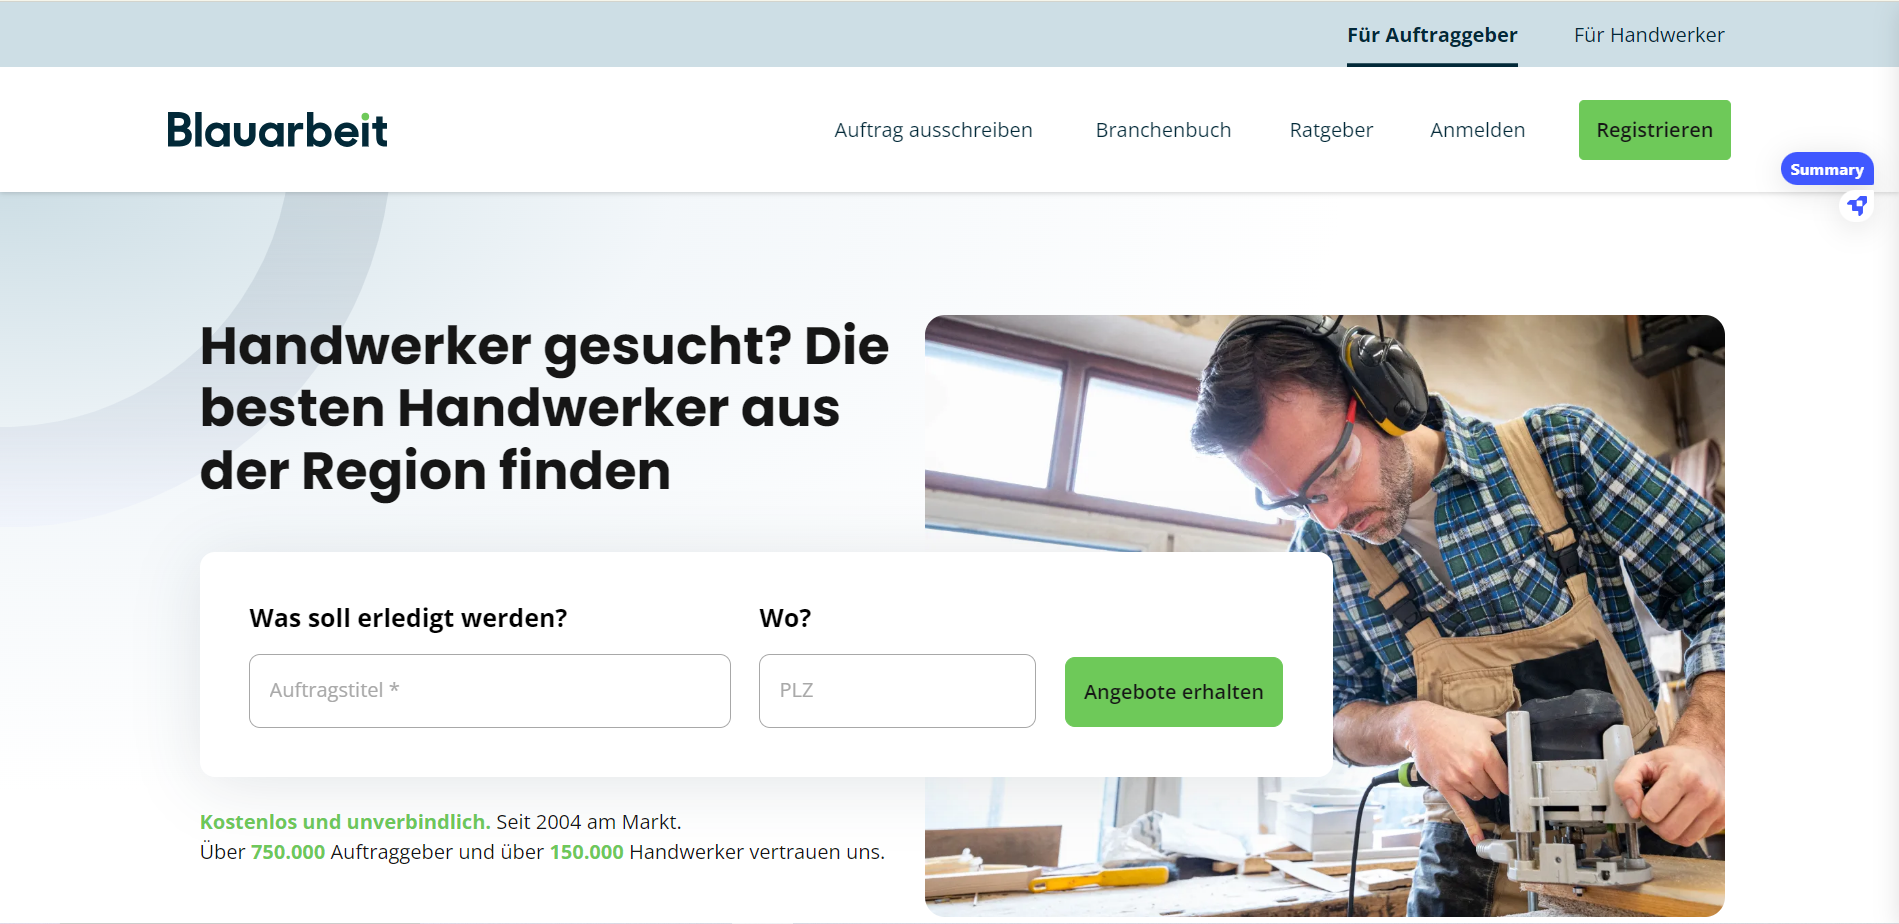
\includegraphics[width=\linewidth]{src/assets/chapters/Blaurabeit.PNG}
    \caption{Blaurabeit Homepage}
    \label{fig:blaurabeit_image}
\end{figure}


\subsection{MyHammer  \cite{MyHammer}}
MyHammer is a German online portal that offers homeowners and businesses the option to find local craftsmen and service providers for a wide variety of construction and repair work. MyHammer offers a set of features such as a huge variety of services provided, transparent bidding, and a mobile-friendly interface. The following figure (Figure \ref{fig:myhammer_image}) shows the MyHammer homepage, highlighting their comprehensive service offerings and user-friendly design.
\begin{figure}[H]
    \centering
    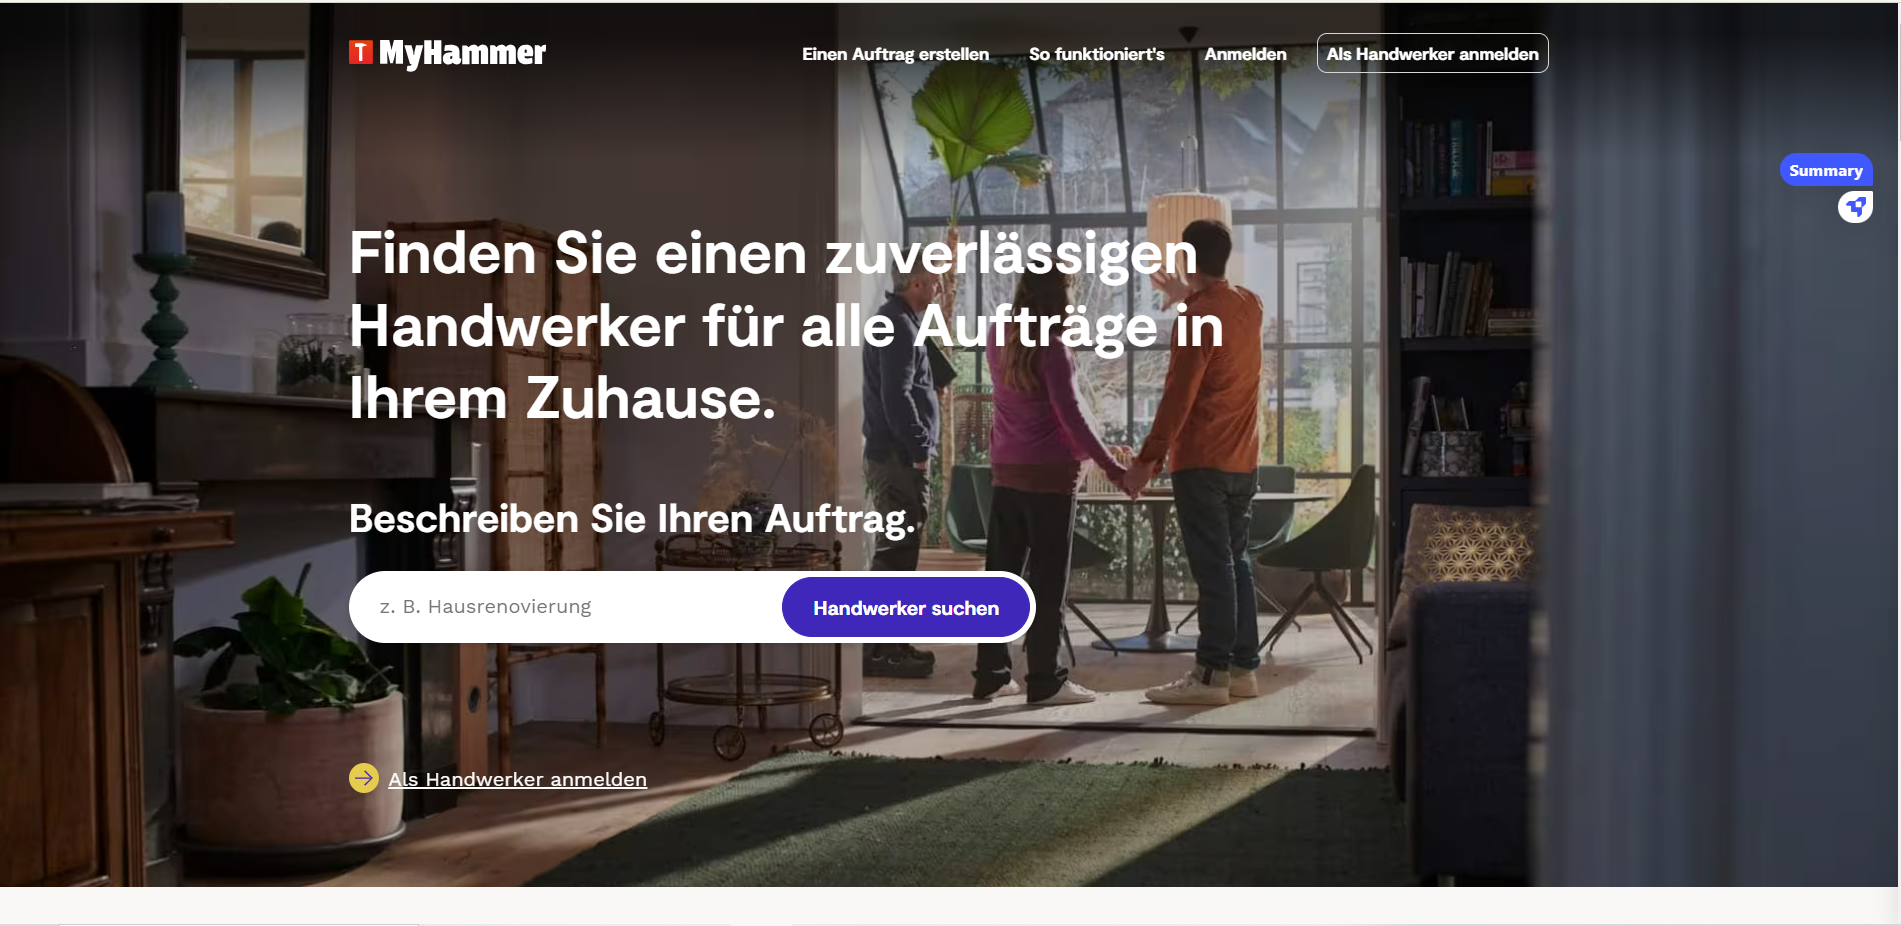
\includegraphics[width=\linewidth]{src/assets/chapters/myHammer.PNG}
    \caption{MyHammer Homepage}
    \label{fig:myhammer_image}
\end{figure}



\subsection{Aermax  \cite{Aermax}}
Aermax is a company that specializes in the provision of services at altitudes. It specializes in works that require preciseness, safety, and expertise. One of the aspects of their work involves the provision of services that ensure buildings last and remain viable for a long time. The following figure (Figure \ref{fig:aermax_image}) shows the Aermax homepage, highlighting their specialized services in industrial alpinism and rope access techniques.

\begin{figure}[H]
    \centering
    
\includegraphics[width=\linewidth]{src/assets/images/aermax.PNG}
    \caption{Aermax Homepage}
    \label{fig:aermax_image}
\end{figure}

\subsection{Competitors Selection}
We are conducting a thorough assessment of project management platforms for industrial climbers to improve user experience and streamline operational processes. We will evaluate their functionalities, strengths, and weaknesses against 7 key criteria tailored to our project's needs and select the platform that best fits our requirements.

\begin{itemize}
    \item \textbf{C1: User Interface:} How the platform is designed regarding the interface and navigation of the platform to create a good experience for both technicians and project managers.

    \item \textbf{C2: Task Management:} How efficient is the platform in managing projects, including task assignment, progress tracking, and deadline setting.

    \item \textbf{C3: Document Management:} How the platform manages project documents, user files, the daily reports and performance’s reports.
    \item \textbf{C4: Communication Tools:} How far the platform supports communication between project managers, worker, and customers including real-time messaging, notifications.

    \item \textbf{C5: Safety Compliance:} How the platform can ensure compliance with safety regulations and standards that pertain to industrial climbing projects, tracking certifications, training records, and safety procedures.
    \item \textbf{C6: Equipment Management:} How the platform manege equipment used for industrial climbing projects.
    \item \textbf{C7: Project Planning and Scheduling:} How efficient the platform is in project planning and scheduling features, and timeline management.
\end{itemize}

\begin{longtable}{|p{2cm}|p{3.5cm}|p{3.5cm}|p{3.5cm}|}
    % Table header information for the first part
    \caption{Comparison of Project Management Platforms for Industrial Climbers} \\
    \hline
    \textbf{Criteria} & \textbf{MyHammer} & \textbf{Blauarbeit} & \textbf{Aermax}  \\
    \hline
    \endfirsthead
    
    % Table continuation header information
    \hline
    \textbf{Criteria} & \textbf{MyHammer} & \textbf{Blauarbeit} & \textbf{Aermax}  \\
    \hline
    \endhead
    
    % Footer at the end of each page (if needed)
    \hline
     
    
    % Footer at the end of the table (if needed)
    \hline
    \endlastfoot
    
    % Table content for Part 1
    C1: User Interface &  User-friendly interface for homeowners and service providers to connect for  projects.& Straightforward interface for customers and service providers to post and bid on household service tasks. & Easy-to-use design for admins, workers, and customers. The UI lacks a lot of refinments. \\ 
    \hline
    C2: Task Management & Lack of a dedicated task management features for organizing and tracking project progress. &  Lack of a dedicated task management features.Blauarbeit  does not offer tools specifically for task management within projects. & Essential task management features for project organizing and tracking progress is what Aermax provides. \\
    \hline
    C3: Document Management & Lack of a dedicated document management features. & Lack of a dedicated document management features. & Aermax provide a whole separe service to document management
    \\
    \hline
    
    % Table content for Part 2, continues in the same longtable environment
    C4: Communication Tools & A basic communication tool for homeowners and service providers to discuss project details and negotiate terms. & A standard communication tool for customers and service providers to negotiate job requirements and arrangements. & A standard chat channel for admins and workers, to discuss project progress and details. \\
    \hline
    C5: Safety Compliance & No specific safety compliance features for home improvement projects. & No dedicated safety compliance features for household services. & Lack of safety compliance features for construction and climbing services. \\
    \hline
    C6: Equipment Management & A fully integrated equipment management tool, to automate tracking and  management of equipment assets that can be used to complete projects efficiently. & An automated equipment management feature, providing scalable solutions for tracking and managing equipment assets across projects. & A simple and standard equipment management feature which isn’t maintainable and extensible.\\
    \hline
    C7: Project Planning and Scheduling & Lack of specific project planning or scheduling tools. & Lack of specific project planning or scheduling tools. & An efficient tool for managing and planning projects. \\
    \hline
\end{longtable}

% ----------------------- Assessment of the case ----------------------- %
\section{Assessment of the case}
This chapter shall evaluate the current state of the project, its strengths and weaknesses, propose solutions for its issues, and outline its implementation steps. The systematic approach is aimed at enhancing the performance of the project and user satisfaction.

\subsection{Describing the work procedure}
The work on any project, first of all, needs to be preceded by the profound study of the existing ones, undermining the strengths and weaknesses of the current system, and business decisions which should be taken into account during the conception and realization.
\subsection{Criticizing the current state}
After studying the existing, we can determine its limitations:
\subsubsection{Functional Issues}
\begin{itemize}
    \item Functionalities are not working as expected.
    \item New features are yet to be developed.
    \item Parts of the application need complete overhauling to meet the client's requirements.
\end{itemize}


\subsubsection{Technical Issues}
\begin{itemize}
    \item Since cron jobs are running for the whole day, bugs are hard to respond to fast enough because we can only deploy once at the end of the day.
    \item Many bugs remain unfixed.
    \item The code needs refactoring due to some bad practices that make the app take more time to execute.
\end{itemize}

\subsection{Proposed solution}
With the problems identified, we make the following proposals for the way forward.

\begin{itemize}
    \item First, existing features will be enhanced to ensure that they work as they should. This will entail a keen review and subsequent test of the features to identify and fix any bugs.
    \item In addition, new features will be developed based on priority to ensure that the application meets all of the client's requirements.
    \item There will also be thorough refactoring of the codebase to remove bad practices and optimize performance.
    \item The UI/UX is also recommended to be enhanced for a better user experience. The proposed solutions should be aimed at greatly enhancing the general performance of the application, reliability, and user satisfaction.
    \item Build a new feature: Reward System to make Aermax's users more engaged and motivated.
\end{itemize}

The following figure (Figure \ref{fig:Reward_System_explain_image}) provides an overall view of the proposed Reward System for Aermax. This system is designed to transform the user experience by making tasks more engaging and rewarding.

\begin{figure}[H]
    \centering
    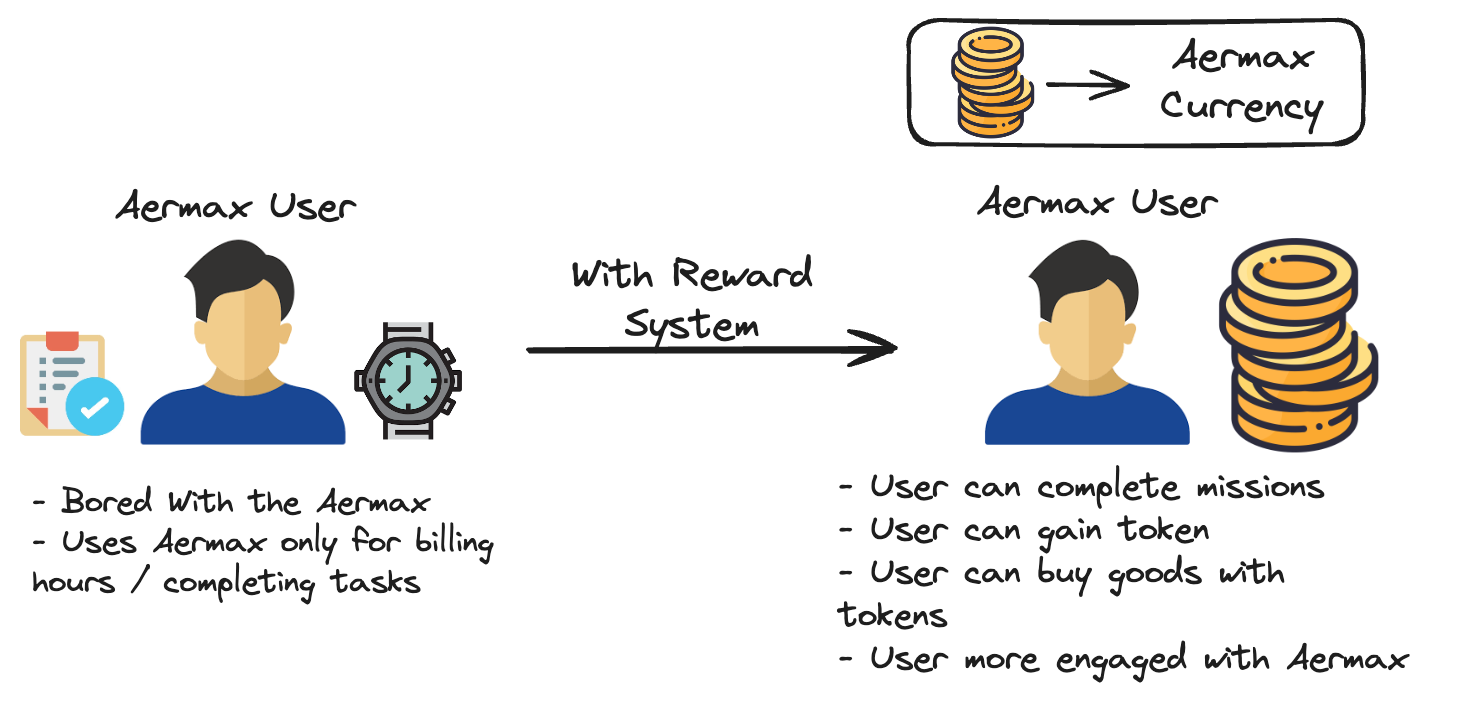
\includegraphics[width=1\textwidth]{src/assets/diagrams/rewardexplain.png}
    \caption{Reward System Overall View}
    \label{fig:Reward_System_explain_image}
\end{figure}

The next figure (Figure \ref{fig:Reward_System_detailed_explain_image}) illustrates the detailed scenario of how the Reward System works within the Aermax platform. It highlights the process of creating missions, gaining tokens and XP, and using them in the Aermax store.

\begin{figure}[H]
    \centering
    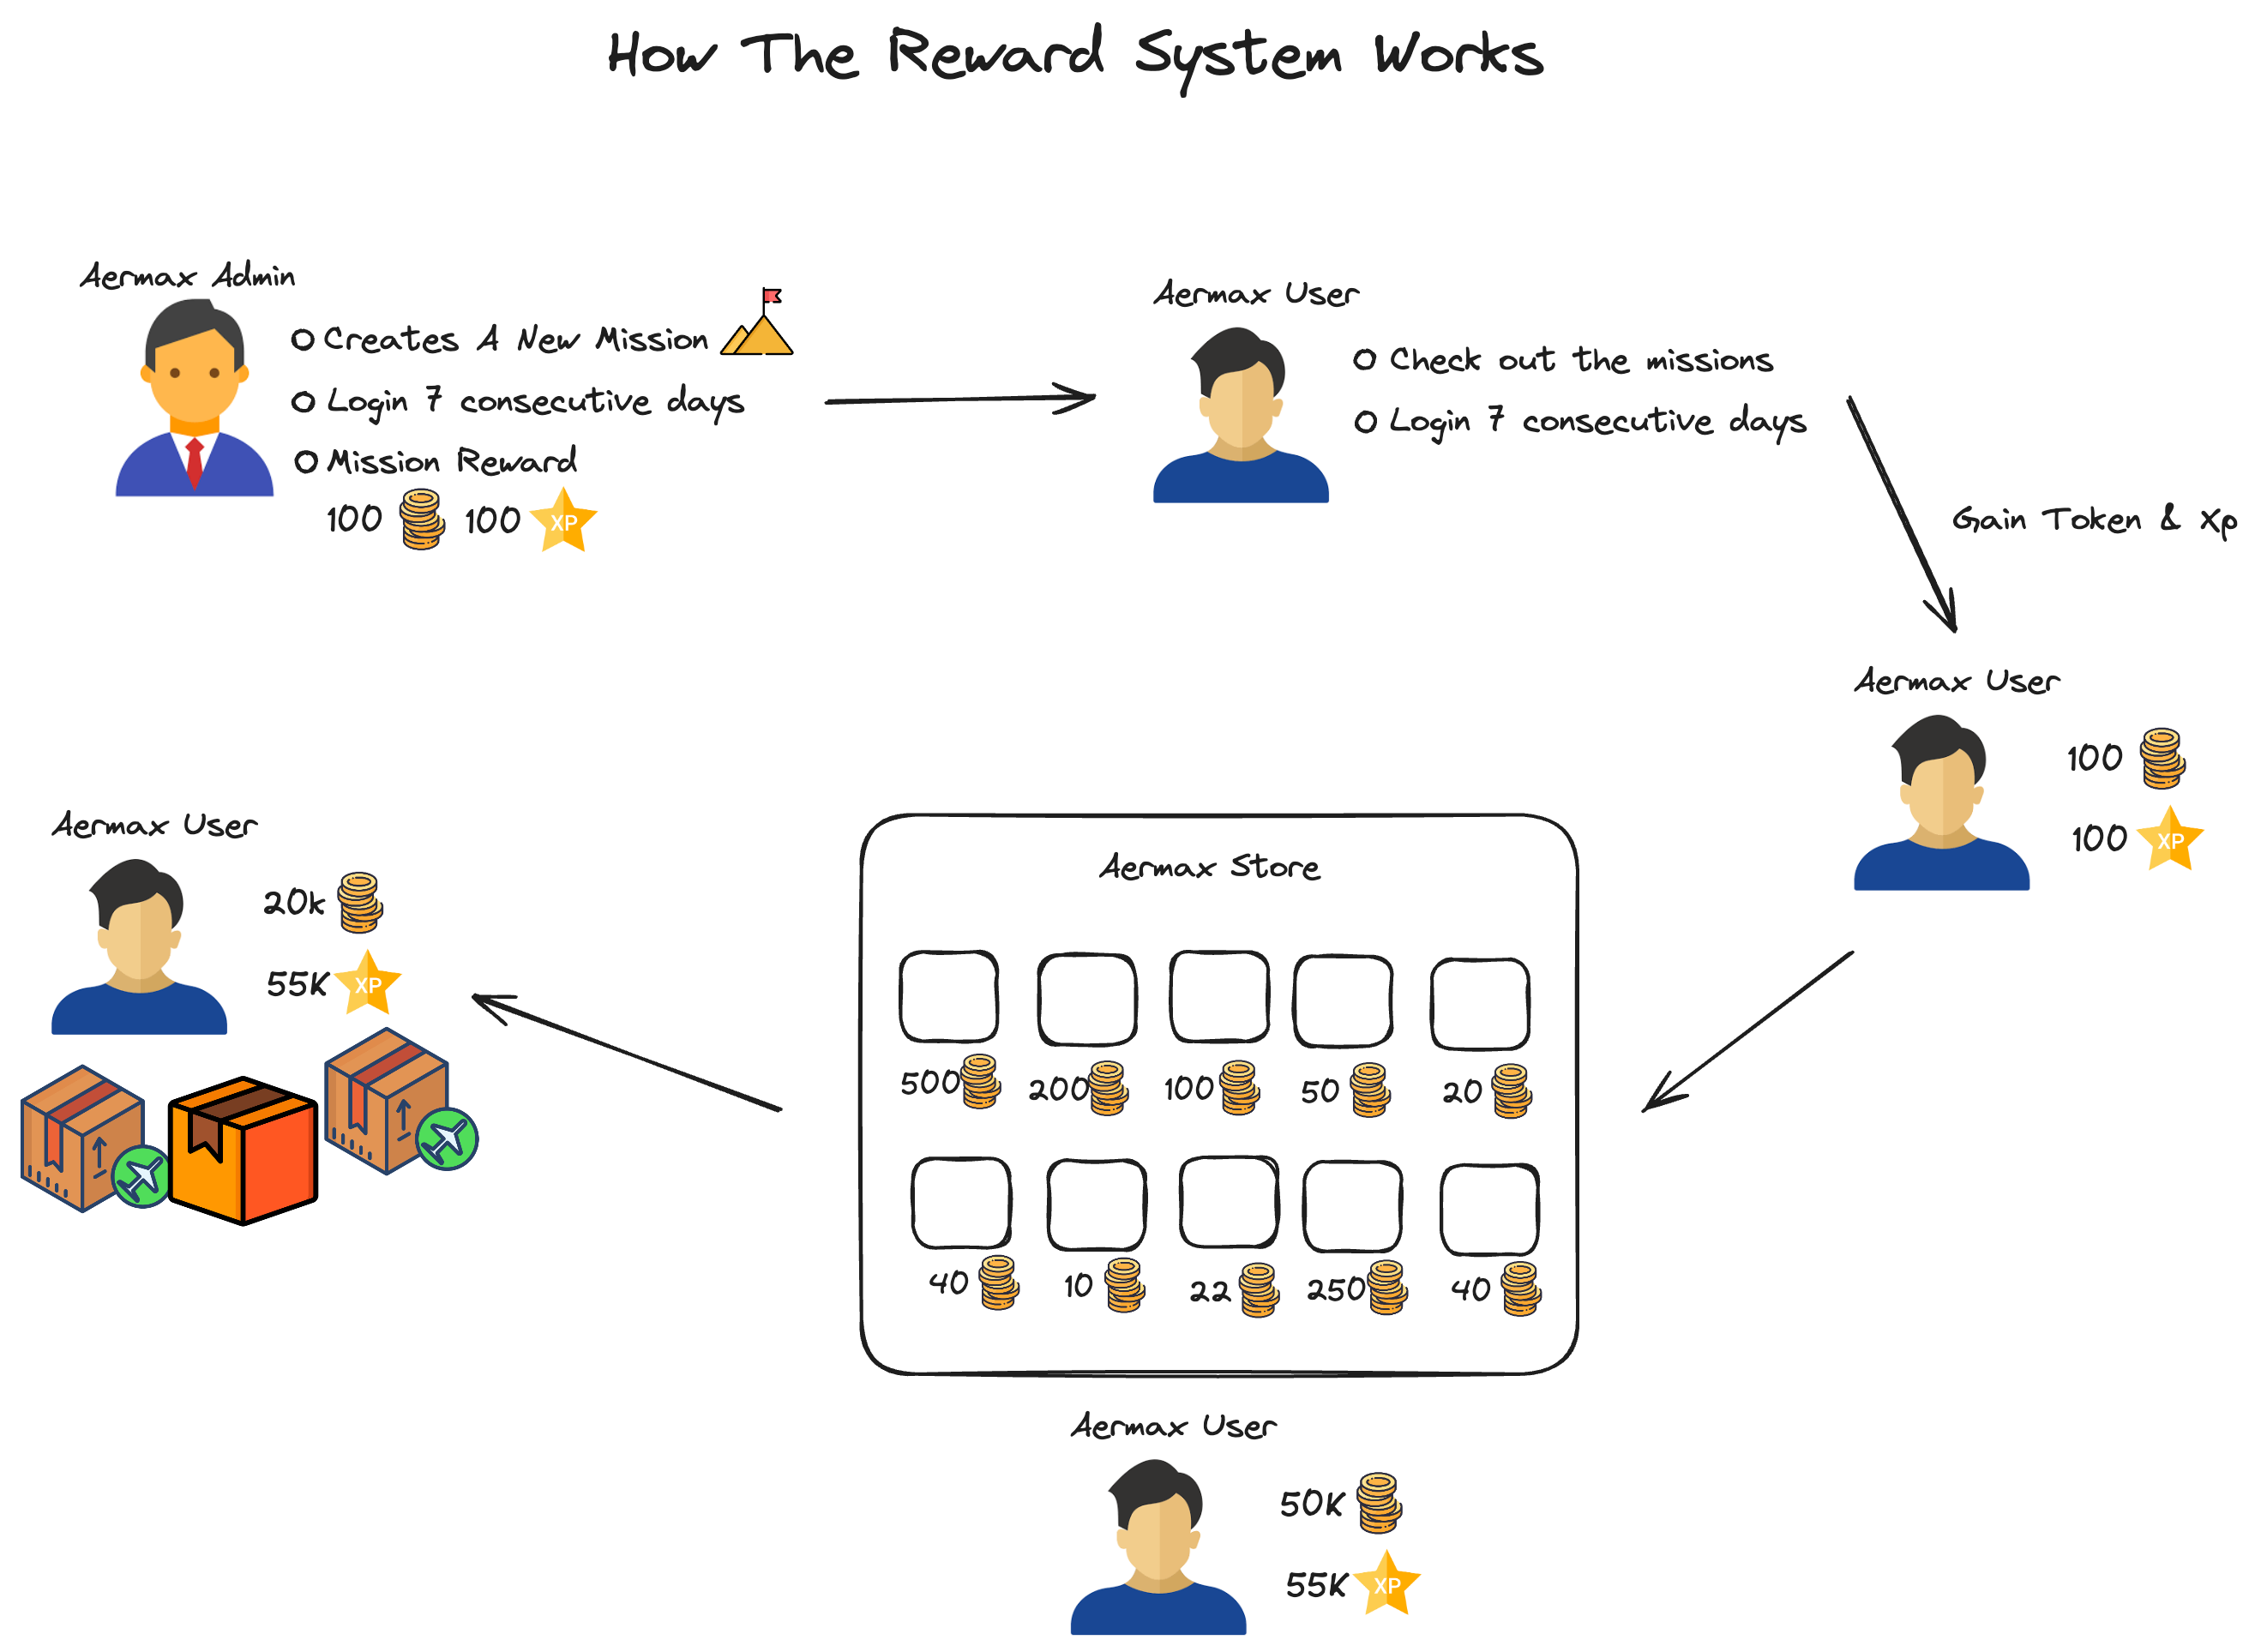
\includegraphics[width=1\textwidth]{src/assets/diagrams/rewardexplain2.png}
    \caption{Reward System Detailed Scenario}
    \label{fig:Reward_System_detailed_explain_image}
\end{figure}
   
% ----------------------- Development Methodology ----------------------- %
\section{Development Methodology}
The development methodology adopted for this project is aimed at ensuring flexibility, efficiency, and responsiveness to changes. This approach is particularly suitable for dynamic environments where requirements can evolve over time, and continuous improvement is crucial.

\subsection{Agile methodology}
Agile is a structured and iterative approach to project management and product development.
It recognizes the volatility of product development, and provides a methodology for self-organizing teams to respond to change without going off the rails.

\subsection{Scrum methodology}
The Scrum team commits to the completion of an increment of work, which is potentially shippable, through set periods of time called sprints. They strive to build a learning loop in order to quickly collect and integrate customer feedback. Scrum teams embrace specific roles, create special artifacts, and hold regular ceremonies to keep things moving. The following figure (Figure \ref{fig:Scrum_Framework_image}) illustrates the Scrum framework, showcasing the key components and processes involved.

\begin{figure}[H]
    \centering
    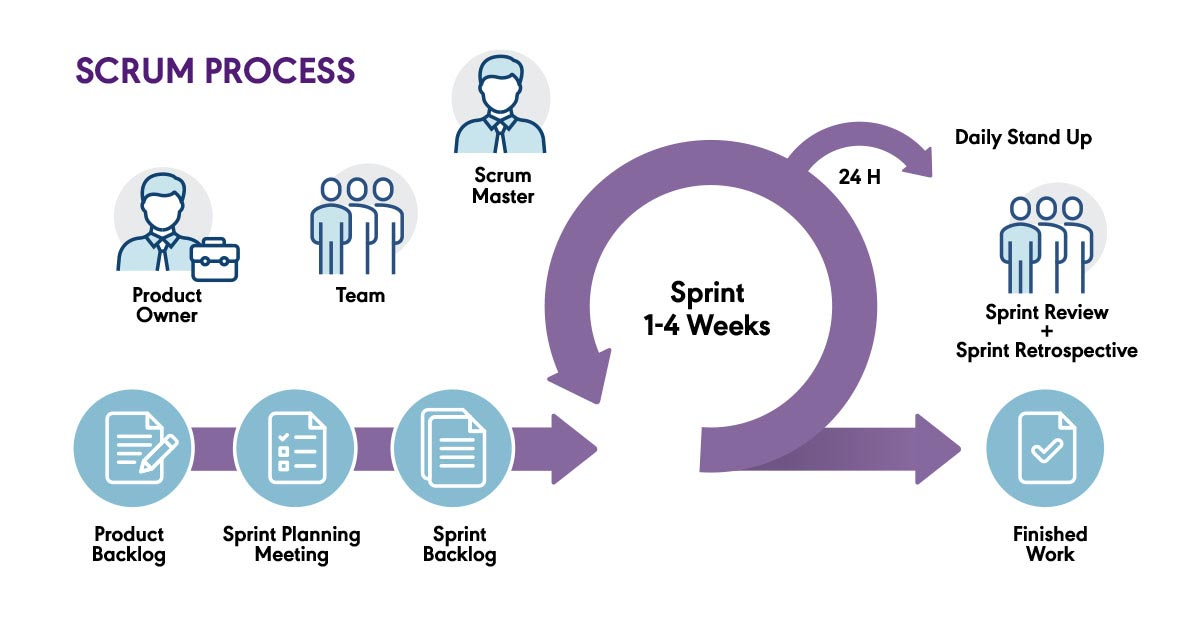
\includegraphics[width=1\textwidth]{src/assets/chapters/blog-scrum-process-opt.jpg}
    \caption{The Scrum Framework}
    \label{fig:Scrum_Framework_image}
\end{figure}


\subsection{Kanban methodology}
Kanban is all about visualizing your work, limiting work in progress, and maximizing efficiency (or flow).
Kanban teams focus on reducing the time a project takes from start by using a Kanban board to continuously improve their flow of work.
To explain more in details, Kanban is based on a continuous workflow structure that keeps teams nimble and ready to adapt to changing priorities.
Work items —represented by cards— are organized on the board where they flow from one stage of the workflow or column to the next.
Common workflow stages are To Do, In Progress, In Review, and Done.

\subsection{Scrumban methodology}
ScrumBan is a hybrid Agile methodology that combines elements of Scrum and Kanban. Here are some important points about Scrumban:

\begin{itemize}
    \item Hybrid Methodology: ScrumBan merges the flexibility of Kanban with the structure of Scrum to optimize workflow.
    \item Continuous Improvement: Similar to Kanban, Scrumban focuses on continuous improvement with the visualization of workflow and by limiting Work in Progress (WIP).
    \item Iterative Approach: Scrumban retains the iterative approach of Scrum—allowing periodic review and adaptation of processes.
    \item Adaptive Planning: A team can plan in a way that it can change the priorities and resources, if so required, as per the changing requirements while using Scrumban.
    \item Lean Principles: Scrumban adopts the principles of Lean—like waste elimination and maximization of value delivery—to streamline processes.
\end{itemize}
The following figure (Figure \ref{fig:Scrumban_image}) shows the Scrumban board, illustrating how this hybrid methodology combines the best practices of Scrum and Kanban to optimize workflow and enhance productivity
\begin{figure}[H]
    \centering
    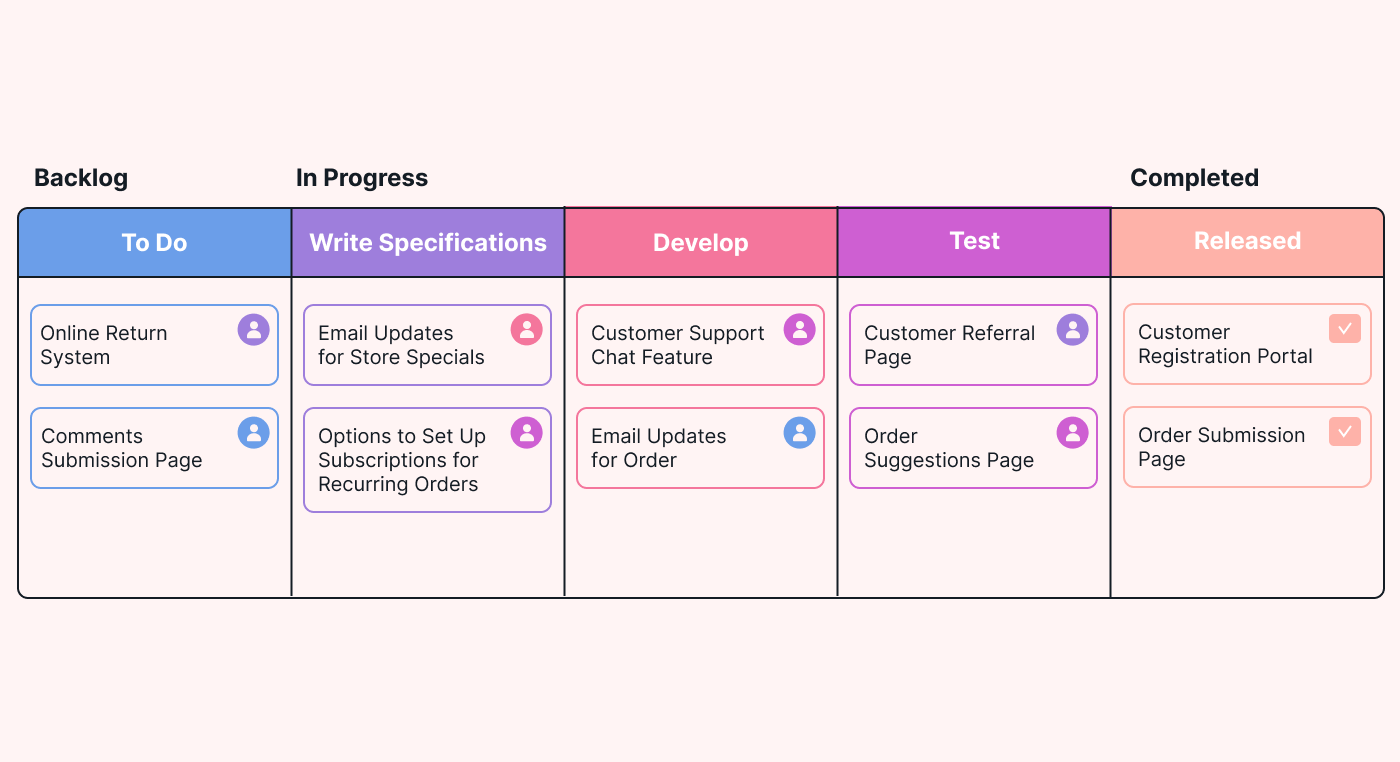
\includegraphics[width=0.7\textwidth]{src/assets/chapters/Scrumban.png}
    \caption{The Scrumban board}
    \label{fig:Scrumban_image}
\end{figure}

\subsection{Choice of development methodology}
Scrumban has been chosen as the preferred development methodology for the following reasons:
\begin{itemize}
    \item \textbf{Flexibility:} ScrumBan is a very flexible approach that brings some structure to Scrum while maintaining a high level of adaptability, similar to Kanban, which includes fast responses to changing priorities while maintaining a framing order for work.
    \item \textbf{Continuous Improvement:} Scrumban encourages continuous improvement, and teams can evolve their process over time.
    \item \textbf{Reduced Waste:} Scrumban introduces the principle of just-in-time delivery of user stories and WIP limits to ensure minimization of wastes.
    \item \textbf{Improved Visibility:} Visual boards improve the visibility of work, enabling transparency and encouraging collaboration.
    \item \textbf{Optimized Flow:} Scrumban is a way of optimizing flow by balancing Kanban flexibility with structured Scrum, enabling teams to build value consistently and predictably.
\end{itemize}
The following figure (Figure \ref{fig:armax-board}) shows the Aermax Board, illustrating how Scrumban is implemented to manage tasks and workflow effectively within the team.
\begin{figure}[H]
    \centering
    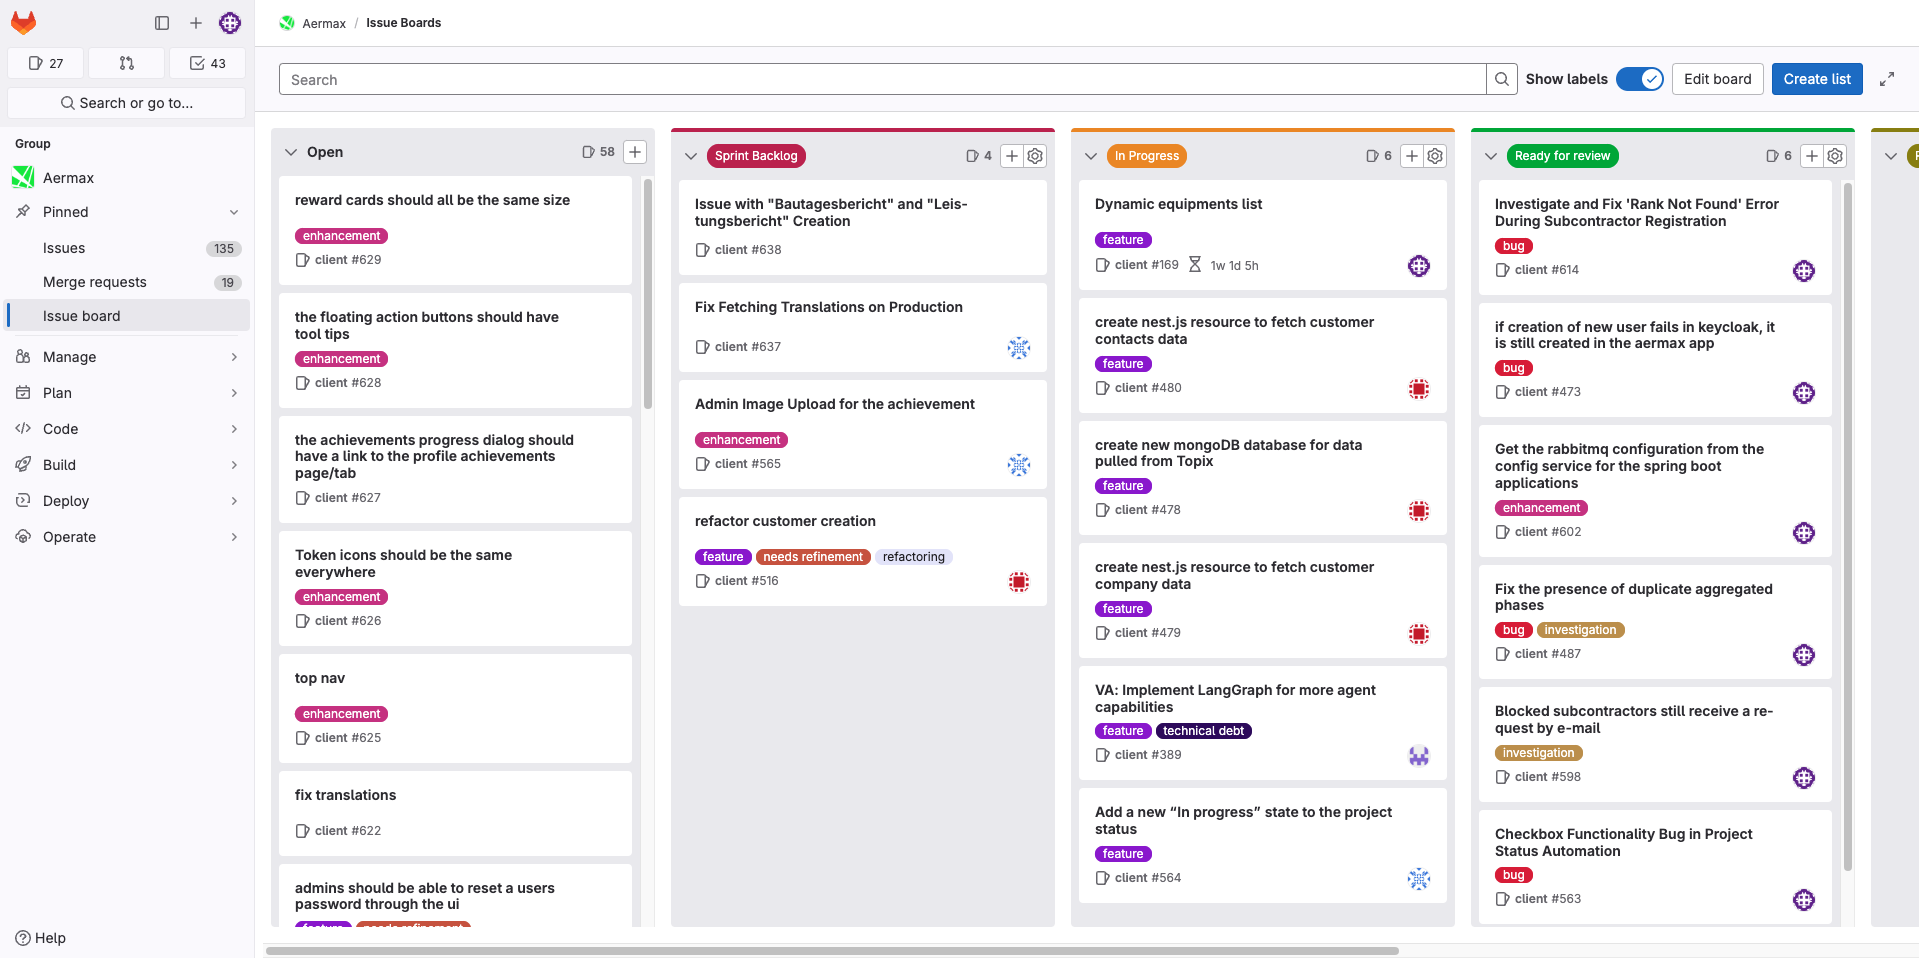
\includegraphics[width=1\textwidth]{src/assets/chapters/aermax-board.png}
    \caption{Aermax Board}
    \label{fig:armax-board}
\end{figure}
\subsection{Unified Modeling Language}
The Unified Modeling Language (UML) is a general-purpose, developmental, modeling language in the field of software engineering that is intended to provide a standard way to visualize the design of a system. In our case, we used UML to design the top level view of the systems therefore we only used the Use Case and Sequence diagrams.

\setcounter{secnumdepth}{0} % Set the section counter to 0 so next section is not counted in toc
% ----------------------- Conclusion ----------------------- %
\section{Conclusion}
This chapter introduces the host organization, assesses identified problems and associated challenges, evaluates the competitive landscape, and the adoption of an agile methodology by the team. It also speaks to the next chapter, which is going to deal with the setting of objectives and laying out the roadmap for the remaining sprints under Sprint 0.

\chapter{ Sprint 0 : Project Initialization}
\phantomsection


\setcounter{secnumdepth}{0} % Set the section counter to 0 so next section is not counted in toc

% ----------------------- Introduction ----------------------- %

\section{Introduction}
In this chapter, we delve into the comprehensive specifications and requirements that form the foundation of the Aermax project. We will explore the essential features of the product, providing a clear understanding of its capabilities and objectives. Additionally, we will identify and describe the key stakeholders involved in the project, highlighting their roles and how they interact with the system. This foundational analysis sets the stage for the subsequent development sprints and ensures all participants have a shared vision and understanding of the project goals.
\setcounter{secnumdepth}{3}
\section{Overview of the Project}
The Aermax project is an extensive endeavor focused on creating a robust and scalable platform by integrating both existing and newly developed microservices.  \\
This section identifies the key stakeholders involved, highlighting their roles and responsibilities. The Aermax project involves various stakeholders who play crucial roles in its operation and success. The key stakeholders and their roles are summarized in the table below. The grey-highlighted rows represent external stakeholders, while the non-highlighted rows represent internal stakeholders.
\begin{table}[h!]
    \centering
    \renewcommand{\arraystretch}{1.5} % Padding
    \caption{Stakeholders and their Roles}
    \label{tab:stakeholders_roles}
    \begin{tabularx}{\textwidth} {
            | >{\hsize=0.4\hsize\linewidth=\hsize\raggedright\arraybackslash}X
            | >{\hsize=1.6\hsize\linewidth=\hsize\raggedright\arraybackslash}X |}
        \hline
         \textbf{Role} & \textbf{Description} \\
        \hline
        Admin & Responsible for managing the overall system, including user management, system configuration, and monitoring. \\
        \hline
        \rowcolor{gray!20} Subcontractor & Industrial climbers who perform specific tasks or services outside the direct supervision of the project manager. \\
        \hline
        Employee & Internal staff members who work on various aspects of the project under the guidance of the project manager. \\
        \hline
        Project Manager & Oversees the project's progress, manages timelines, and ensures that all aspects of the project are aligned with strategic goals. \\
        \hline
        \rowcolor{gray!20} Leader & Provides vision and direction for the project, making high-level decisions and ensuring that the project aligns with organizational objectives. \\
        \hline
    \end{tabularx}
\end{table}
\FloatBarrier
\section{Functional Requirements}
Functional requirements define the specific behaviors and functionalities that the system must possess to meet user needs. This section focuses on the key functional requirements for our project, particularly the reward system and other essential functionalities.

\subsection{Feature Enhancement}

This section details the latest upgrades and additions made to our system. These enhancements aim to improve functionality, usability, and overall user satisfaction. Key features introduced are:

\begin{itemize}
    \item \textbf{Dynamic Equipment List:} Implement a dynamic list of equipment that updates in real-time based on user selections and other criteria.
    \item \textbf{Bug Fixes:} Identify and fix several bugs in the existing functionalities to ensure a smooth user experience.
    \item \textbf{Enhanced Packet View:} Enhance the packet view by adding new functionalities and improving existing features.
    \item \textbf{Project Status Overhaul:} Overhaul the project status feature, including data migration to support the new structure.
    \item \textbf{Role System Overhaul:} Overhaul the role system to provide more granular control and better user management.
\end{itemize}

\subsection{Reward System}
As mentioned in Chapter 1, Section I.5.3, we provided an overview of the reward system designed to enhance user engagement and motivation. In this chapter, we will delve deeper into the specifics of the reward system, which is fundamentally based on Experience Points (XP), Tokens, and Levels/Ranks.

The image below illustrates the core components of our reward system. On the left side, the climber symbolizes user progression through the ranks, carrying a sack of tokens that represents the accumulated rewards. On the right, the various rank logos are displayed, indicating the different levels users can achieve as they gain XP and move up in the hierarchy.
\begin{figure}[H]
    \centering
    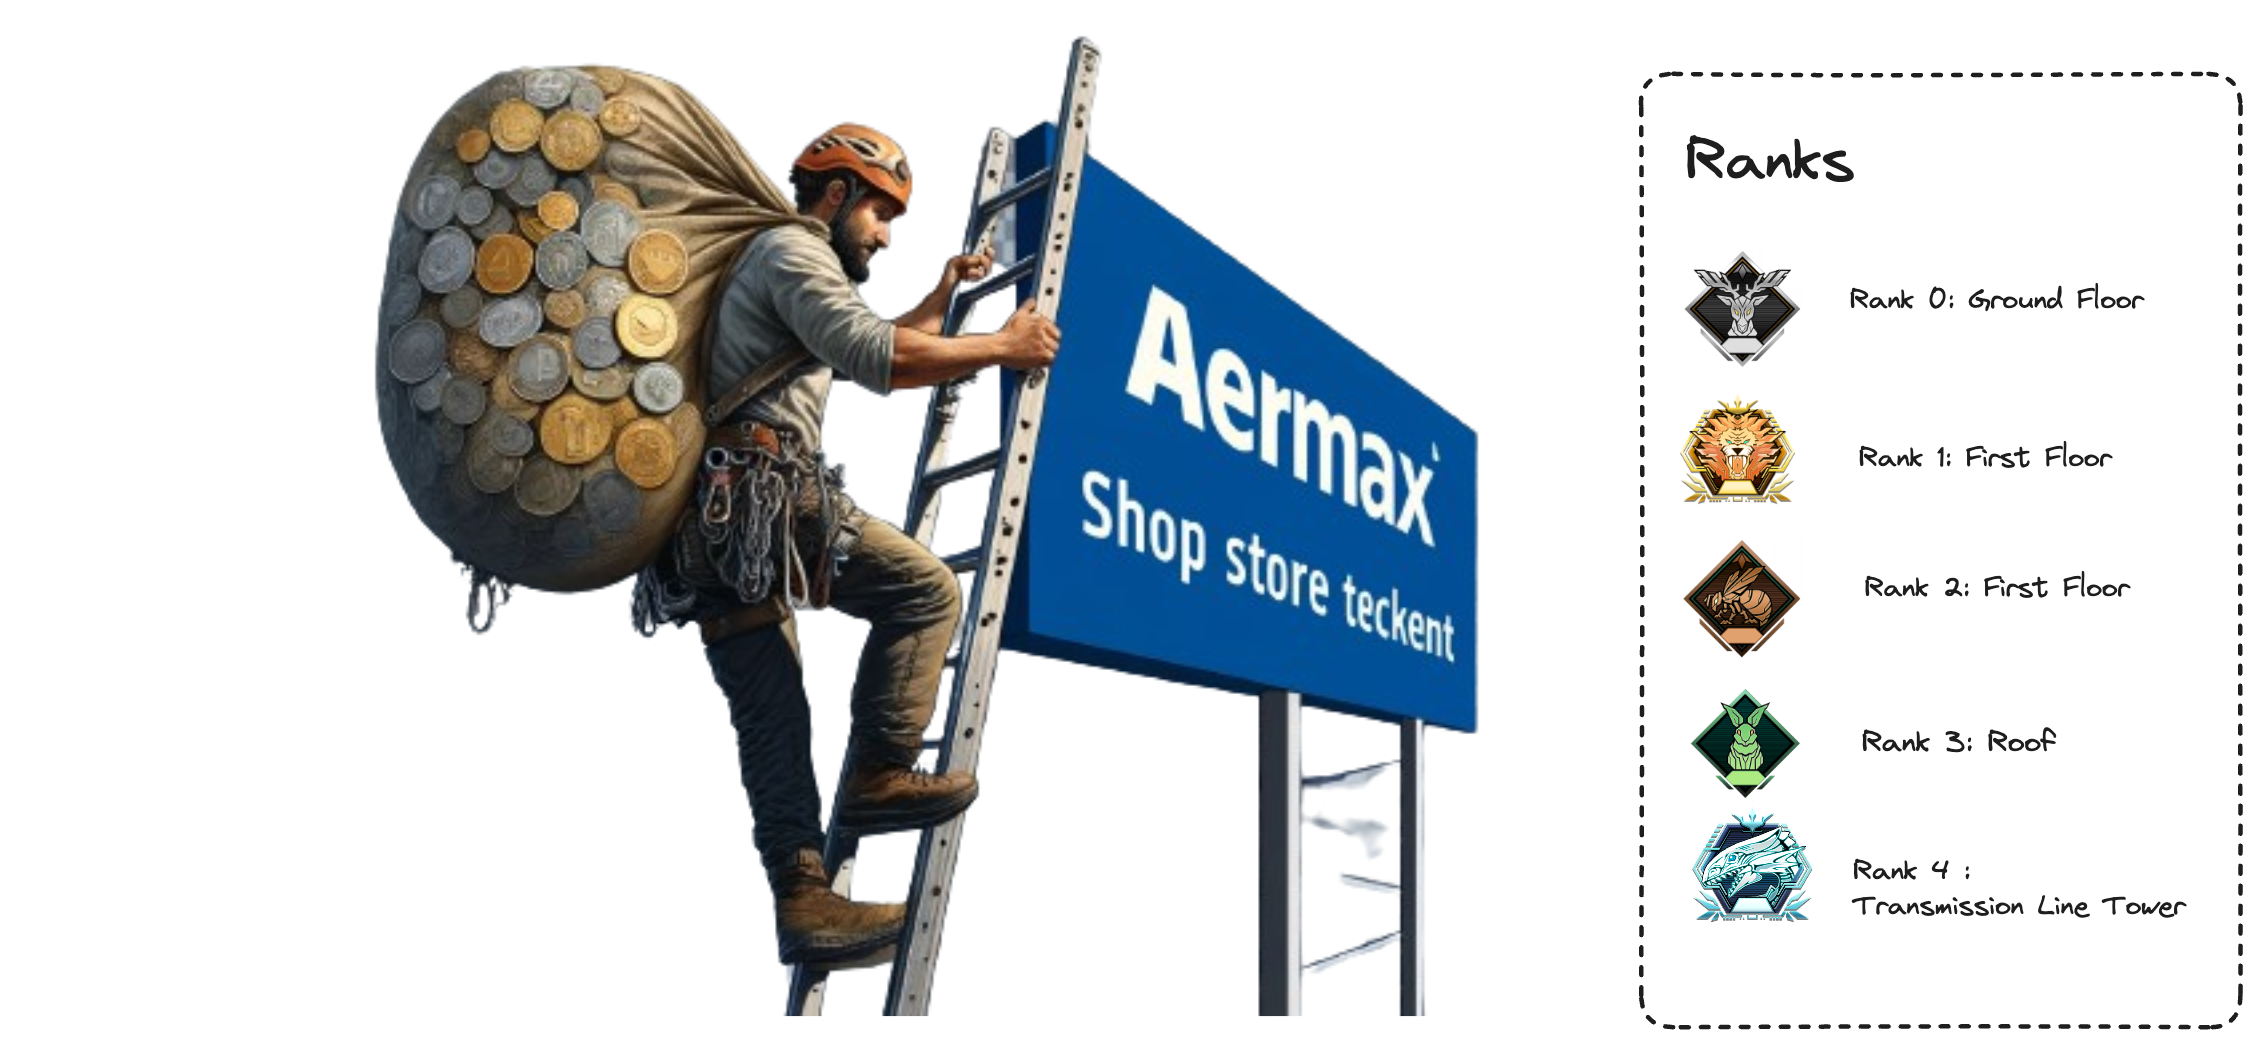
\includegraphics[width=1\textwidth]{src/assets/images/AermaxClimberPng.png}
    \caption{User Progression}
    \label{fig:user_progression}
\end{figure}

\textbf{Tokens:} Tokens are a form of currency earned through specific activities and can be redeemed for rewards.

\textbf{XP (Experience Points):} XP is earned by users as they complete tasks and participate in activities, reflecting their progress and engagement.

To support this system, comprehensive algorithms must be developed to calculate rewards and progress behind the scenes. To ensure the effectiveness and accuracy of these algorithms, a simulator was used to visualize and clarify the reward system before actual development began. Each rank in the system has multiple levels, and progressing through these levels requires accumulating a specific amount of XP (Experience Points). This approach leverages gamification principles to keep users engaged and motivated by offering continuous challenges and rewards (see Figure \ref{fig:reward_system_simulator}).

\begin{figure}[H]
    \centering
    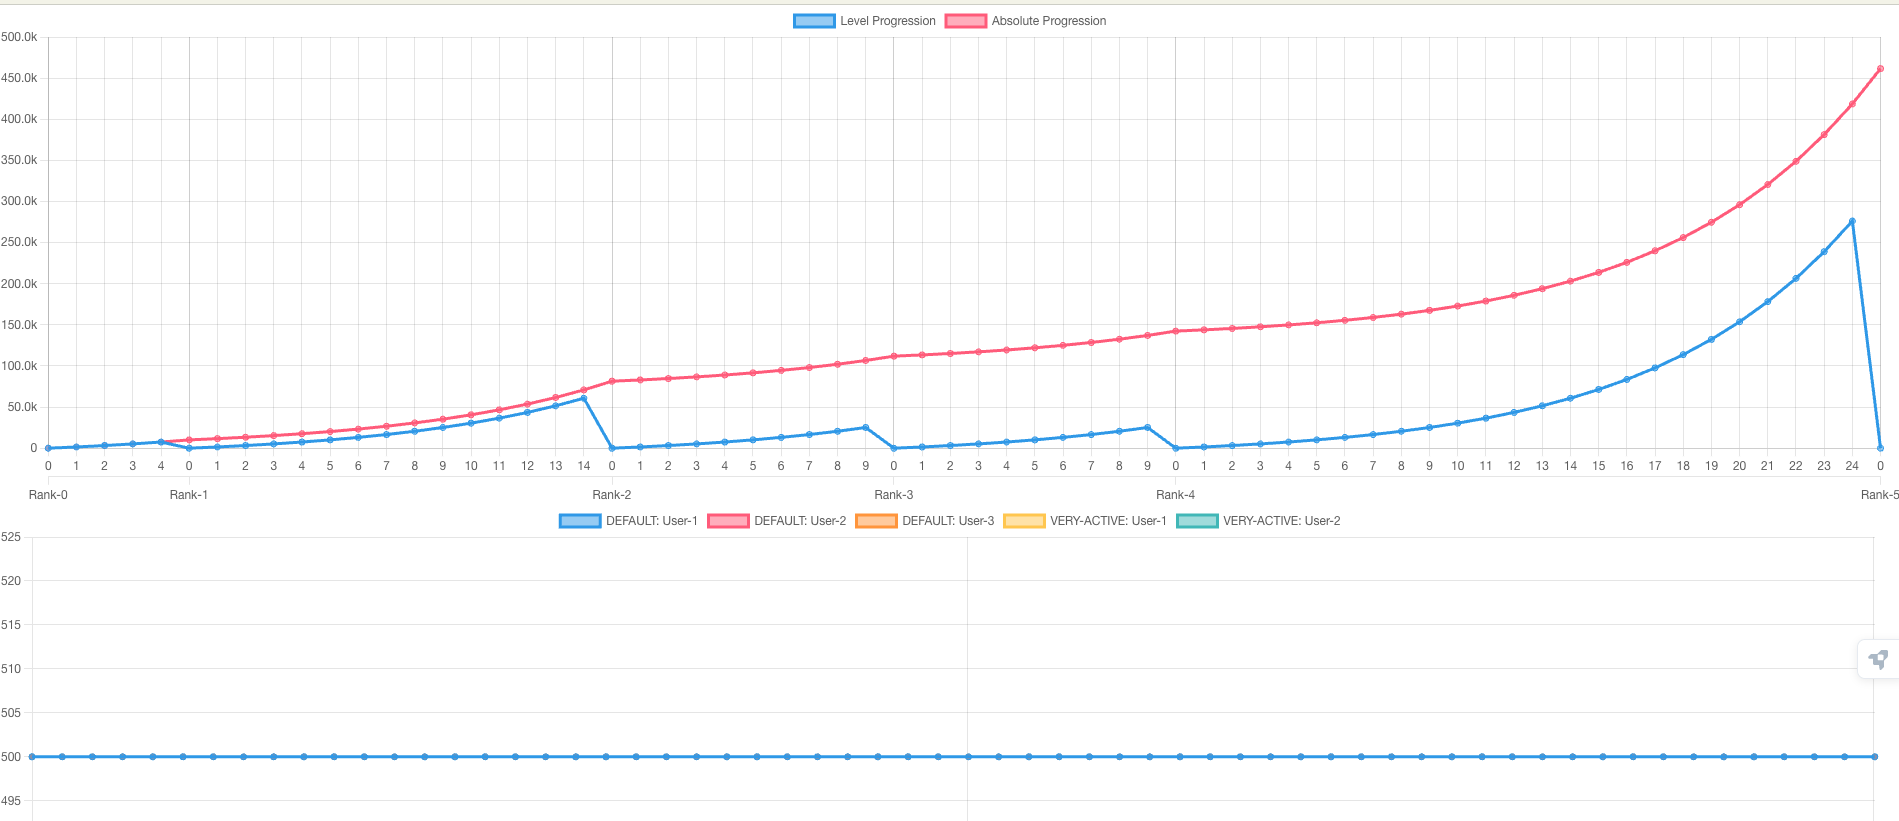
\includegraphics[width=1\textwidth]{src/assets/images/simulator.png}
    \caption{Reward System simulator}
    \label{fig:reward_system_simulator}
\end{figure}

This simulator helps in understanding how users will interact with the reward system, ensuring that the designed algorithms for XP and level progression are effective and engaging.
 

\section{Technical Requirements}
Technical requirements specify the underlying technical aspects and constraints necessary for the system to function correctly. This section outlines the technical requirements that support the functional requirements.

\subsection{Data Management}
Proper data management is essential for the application's integrity and reliability. The system must provide the following technical functionalities:

\begin{itemize}
    \item \textbf{Database Integration:} The application should interact with multiple databases, such as 'reward-service-db' and 'config-service-db,' to store and retrieve data efficiently.
    \item \textbf{Data Synchronization:} Ensure data consistency and synchronization across different services and databases. Handle operations that span multiple microservices.
    \item \textbf{Data Security:} Implement robust security measures to protect sensitive user data, including encryption, access control, and regular security audits.
\end{itemize}

\subsection{System Integration}
Seamless integration with various external and internal systems is crucial for the application's operation. Key technical integration functionalities include:

\begin{itemize}
    \item \textbf{RabbitMQ Configuration:} Retrieve and manage RabbitMQ configurations from the config service for different microservices. Ensure reliable message queuing and processing.
    \item \textbf{Health Checks:} Implement health checks for various microservices to monitor their status and ensure they are operating correctly.
    \item \textbf{Deployment Pipeline:} Set up a deployment pipeline for staging and production environments, including automated testing, deployment, and monitoring of the reward system.
\end{itemize}

% --------------- Non-functional Requirements --------------- %

\section{Non-functional Requirements}
Non-functional requirements describe any specification that does not add direct business value but is nonetheless crucial for the good operation of developed software.
For Aermax, what we should focus on is:
\begin{itemize}
	\item \textbf{Reliability and Availability:} The software should be available 24 hours a day and 7 days a week.
	\item \textbf{Security:} Clients should be able to safely log in to the dashboard with a strong authentication system.
	\item \textbf{Scalability:} This is the main reason we're using new microservices.
	\item \textbf{Documentation:} We should always document each and every step we make extensively so that new developers can onboard on the project in a fast and efficient way, which further emphasizes reliability.
\end{itemize}


\section{Aermax Architecture}

The following table provides a comprehensive overview of all the application's microservices, detailing their functionalities and scalability.

\textbf{Table 9: All the Application’s Microservices}
\begin{longtable}{|p{3cm}|p{7cm}|p{2cm}|}
    \hline
    \textbf{Name} & \textbf{Description} & \textbf{Scalable} \\
    \hline
    \endhead
    ai-service & Manages AI operations, including data processing and ML algorithms. & Yes \\
    \hline
    user-service & Handles user data, security, and support functions. & Yes \\
    \hline
    operations-service & Coordinates project management and operational workflows. & Yes \\
    \hline
    storage-service & Oversees data storage and database management. & Yes \\
    \hline
    client & Provides the user interface and input processing. & Yes \\
    \hline
    reward-service & Manages the reward system, including points accumulation, redemption, and catalog maintenance. & Yes \\
    \hline
    config-service & Stores and retrieves configuration settings for various services. & Yes \\
    \hline
\end{longtable}

\begin{itemize}
    \item \textbf{Existing Microservices}:
    \begin{itemize}
        \item \textbf{Operation Service}: Manages operations and interacts with the Operation Database .
        \item \textbf{User Service}: Handles user-related functionalities and interfaces with the User Database.
        \item \textbf{Keycloak Service}: Provides authentication and authorization services, connected to the Keycloak Database.
    \end{itemize}
    Our contributions to these existing microservices include adding new features, enhancements, and bug fixes.
    \item \textbf{New Microservices}:
    \begin{itemize}
        \item \textbf{Reward Service}: Manages reward-related processes and connects to the Reward Database. This service was developed from scratch.
        \item \textbf{Config Service}: A centralized microservice that interacts with all other microservices to provide configuration settings for the reward system. This service was also developed from scratch.
    \end{itemize}
\end{itemize}

This architecture supports modularity, scalability, and efficient management, ensuring consistent configurations and secure authentication through Keycloak. The diagram below (Figure \ref{fig:aermax-architecture}) illustrates the integration of existing and newly developed microservices within a unified virtual network environment.
\begin{figure}[H]
    \centering
    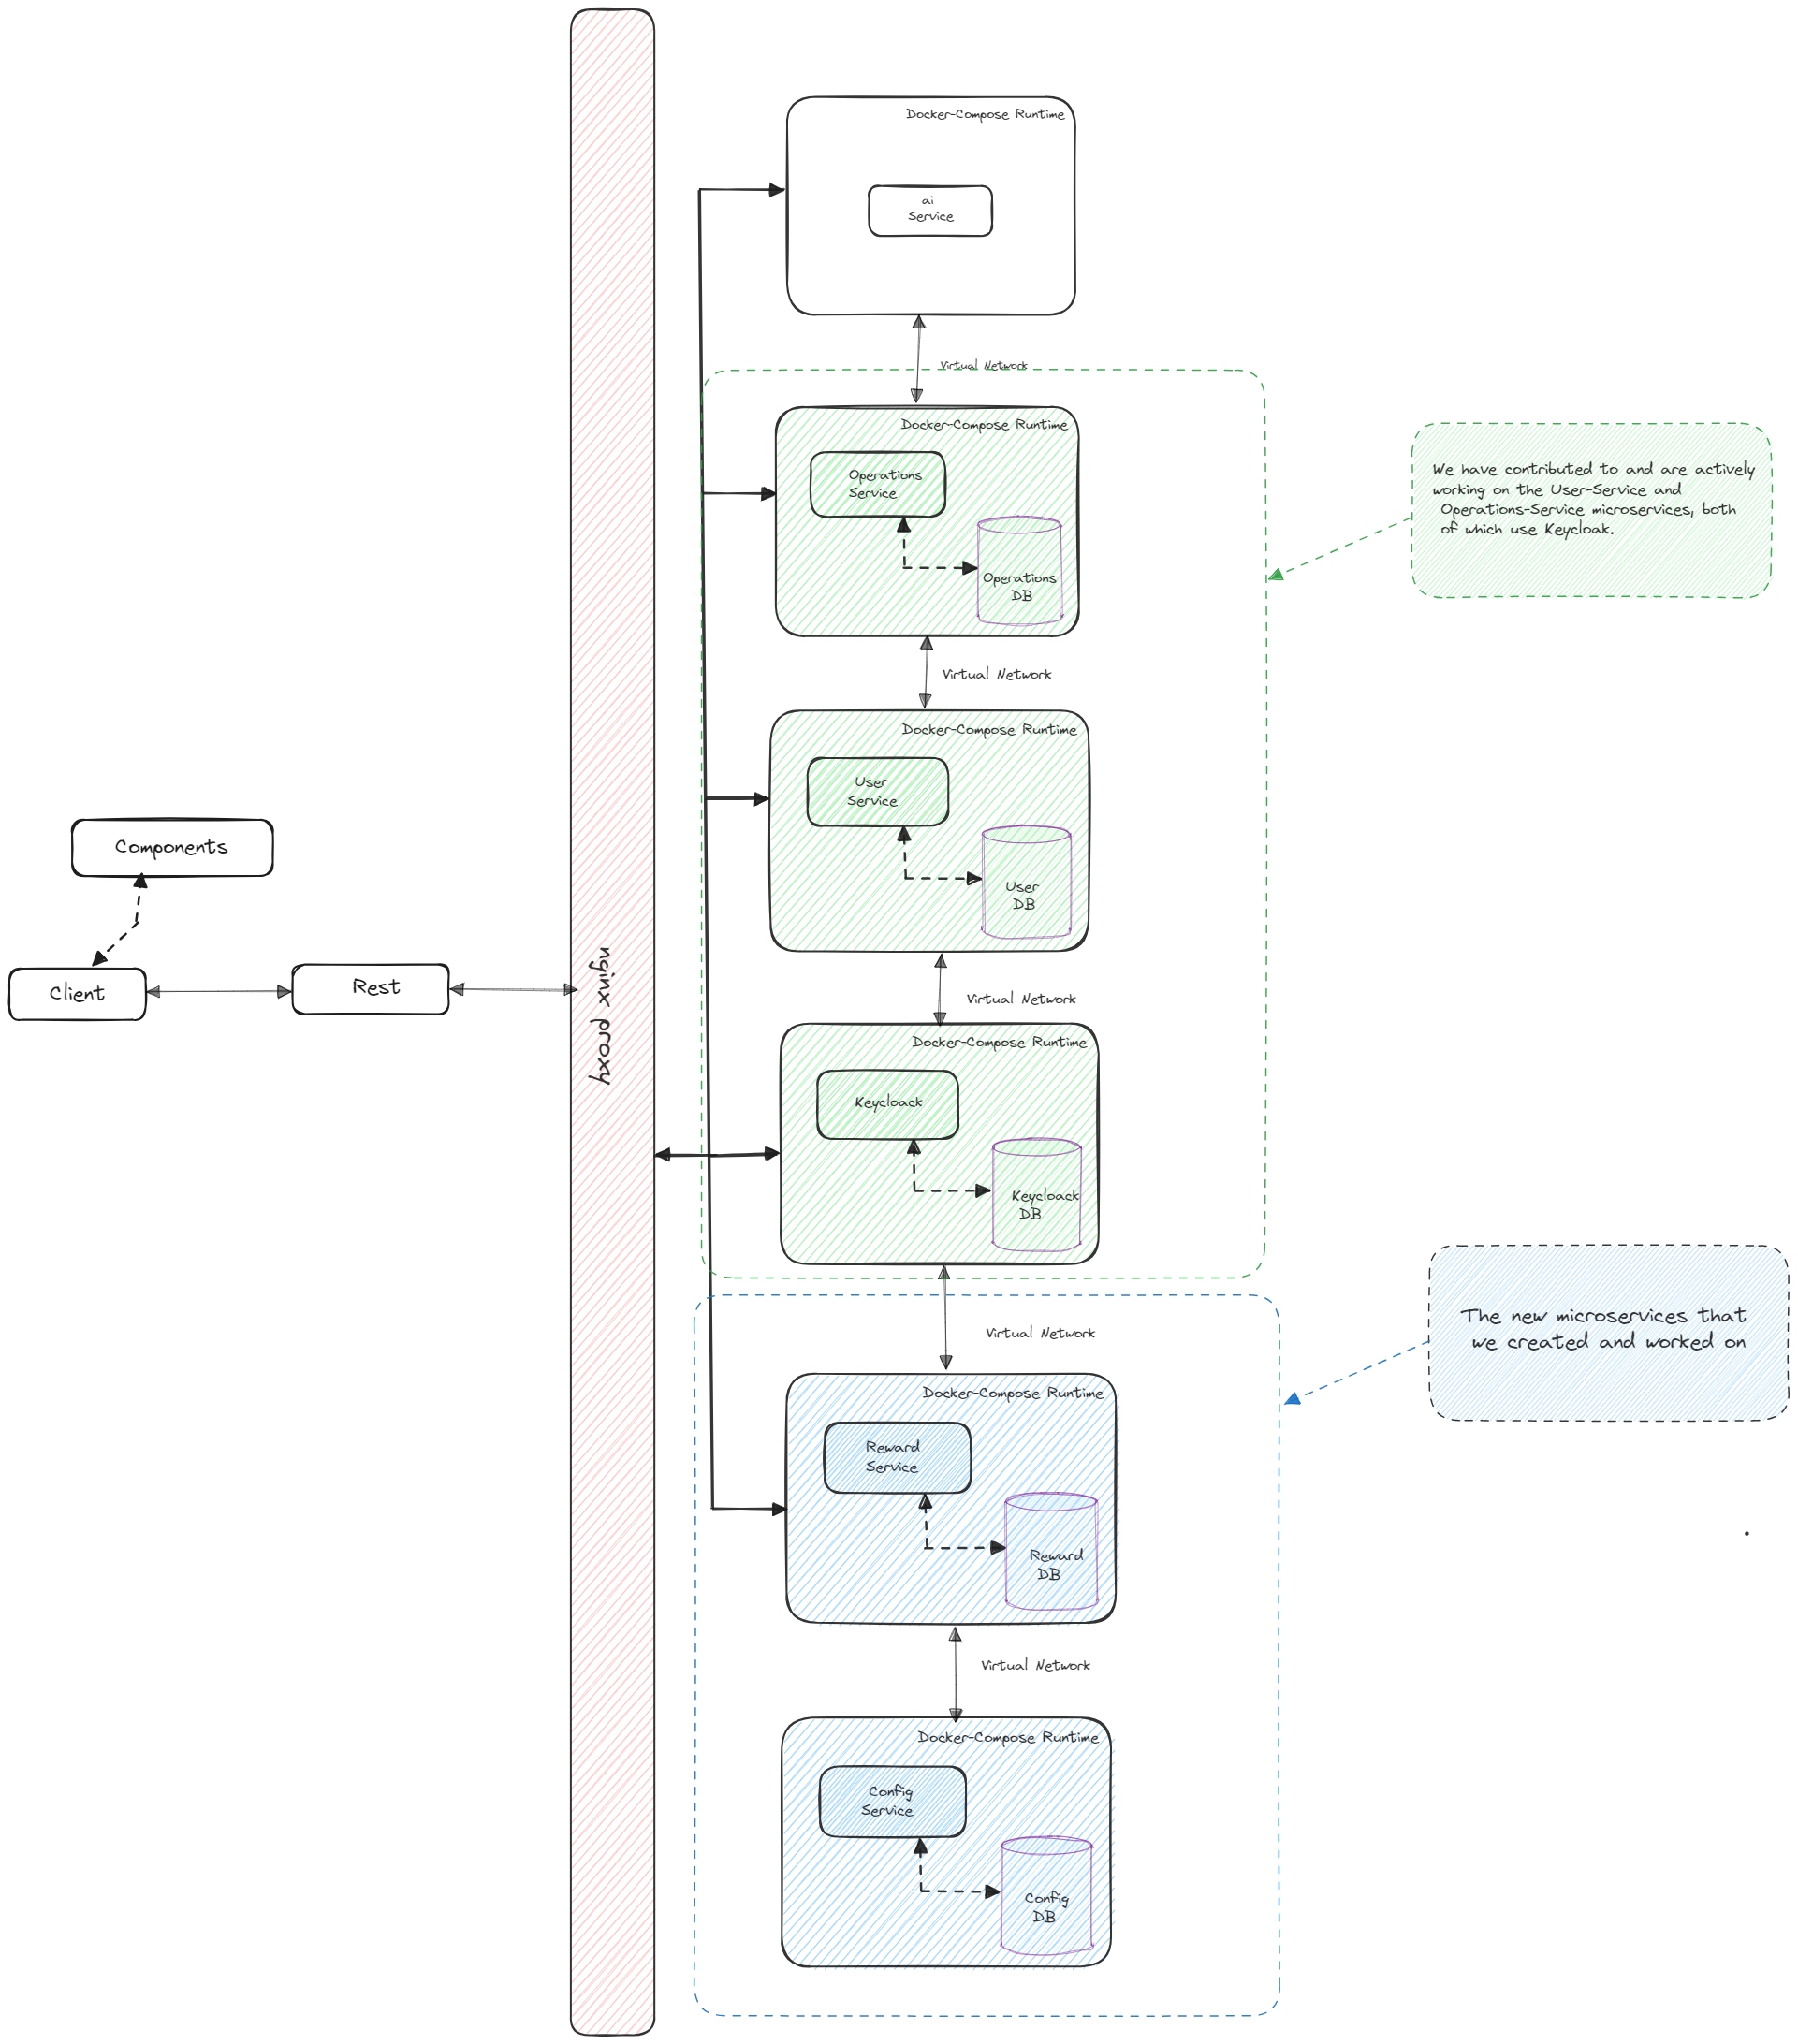
\includegraphics[width=1\textwidth]{src/assets/chapters/AermaxArchitecture.png}
    \caption{Aermax Architecture}
    \label{fig:aermax-architecture}
\end{figure}


\section{Technologies}
A project can always look simple from the outside, however if we dive deeply into how most software is made, we can see that it's not that simple of a process.
Therefore, this part will list all of the technologies that we've used and also some of the major technical difficulties we've encountered during the realization of our project.

\medskip

\begin{itemize}
    \item \textbf{Kubernetes:} \newline Kubernetes \cite{Kubernetes} is the most powerful tool for managing containerized workloads in the cloud. \newline
          \begin{minipage}{\linewidth}
              \centering
              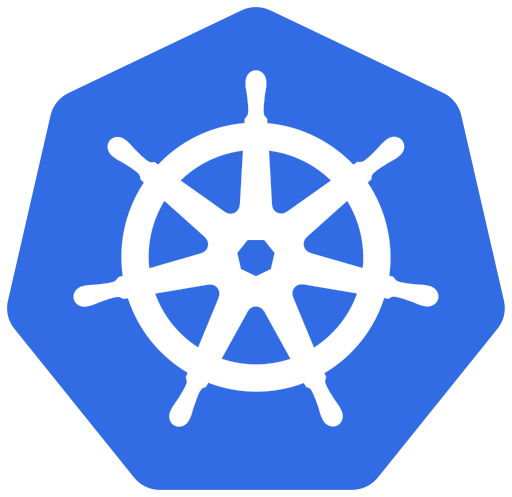
\includegraphics[width=3cm]{src/assets/logos/kubernetes_512x512.png}
              \captionof{figure}{Logo of Kubernetes}
          \end{minipage}
    \item \textbf{LaTeX:} \newline LaTeX \cite{latex-project} is a high-quality document preparation and typesetting system for technical grade documents. \newline \newline
          \begin{minipage}{\linewidth}
              \centering
              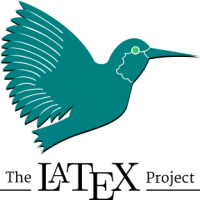
\includegraphics[width=3cm]{src/assets/logos/latex_200x200.png}
              \captionof{figure}{Logo of The LaTeX Project}
          \end{minipage}
    \item \textbf{Spring Boot:} \newline SpringBoot \cite{SpringBoot} is a powerful framework for building Java-based enterprise applications
. \newline \newline
          \begin{minipage}{\linewidth}
              \centering
              
\includegraphics[width=6.5cm]{src/assets/logos/Springboot.png}
              \captionof{figure}{Logo of Spring Boot}
          \end{minipage}
    \item \textbf{ReactJS:} \newline ReactJS \cite{ReactJS} is a JavaScript library for building user interfaces. \newline \newline
          \begin{minipage}{\linewidth}
              \centering
              
\includegraphics[width=3.5cm]{src/assets/logos/reactjs.png}
              \captionof{figure}{Logo of ReactJS}
          \end{minipage}
    \item \textbf{Keycloak:} \newline  Keycloak \cite{Keycloak} is an open-source identity and access management solution. \newline \newline
          \begin{minipage}{\linewidth}
              \centering
              
\includegraphics[width=6.5cm]{src/assets/logos/Keycloak-logo.png}
              \captionof{figure}{Logo of Keycloak}
          \end{minipage}
    \item \textbf{Python:} \newline  Python \cite{Python} is a versatile programming language used for various types of software development. \newline \newline
          \begin{minipage}{\linewidth}
              \centering
              
\includegraphics[width=6.5cm]{src/assets/logos/python.png}
              \captionof{figure}{Logo of Python}
          \end{minipage}
    \item \textbf{NestJS:} \newline NestJS \cite{NestJS} is a framework for building efficient, reliable, and scalable server-side applications. \newline \newline
          \begin{minipage}{\linewidth}
              \centering
              
\includegraphics[width=6.5cm]{src/assets/logos/nestjs_logo_icon.png}
              \captionof{figure}{Logo of NestJS}
          \end{minipage}
    \item \textbf{React Query:} \newline React Query \cite{ReactQuery} is a library for fetching, caching, and synchronizing server state in React applications. \newline \newline
          \begin{minipage}{\linewidth}
              \centering
              
\includegraphics[width=5.5cm]{src/assets/logos/react-query.png}
              \captionof{figure}{Logo of React Query}
          \end{minipage}
    \item \textbf{Langchain:} \newline Langchain \cite{Langchain} is a framework for developing applications powered by language models. \newline \newline
          \begin{minipage}{\linewidth}
              \centering
              \includegraphics[width=6.5cm]{src/assets/logos/langchain.png}
              \captionof{figure}{Logo of Langchain}
          \end{minipage}
\end{itemize}

\setcounter{secnumdepth}{0}
\section{Conclusion}
Defining and implementing these functional and technical requirements is crucial for developing a robust, reliable, and user-friendly Aermax application that meets the needs of our users and stakeholders, ensuring scalability, security, and comprehensive functionality.
\chapter{ Sprint 1 : Enhancements and Integrations}
\setcounter{secnumdepth}{0}

\section{Introduction}
In this chapter, we cover the first sprint of the Aermax project, focusing on the key enhancements and features we implemented to improve the platform.
\setcounter{secnumdepth}{2} 
\section{Major Features and Enhancements}
This section details the major features and enhancements introduced during the first sprint of the Aermax project. Each item listed in the sprint backlog was carefully selected to address critical needs and provide significant improvements to the platform's functionality and user experience.
\subsection{Sprint Backlog Detail}
Below is a detailed representation of our sprint backlog, showcasing the major tasks we committed to delivering in Sprint 1. We fixed around \textbf{26+ bugs, feature enhancements and new features }in Sprint 1. Below, we're going to share some of them. The biggest changes that we can discuss are highlighted below the blue colored line in the table.
\begin{longtable}{ | m{0.15\textwidth} | m{0.2\textwidth} | m{0.25\textwidth} | m{0.1\textwidth} | m{0.16\textwidth} | }
    \caption{Detailed Sprint Backlog} \\
    \hline
    \textbf{Type} & \textbf{Title} & \textbf{Description} & \textbf{Priority} & \textbf{Estimation} \\
    \hline
    \endfirsthead
    \hline
    \textbf{Type} & \textbf{Title} & \textbf{Description} & \textbf{Priority} & \textbf{Estimation} \\
    \hline
    \endhead
    \hline
    \endfoot
    \endlastfoot
    \rowcolor{blue!20} 
    Feature & Dynamic Equipment List & Develop a dynamic equipment list feature that organizes and manages equipment groups, ensuring each group and equipment item can be created, updated, and assigned to sub-companies and packets as needed. This feature aims to improve flexibility and ease of equipment management within the application. & High & 40h \\
    \hline
    \rowcolor{blue!20} Feature & Implement User Authentication System & Create a user authentication system enabling subcontractors to self-register, login, and manage passwords securely, allowing independent access to the platform's features. & High & 12h \\
    \hline
    \rowcolor{blue!20} 
    Enhancement & Adjust Feedback Notification & Enhance the feedback system to include notifications in Microsoft Teams, ensuring real-time updates . & Medium & 8h \\
    \hline
    Enhancement & Set Dynamic Project Status & Dynamically set project status based on packet statuses. & High & 5h \\
    \hline
    Enhancement & Add Field to User Edit & Include additional fields in the user edit form. & Medium & 2h \\
    \hline
    Feature & Set Default Calendar View & Remember last selection for default calendar view using localStorage. & Medium & 1h \\
    \hline
    Enhancement & Restrict Project Creation & Prevent subcontractors from creating new projects. & High & 1h \\
    \hline
    Enhancement & Remove Team Types & Remove unnecessary team types from the app to streamline functionality. & Low & 6h \\
    \hline
    Feature & Calendar View with New Filters & Implement new filters for the calendar view for better UX. & High & 40h \\
    \hline
    Feature & Implement Google Maps URL Generation & Generate Google Maps URLs for address visualization in subcompany user view. & Medium & 4h \\
    \hline
    Bug & Overhaul User Access Restrictions & Fix critical access restrictions and bugs for subcompany users. & High & 8h \\
    \hline
    \rowcolor{blue!20} 
    Feature & Overhaul the Role System & Revise the role system to clarify permissions and responsibilities. & High & 8h \\
    \hline
    Feature & Automate Username Generation & Auto-generate usernames during self-registration. & Medium & 16h \\
    \hline
    Feature & Remember Date Filters for Calendar & Implement a feature to remember date filters for the calendar. & Low & 3h \\
    \hline
    Feature & Overhaul the Project Status & Update project status features and adjust status enums and filters. & High & 3h \\
    \hline
    Bug & Fix Read-Only State of User Edit Form & Correct the issue with the user edit form being read-only for admins. & Medium & 4h \\
    \hline
    Bug & Remove Duplicate Aggregated Phases & Remove any duplicate instances of aggregated phases in the system. & High & 3h \\
    \hline
    \rowcolor{blue!20} Enhancement & Enhance Working Packets UI \& UX & Improve the UI and UX for working packets. & Medium & 16h \\
    \hline
\end{longtable}

\subsection{Dynamic Equipment List}
To effectively transition from a static to a dynamic equipment list, we need to carefully design the system architecture.

\subsubsection{Dynamic Equipment List Issues}
The Dynamic Equipment List feature was previously implemented as a static list, which required manual updates and did not reflect real-time changes to the equipment database. The key characteristics and drawbacks of the static implementation are outlined below:

\paragraph{Key Characteristics of the Static Implementation}
\begin{itemize}
    \item \textbf{Manual Updates:} The equipment list required manual updates.
    \item \textbf{Limited Flexibility:} The static list lacked flexibility and responsiveness to changes.
    \item \textbf{High Maintenance Overhead:} Frequent updates resulted in high maintenance overhead.
\end{itemize}

\paragraph{Drawbacks of the Static Implementation}
\begin{itemize}
    \item \textbf{Scalability:} As the number of equipment items grew, maintaining the static list became increasingly cumbersome.
    \item \textbf{Real-time Updates:} Changes to the equipment database were not immediately reflected in the list, leading to potential inconsistencies.
    \item \textbf{User Experience:} Users could not rely on the list for up-to-date information, impacting their ability to make informed decisions.
\end{itemize}

As illustrated in Figure \ref{fig:static_equipment_list}, subcontractors were limited to only checking the checkboxes for the available equipment.

\begin{figure}[H]
    \centering
    \resizebox{1\textwidth}{!}{
        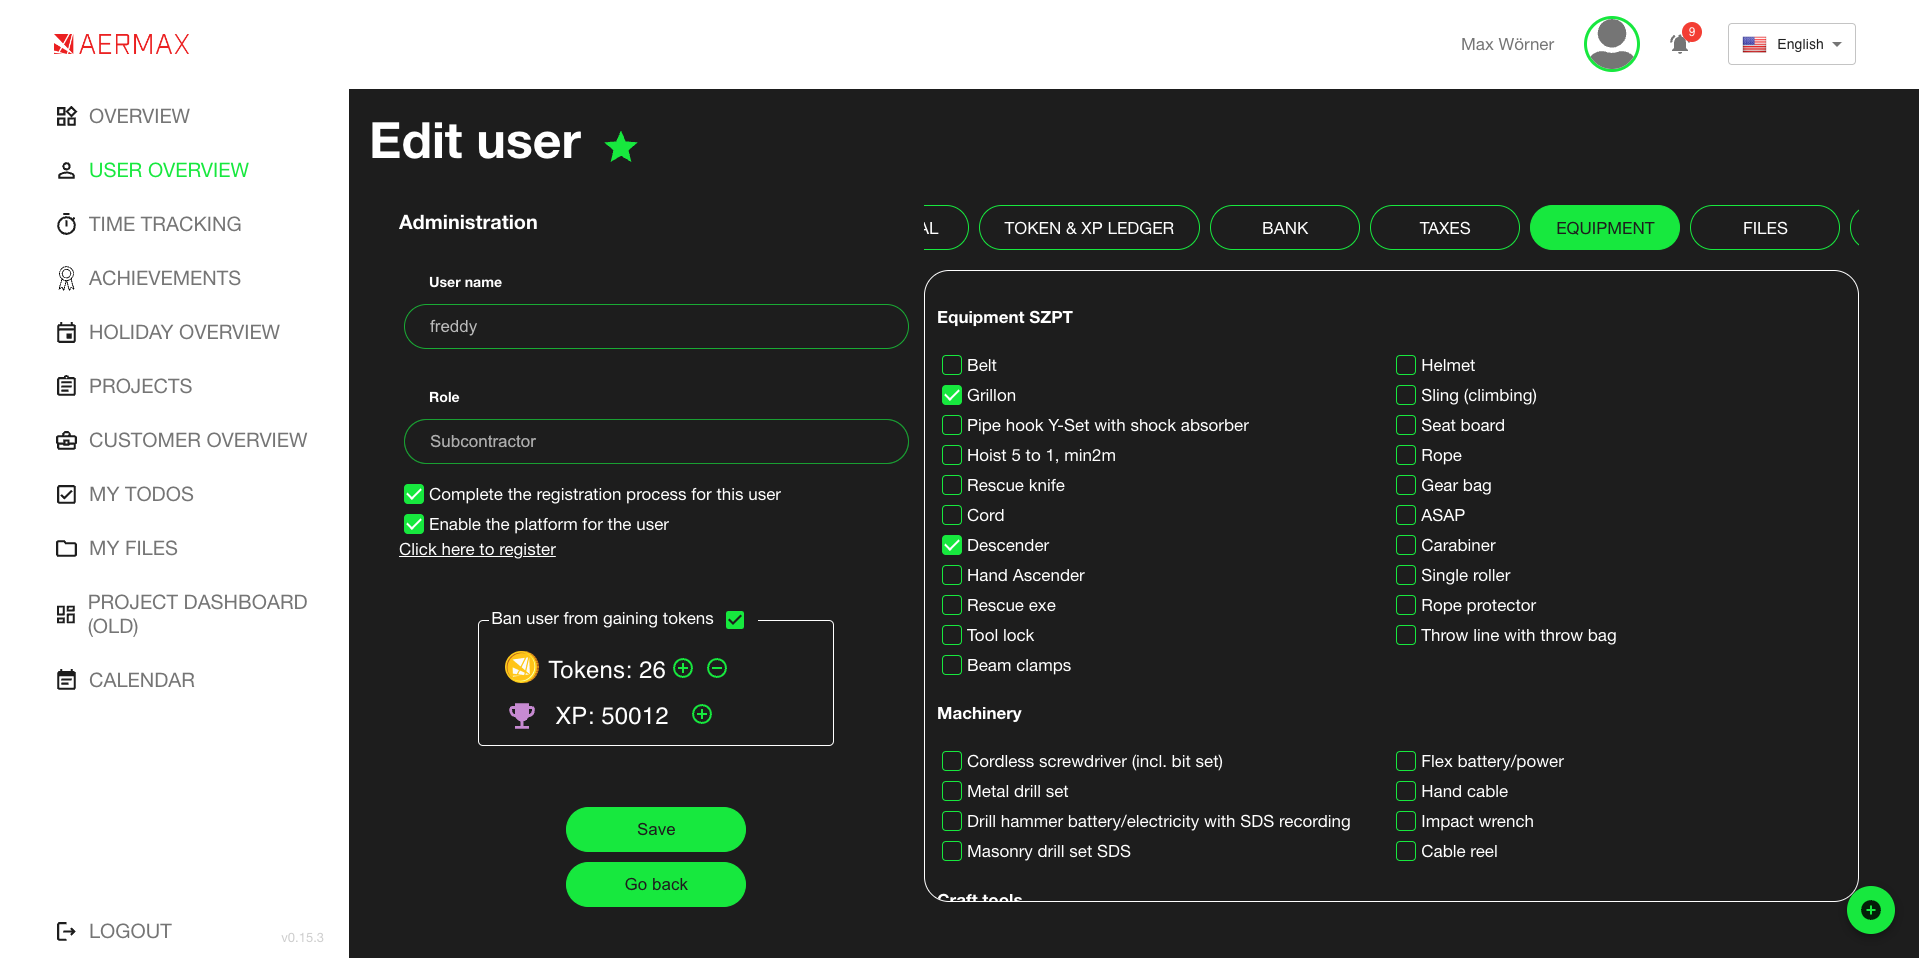
\includegraphics{src/assets/chapters/StaticDynamicEquipementList.png}
    }
    \caption{Previous Static Equipment List}
    \label{fig:static_equipment_list}
\end{figure}

\subsubsection{Dynamic Equipment List solution}
To address these issues, we are transitioning to a dynamic equipment list. The dynamic implementation will automatically update the list based on changes in the equipment database, ensuring real-time accuracy and reducing maintenance overhead. Key features of the dynamic implementation include:
\begin{itemize}
    \item \textbf{Real-time Updates:} The list will automatically reflect changes made to the equipment database.
    \item \textbf{Improved Scalability:} The system can handle an increased number of equipment items without additional maintenance.
    \item \textbf{Enhanced User Experience:} Users will have access to up-to-date information, improving their ability to make decisions.
    \item \textbf{Reduced Maintenance:} Eliminates the need for manual updates, reducing the time and effort required to maintain the list.
    \item \textbf{Request System:} Subcontractors can request new equipment items directly through the system, allowing admins to approve, reject, and assign these items to appropriate groups.
\end{itemize}

The planned dynamic equipment list will also include comprehensive admin and subcompany views. As shown in Figure \ref{fig:dynamic_equipment_list_admin}, admins will have the capability to create groups, assign equipment, move equipment, and approve or reject equipment requests. Subcontractors, as illustrated in Figure \ref{fig:dynamic_equipment_list_subcompany}, will be able to write and request new equipment items, ensuring they have the necessary tools for their projects.

\begin{figure}[H]
    \centering
    \resizebox{1\textwidth}{!}{
        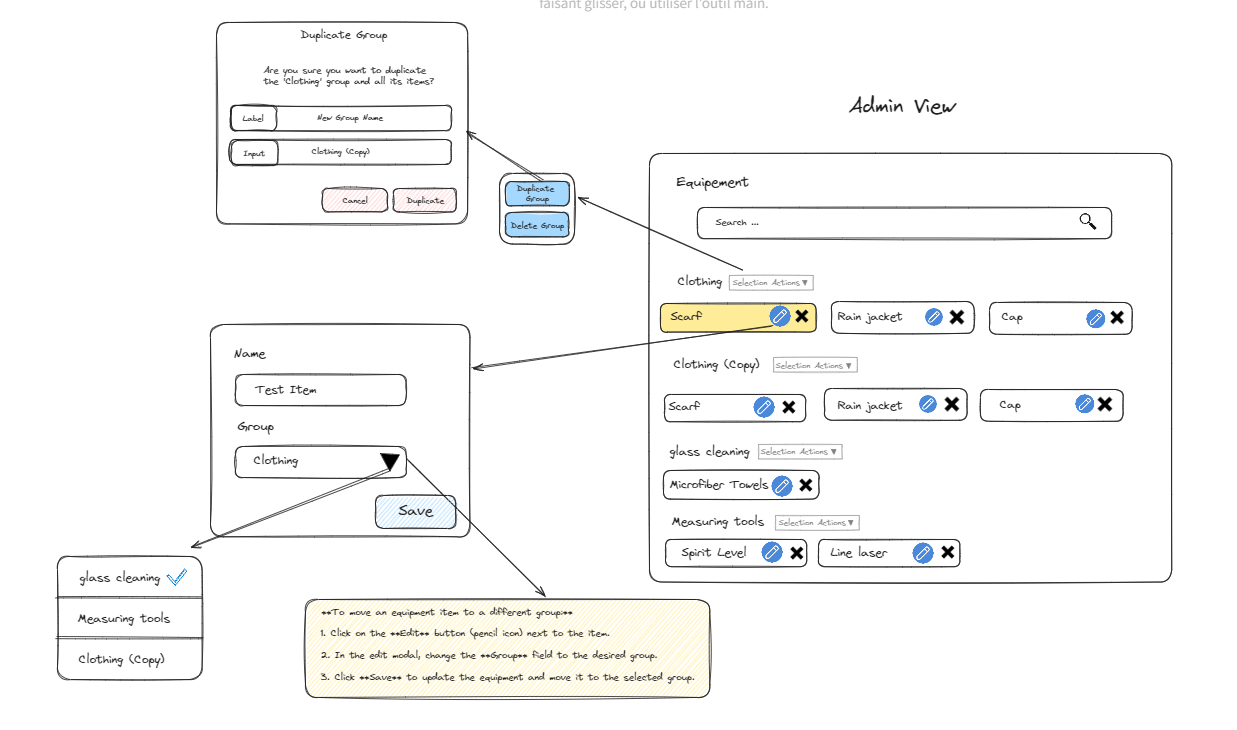
\includegraphics{src/assets/chapters/DynamicEquipementAdmin.PNG}
    }
    \caption{Planned Dynamic Equipment List - Admin View}
    \label{fig:dynamic_equipment_list_admin}
\end{figure}

\begin{figure}[H]
    \centering
    \resizebox{1\textwidth}{!}{
        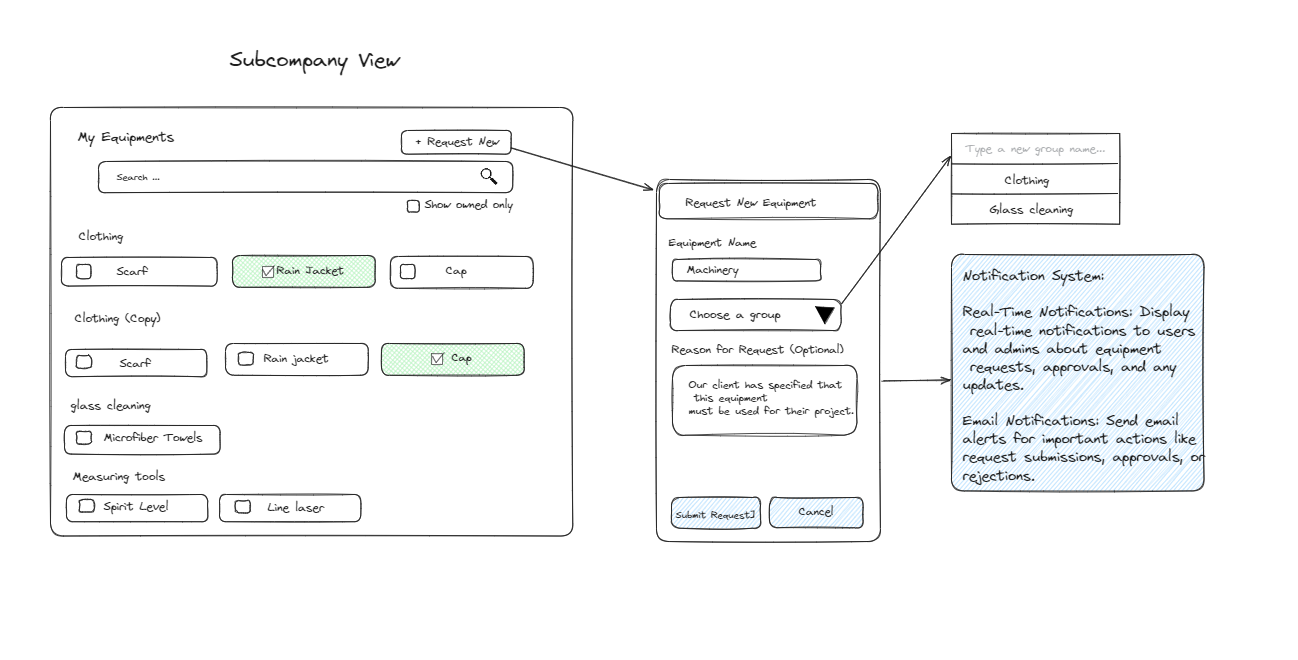
\includegraphics{src/assets/chapters/DynamicEquipementSubcompany.PNG}
    }
    \caption{Planned Dynamic Equipment List - Subcompany View}
    \label{fig:dynamic_equipment_list_subcompany}
\end{figure}

\subsubsection{Dynamic Equipment Design}
To effectively transition from a static to a dynamic equipment list, we need to carefully design the system architecture. The dynamic system will facilitate real-time updates, scalability, and a user-friendly experience. The following sections provide a detailed overview of the class structure and interactions essential for implementing this dynamic equipment list.

The dynamic equipment list system will consist of several key components:

\begin{itemize}
    \item \textbf{Equipment Class:} This class will represent individual equipment items, including attributes such as name, group, status (requested, approved, rejected), and other relevant details.
    \item \textbf{Group Class:} This class will manage groups of equipment, allowing the creation, duplication, and deletion of groups. It will also handle the assignment and movement of equipment items between groups.
    \item \textbf{Request Class:} This class will handle equipment requests submitted by subcontractors. It will track the status of requests (pending, approved, rejected) and include details such as the equipment name and requested group.
    \item \textbf{User Class:} This class will manage user information, differentiating between admin and subcontractor roles, and providing appropriate permissions and functionalities for each role.
    \item \textbf{Notification System:} This component will handle real-time and email notifications to keep users informed about important actions like equipment requests, approvals, and rejections.
\end{itemize}
\paragraph{Class Diagram}
The class diagram below (Figure \ref{fig:class_diagram}) illustrates the key components and relationships involved in the dynamic equipment list feature.
\begin{figure}[H]
    \centering
    \resizebox{1\textwidth}{!}{
        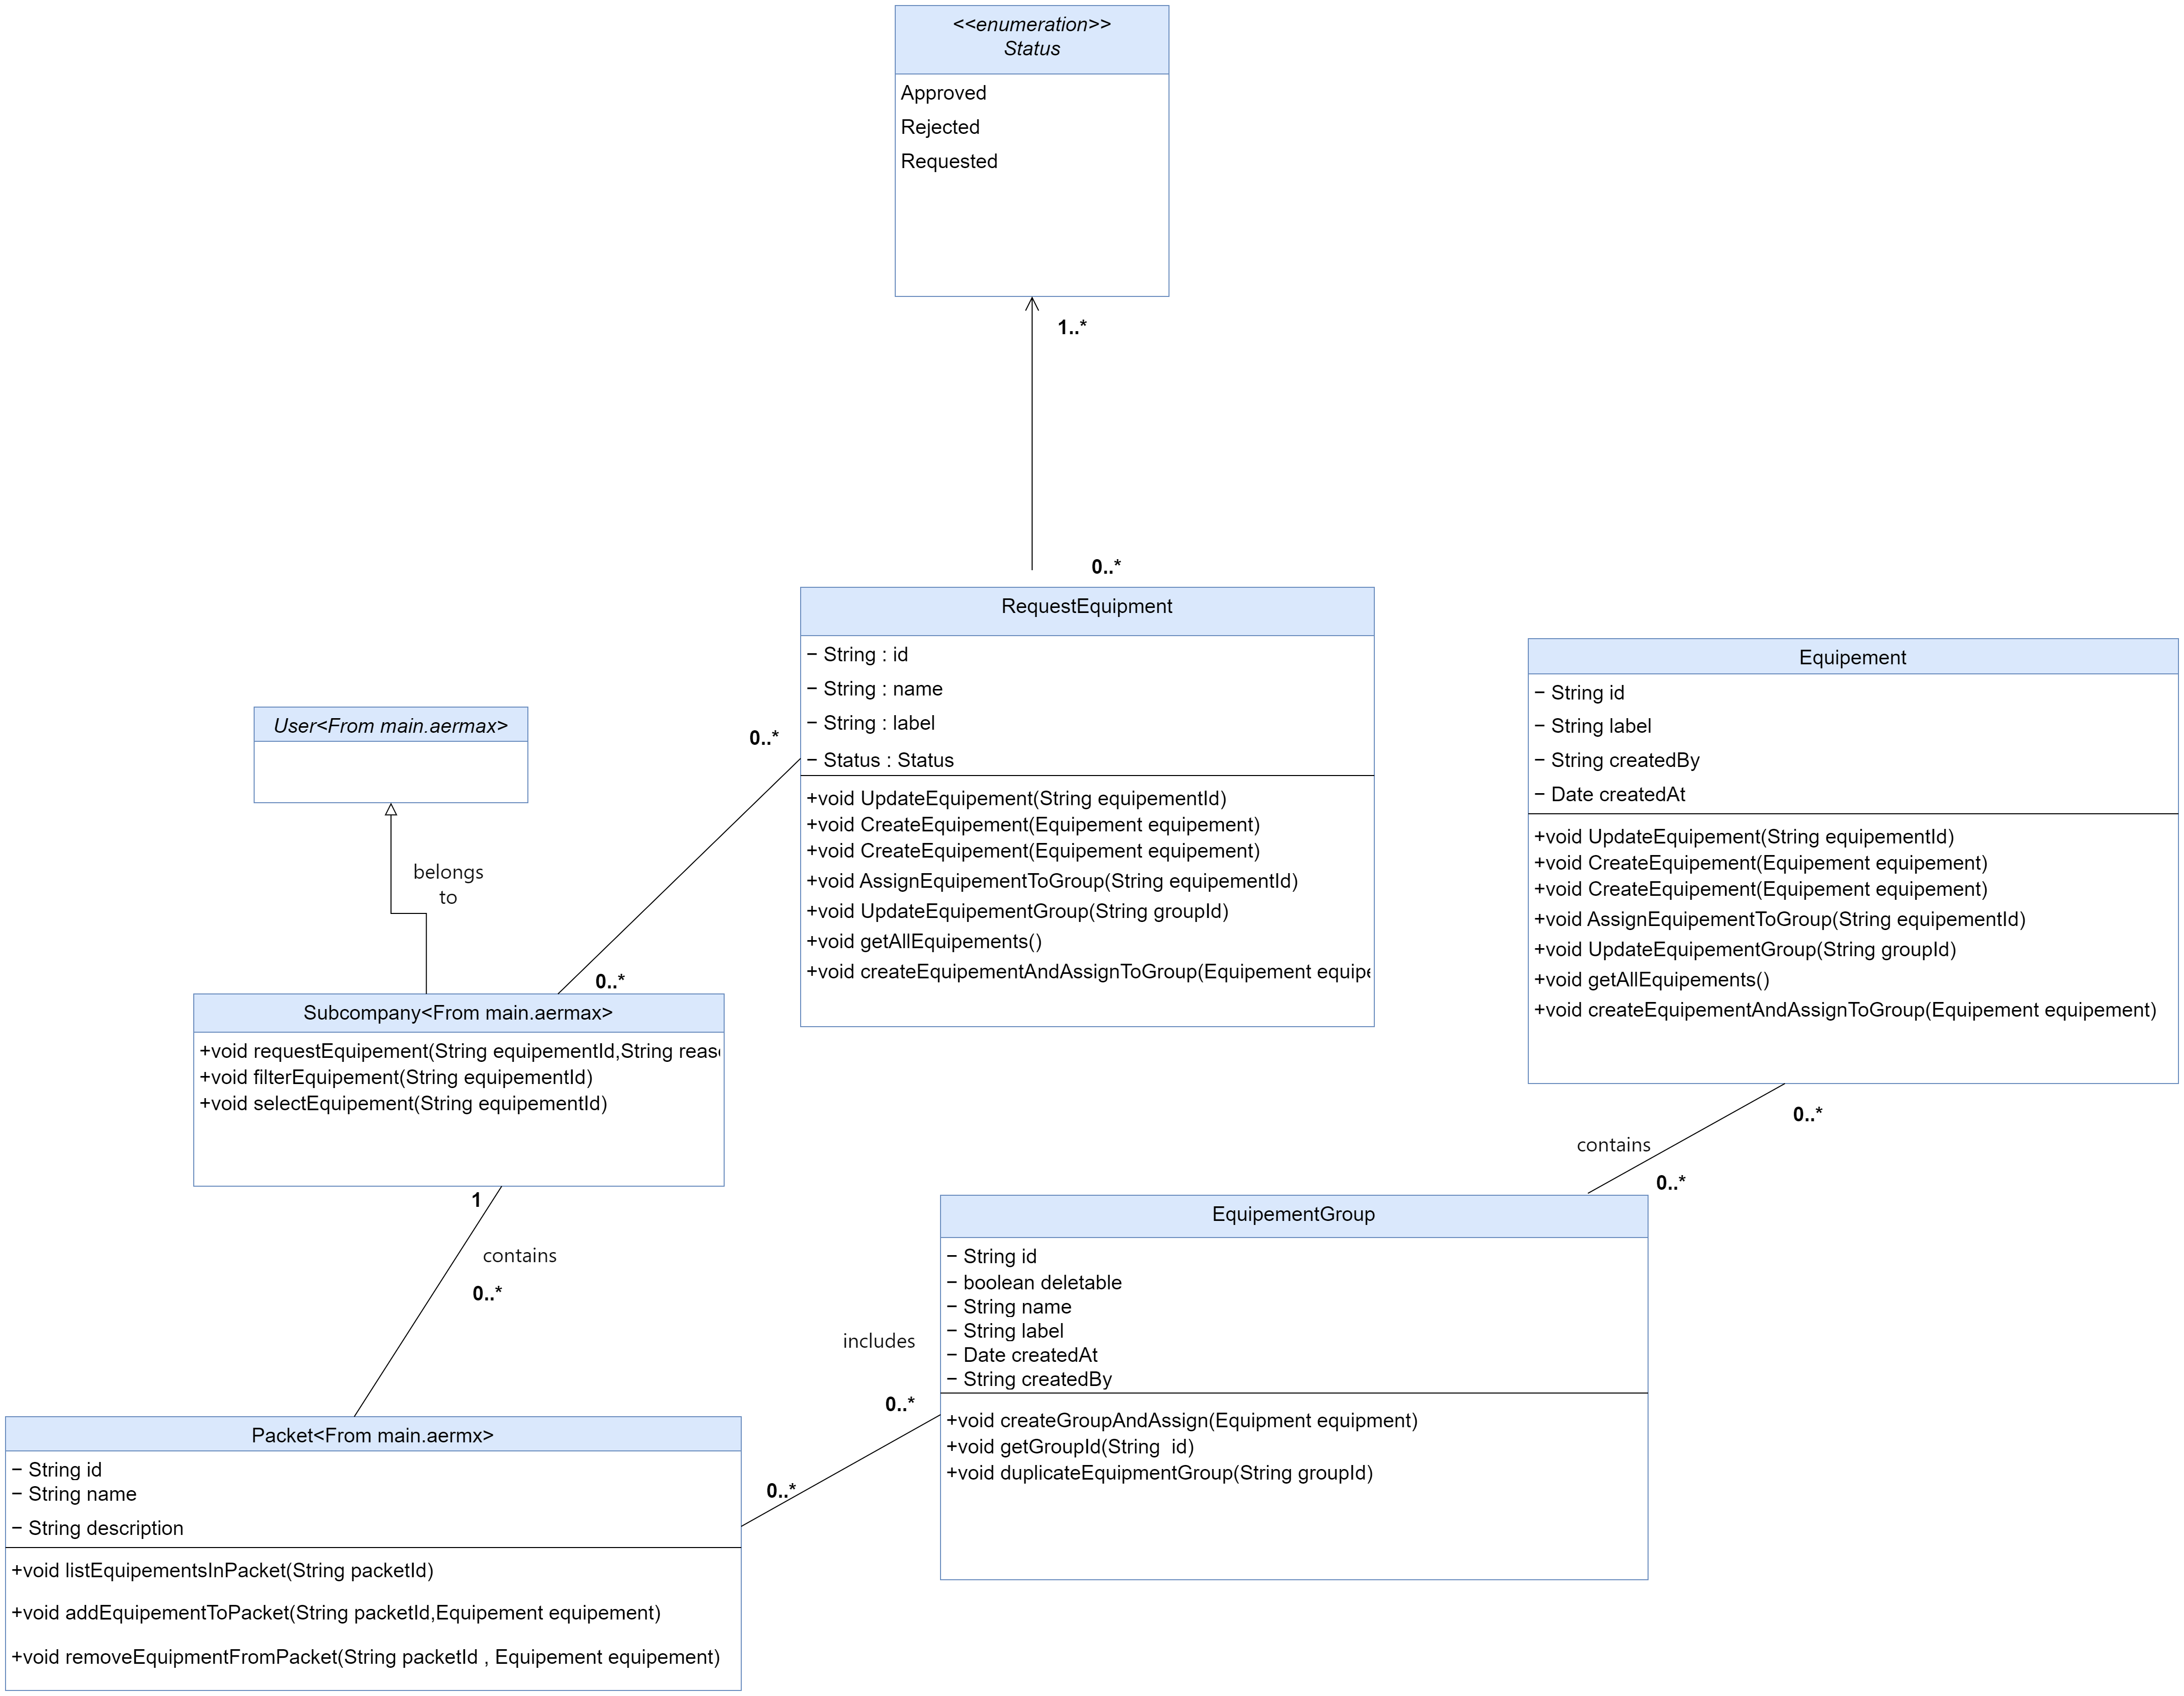
\includegraphics{src/assets/diagrams/DynamiEquipementListPng.png}
    }
    \caption{Class Diagram for Dynamic Equipment List}
    \label{fig:class_diagram}
\end{figure}


\paragraph{Subcompany Interface}
The images below show the subcompany interface after the implementation of the dynamic equipment list, illustrating the improved user experience for subcompany users.

\begin{figure}[H]
\centering
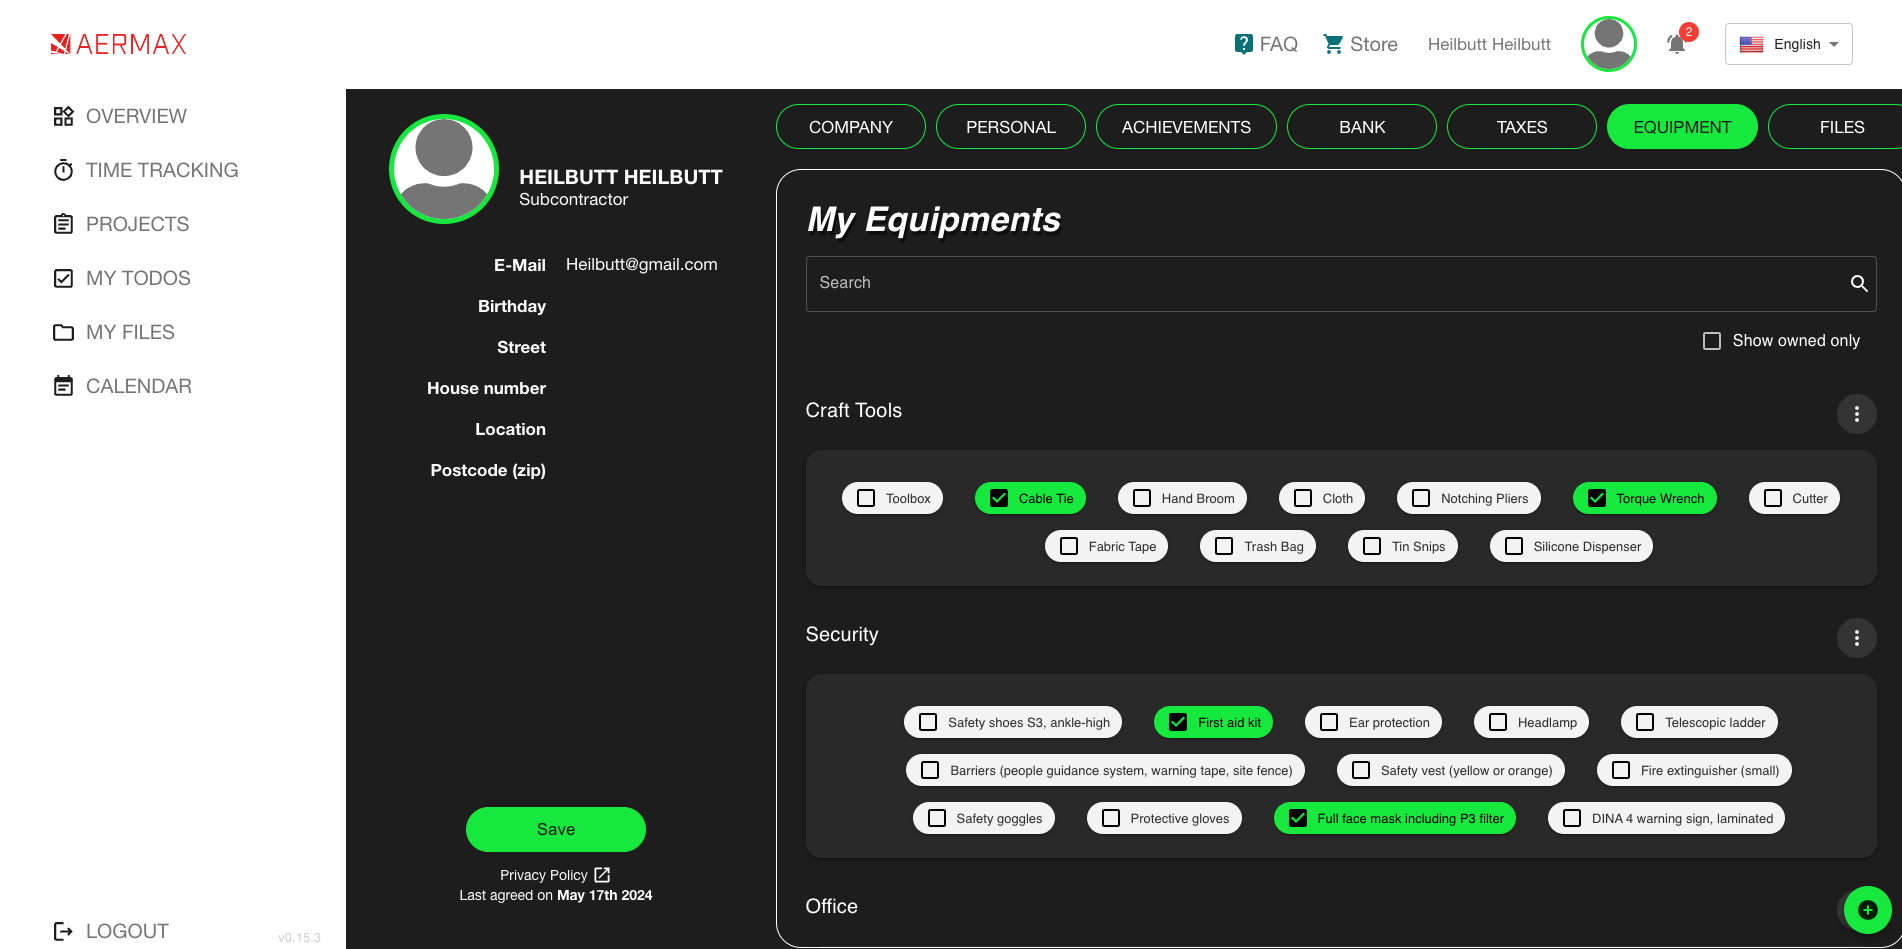
\includegraphics[width=0.9\textwidth]{src/assets/images/Interface1.png}
\caption{Subcompany Interface - Viewing Assigned Equipment}
\label{fig:subcompany_interface_1}
\end{figure}

\subsection{Adjust Feedback Notification}
To enhance the feedback feature, we plan to implement a system that allows administrators to send feedback notifications directly to Microsoft Teams. This feature aims to streamline communication and ensure that feedback is promptly addressed. The following sections outline the implementation strategy for this feature.

The feedback system will consist of several key components:

\begin{itemize}
    \item \textbf{Feedback Form:} The user interface where administrators can submit feedback. The form will include options for categorizing the feedback (Error, Incomprehensible, Unwanted Behavior, Miscellaneous) and a text area for detailed descriptions.
    \item \textbf{Feedback Database:} A storage system to save feedback entries. Each entry will include the feedback category, description, and a timestamp.
    \item \textbf{Notification Service:} A backend service that processes feedback entries and sends notifications to Microsoft Teams. This service will be designed to be extendable, allowing for future integration with other communication channels such as Slack or email.
\end{itemize}

\paragraph{Implementation Steps}
\begin{enumerate}
    \item \textbf{Feedback Form UI:} Enhance the existing feedback form (Figure \ref{fig:feedback_form}) to include the necessary fields and submission button. Ensure the form captures the feedback category and description.
    \item \textbf{Database Integration:} Create or update the database schema to store feedback entries. Each entry should capture the feedback category, description, and a timestamp.
    \item \textbf{Notification Service:} Develop a backend service that listens for new feedback entries in the database. Upon detecting a new entry, the service will format the feedback and send it as a notification to a designated Microsoft Teams channel.
    \item \textbf{Microsoft Teams Integration:} Use the Microsoft Teams API to send notifications. Ensure the notifications include all relevant feedback details and are formatted for readability.
\end{enumerate}

The following image (Figure \ref{fig:feedback_form}) illustrates the user interface for submitting feedback.

\begin{figure}[H]
    \centering
    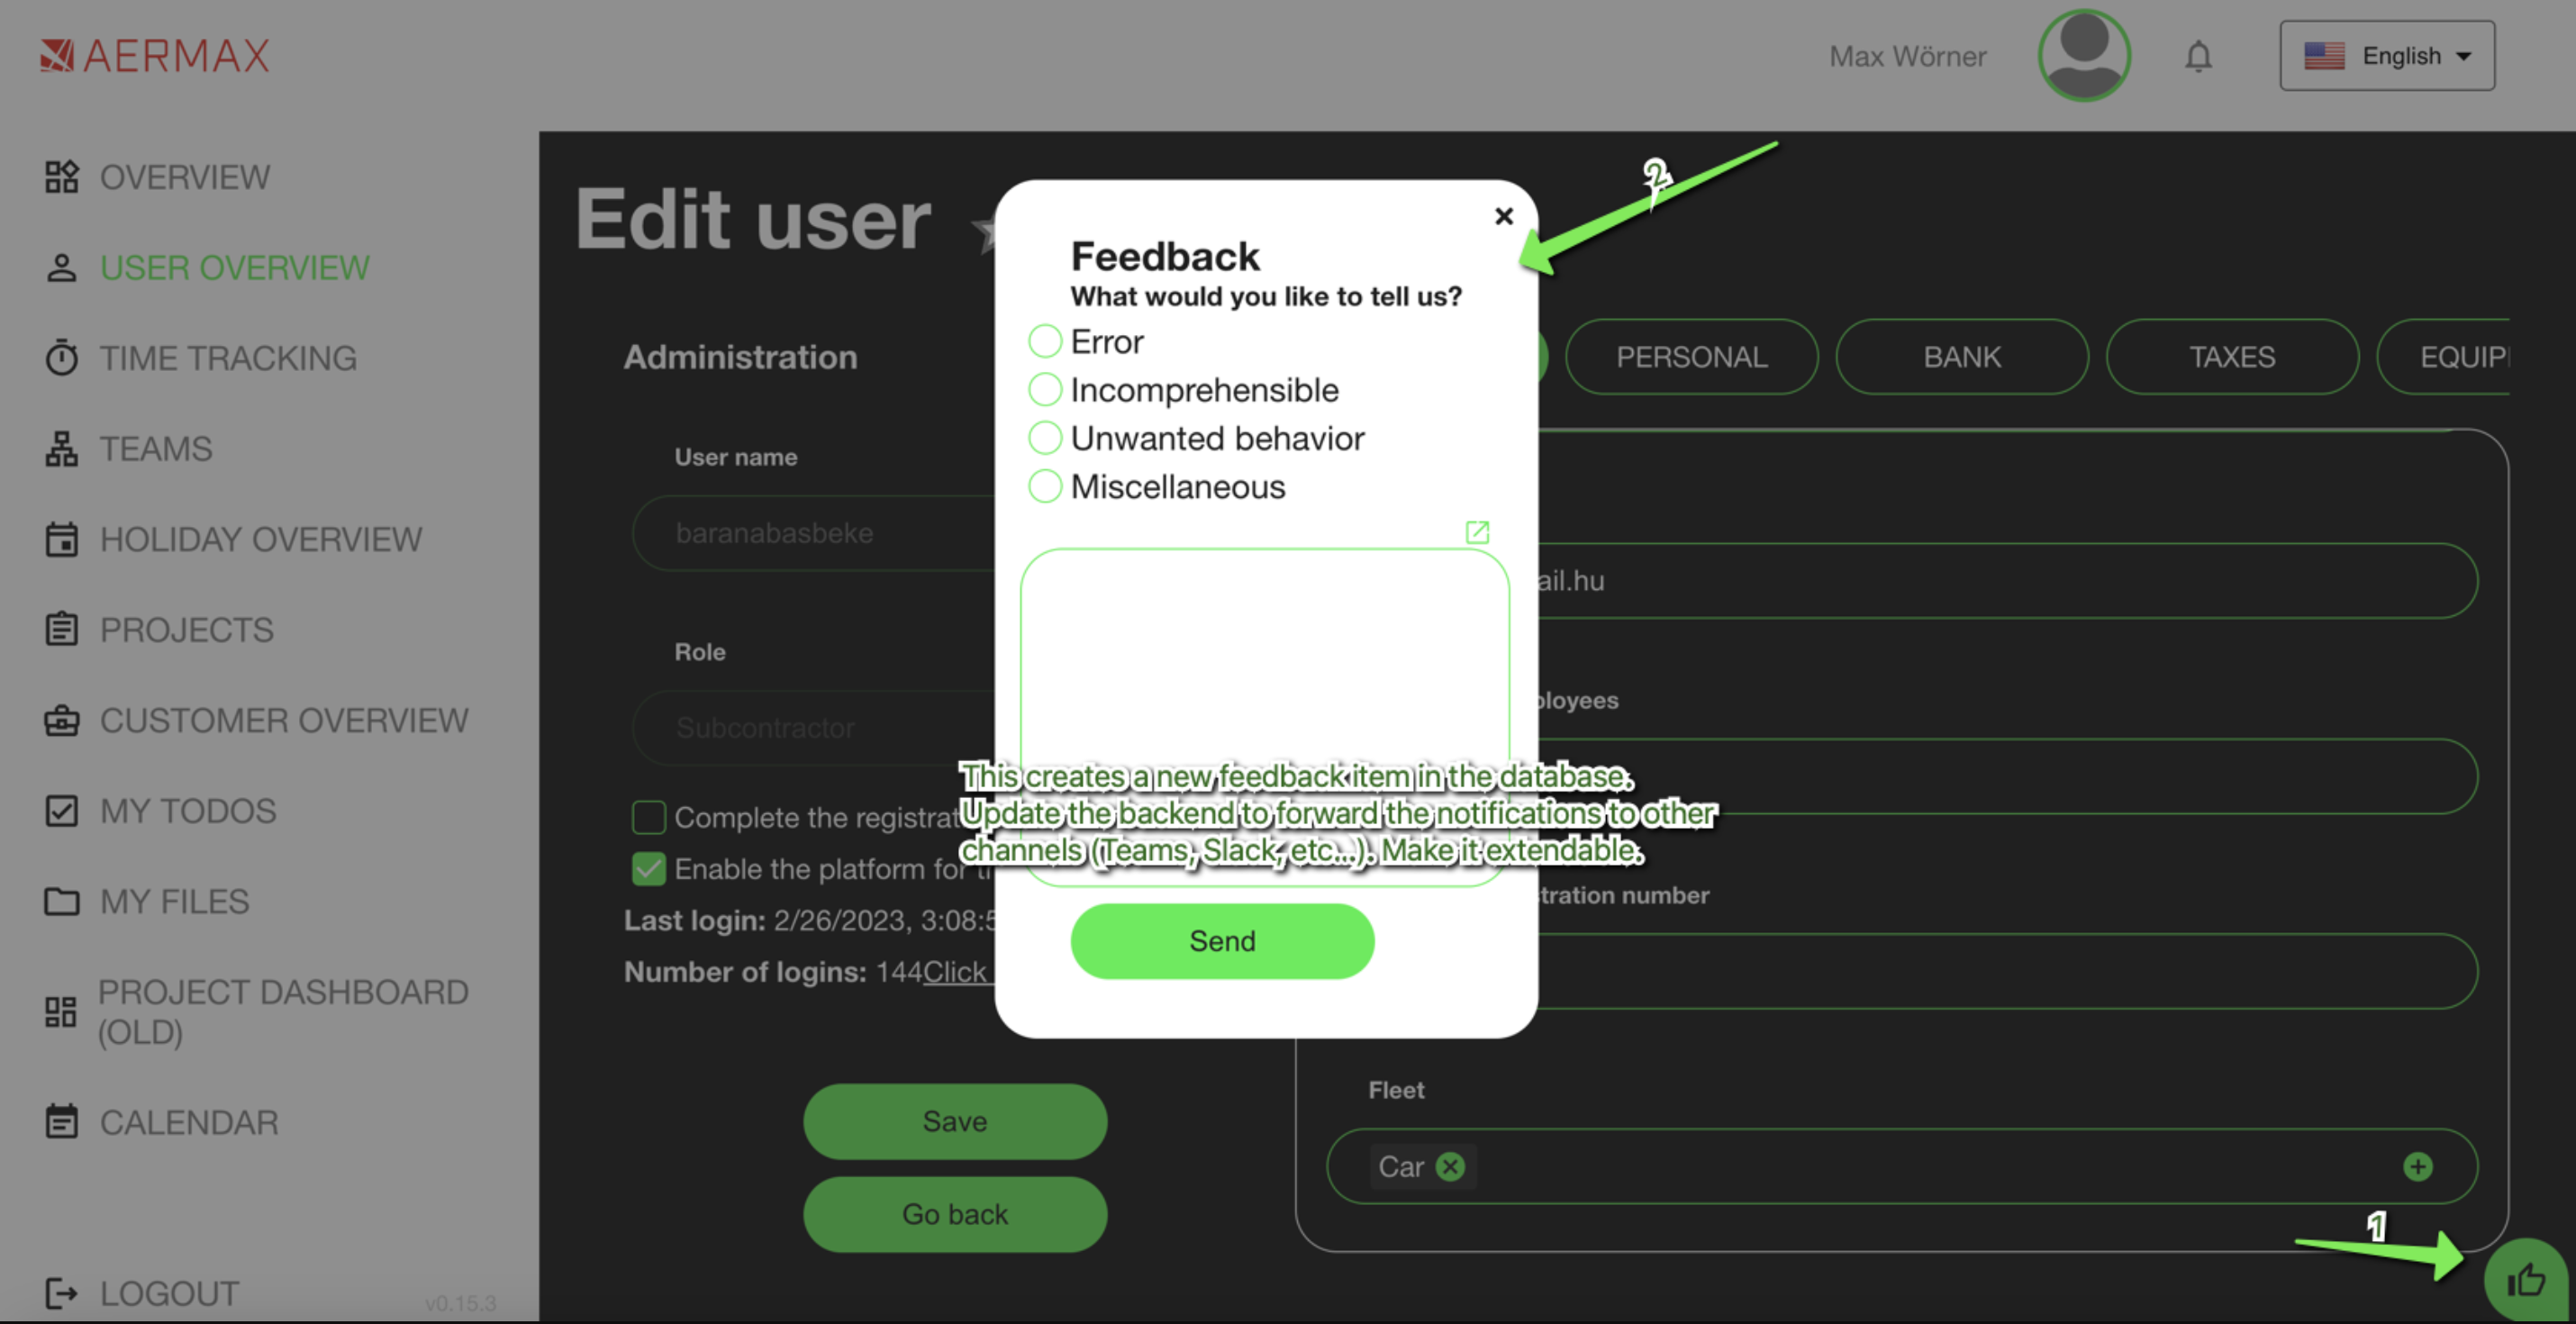
\includegraphics[width=1\textwidth]{src/assets/images/TeamsNotification.png}
    \caption{Feedback Form and Notification}
    \label{fig:feedback_form}
\end{figure}

\subsection{Overhaul of the Role System}
The Aermax platform's role system was overhauled during Sprint 1 to improve clarity and security. Previously, roles had overlapping permissions, causing confusion and security issues. Now, each role has specific permissions aligned with its responsibilities.

\subsubsection{Detailed Role Permissions Before \& After}
\begin{longtable}{|p{3cm}|p{5cm}|p{5cm}|}
\caption{Comparison of role permissions before and after the overhaul.} \label{tab:role_permissions_comparison} \\
\hline
\textbf{Role} & \textbf{Permissions Before Overhaul} & \textbf{Permissions After Overhaul} \\ \hline
\endfirsthead

\multicolumn{3}{c}%
{{\bfseries Table \thetable\ Continued from previous page}} \\
\hline
\textbf{Role} & \textbf{Permissions Before Overhaul} & \textbf{Permissions After Overhaul} \\ \hline
\endhead

\hline \multicolumn{3}{|r|}{{Continued on next page}} \\ \hline
\endfoot

\hline
\endlastfoot

Administrator & 
- Limited access to projects managed by non-admin Project Managers &
- Full access to all projects \\ \hline

Worker & 
- Could see all project packets &
- Can only see their own projects and packets \\ \hline


Team Leader & 
- Could see only their own packets &
- Can see packets of other workers within their phase   \\ \hline

\end{longtable}

\textbf{Scenario Demonstrations After Overhaul:}
\begin{itemize}
    \item \textbf{Administrator Scenario:} An Administrator maintains complete control, capable of managing all aspects of the project lifecycle.
    \item \textbf{Project Manager Scenario:} Project Managers are now provided with tailored access, capable of managing specific project packets and workflows.
    \item \textbf{Worker Scenario:} Workers are limited to their own packets, focusing their dashboard on personal tasks without additional project creation or overview privileges.
    \item \textbf{Team Leader Scenario:} Team Leaders have targeted oversight, managing only the packets within their project phase, without the distraction of other project overviews or creation capabilities.
\end{itemize}
This targeted approach in the role system refines the user experience on the Aermax platform, ensuring each role has the access needed to perform effectively, securely, and efficiently.

\subsection{Enhance Working Packets UI \& UX}
In our continuous efforts to elevate the user experience on the Aermax platform, a significant upgrade was made to the Working Packets UI \& UX, particularly focusing on the administrative interface. Key improvements include:

\begin{itemize}
    \item Alleviating the difficulties the admin faced in managing packets.
    \item Addressing the need to duplicate each packet individually when 30 packets needed duplication in one day.
    \item Developing a new interface presented as a table.
    \item Allowing the admin to duplicate multiple packets simultaneously.
    \item Offering more filtering functionalities.
    \item Providing an improved, user-friendly view.
\end{itemize}

See the implemented feature in Figure \ref{fig:ui_ux_enhancements}.

\begin{figure}[H]
    \centering
    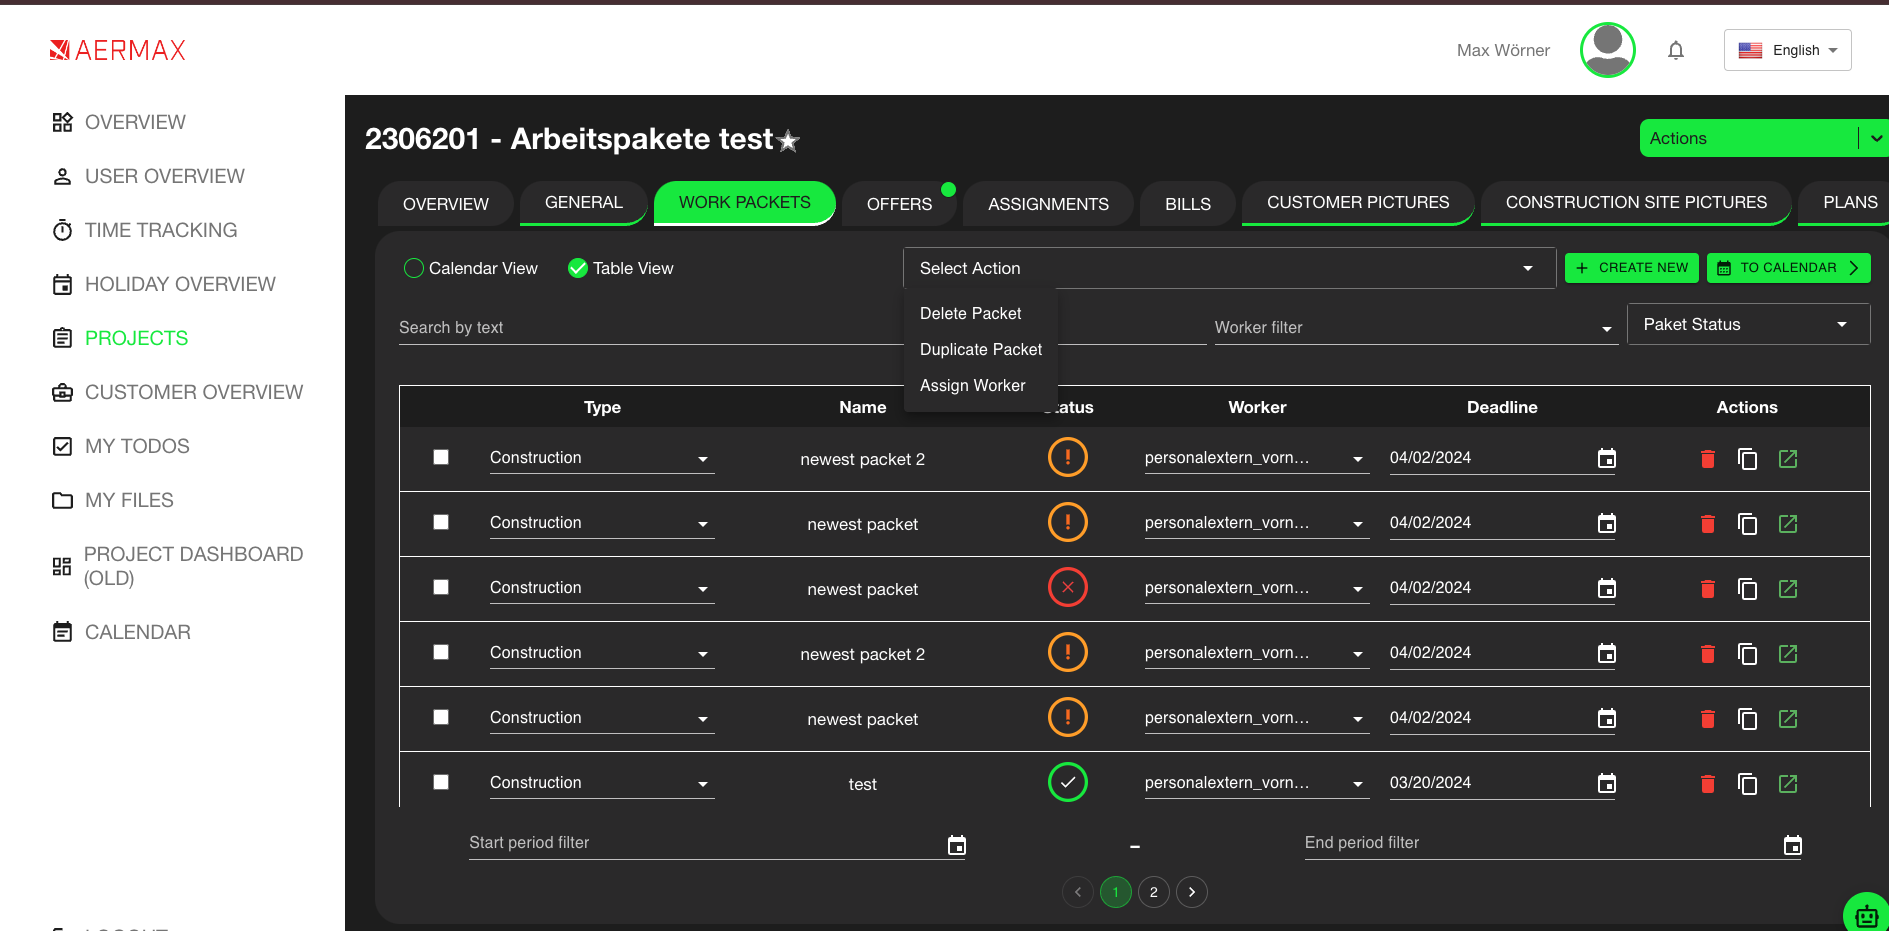
\includegraphics[width=0.9\textwidth]{src/assets/chapters/newTable2.png}
    \caption{Sketch of Planned UI/UX Enhancements for Working Packets}
    \label{fig:ui_ux_enhancements}
\end{figure}

\subsection{User Authentication System}
We implemented an authentication system using Keycloak. As part of this overhaul, we encountered the challenge of duplicate user entries due to previous system design limitations. By leveraging Keycloak’s versatile user federation and identity provider features, we were able to consolidate user accounts and eliminate redundancies, thereby solving the issue of duplicate entries. Keycloakify complemented this integration by allowing us to customize the authentication pages to align with our platform's aesthetics and usability standards.

\subsubsection{Feature Implementation Table:}
\begin{table}[H]
\centering
\begin{tabularx}{\textwidth}{|X|X|X|}
\hline
\textbf{Feature} & \textbf{Technology Implemented} & \textbf{Description} \\
\hline
Login/Signup & Keycloak, Keycloakify & Integrated with Keycloak to secure and streamline user access, enhanced by Keycloakify for customized UI/UX. \\
\hline
Password Management & Keycloak & Developed a secure and user-friendly password management system, providing users with ease of control over their credentials. \\
\hline
\end{tabularx}
\caption{Summary of Keycloak feature implementations.}
\label{tab:keycloak_features}
\end{table}

\setcounter{secnumdepth}{0}
\section{Conclusion}
Sprint 1 has laid a strong foundation for the Aermax platform by addressing critical needs and improving overall functionality and user experience. Looking ahead to Sprint 2, we will focus on a major feature: the reward system, which promises to further enhance user engagement and satisfaction.


\chapter{Sprint 2: Reward System}
\minitoc
\newpage

\setcounter{secnumdepth}{0} % Set the section counter to 0 so next section is not counted in toc
% ----------------------- Introduction ----------------------- %
\section{Introduction}
Throughout this chapter, we will delve into the planning, design considerations, and implementation of our reward system, from conception and development to deployment.
\section{Sprints Backlog}
During the Sprint Planning meeting, the effort for each task in the first and second sprint backlogs was assessed based on the total working hours required. The prioritization of these backlog items is depicted through their sequence in the table, with items placed at the top representing higher urgency. Additionally, the accompanying image showcases the board that serves as our operational platform at Incedo.

% \begin{figure}[H]
%     \centering
%     \includesvg[width=1.55\textwidth]{src/assets/chapters/reward-system-backloog.svg}
%     \caption{Reward System Sprint Backlog and Issue Board Snapshot}
%     \label{fig:sprint_backlog_and_issue_board}
% \end{figure}

\begin{longtable}{ | m{0.09\textwidth} | m{0.18\textwidth} | m{0.39\textwidth} | c | }
    \caption{Backlog of Sprint} \\
    \hline
    \rowcolor{primary} \textbf{Sprint} & \textbf{Epic} & \textbf{User Story} & \textbf{Estimation} \\
    \hline
    \endfirsthead
    \hline
    \textbf{Sprint} & \textbf{Epic} & \textbf{User Story} & \textbf{Estimation} \\
    \hline
    \endhead
    \hline
    \endfoot
    \endlastfoot
    2 & Achievements Management & View all possible achievements in the application. & 6h \\
    \hline
    \multirow{5}{*}{2} & Token and XP Management & View users and their XP and tokens count. & 8h \\
    \cline{3-4}
    & & Add and remove tokens from a specific user. & 10h \\
    \cline{3-4}
    & & Add XP to a specific user. & 4h \\
    \cline{3-4}
    & & Ban/unban a specific user from gaining tokens. & 3h \\
    \cline{3-4}
    & & Gain the same amount of XP as tokens when tokens are earned. & 4h \\
    \hline
    2 & Token and XP Restrictions & Prevent banned users from gaining any tokens. & 5h \\
    \hline
    \multirow{2}{*}{2} & Transaction Management & View all transactions for a specific subcontractor. & 7h \\
    \cline{3-4}
    & & Gain 100 tokens when a subcontractor closes a packet. & 8h \\
    \hline
    \multirow{2}{*}{2} & User Rank Management & View ranks, levels, and next rank for each user. & 6h \\
    \hline
    \multirow{2}{*}{2} & User Features & View the FAQ and Shop pages. & 5h \\
    \hline
\end{longtable}


\section{Specification}

In this section, a comprehensive analysis of selected user stories is provided, organized in a structured table for easy documentation and reference. Each user story includes four critical elements:
\begin{itemize}
    \item \textbf{Prerequisites:} Describes the conditions or setup required before the user story can be initiated.
    \item \textbf{Operational Guidelines:} Specifies the key rules, policies, and conditions that guide the system's response to user actions.
    \item \textbf{Implementation Details:} Covers the technical requirements, tools, and architectural considerations needed to implement the user story.
    \item \textbf{Completion Criteria:} Defines the specific conditions that must be met for the user story to be deemed complete and ready for deployment.
\end{itemize}

\begin{longtable}{ | p{0.2\textwidth} | p{0.75\textwidth} | }
    \caption{User Stories Specification} \\
    \hline
    \rowcolor{primary}  \textbf{Epic} & \textbf{User Story} \\
    \hline
    \endfirsthead
    \hline
    \rowcolor{primary} \textbf{Epic} & \textbf{User Story} \\
    \hline
    \endhead
    \hline
    \endfoot
    \endlastfoot
    \textbf{Achievements Management} & \textbf{View all possible achievements in the application.} \newline
    \textbf{Preconditions:} \newline
    \begin{itemize}
        \item User is authenticated and has a valid account.
    \end{itemize}
    \textbf{Operational Guidelines:} \newline
    \begin{itemize}
        \item Users should be able to view a list of all possible achievements.
    \end{itemize}
    \textbf{Implementation Details:} \newline
    \begin{itemize}
        \item The system should fetch and display a list of achievements from the database.
    \end{itemize}
    \textbf{Completion Criteria:} \newline
    \begin{itemize}
        \item Users can view a list of all possible achievements.
    \end{itemize} \\
    \hline
    \multirow{5}{=}{\textbf{Token and XP Management}} & \textbf{View users and their XP and tokens count.} \newline
    \textbf{Preconditions:} \newline
    \begin{itemize}
        \item Admin is authenticated and has a valid account.
    \end{itemize}
    \textbf{Operational Guidelines:} \newline
    \begin{itemize}
        \item Admins should be able to view a list of users along with their XP and token counts.
    \end{itemize}
    \textbf{Implementation Details:} \newline
    \begin{itemize}
        \item The system should fetch and display the XP and token counts for each user from the database.
    \end{itemize}
    \textbf{Completion Criteria:} \newline
    \begin{itemize}
        \item Admins can view a list of users with their respective XP and token counts.
    \end{itemize} \\
    \cline{2-2}
    & \textbf{Add and remove tokens from a specific user.} \newline
    \textbf{Preconditions:} \newline
    \begin{itemize}
        \item Admin is authenticated and has a valid account.
    \end{itemize}
    \textbf{Operational Guidelines:} \newline
    \begin{itemize}
        \item Admins should be able to add or remove tokens from a specific user.
    \end{itemize}
    \textbf{Implementation Details:} \newline
    \begin{itemize}
        \item The system should allow admins to update the token count for a specific user in the database.
    \end{itemize}
    \textbf{Completion Criteria:} \newline
    \begin{itemize}
        \item Admins can successfully add or remove tokens for a specific user.
    \end{itemize} \\
    \cline{2-2}
    & \textbf{Add XP to a specific user.} \newline
    \textbf{Preconditions:} \newline
    \begin{itemize}
        \item Admin is authenticated and has a valid account.
    \end{itemize}
    \textbf{Operational Guidelines:} \newline
    \begin{itemize}
        \item Admins should be able to add XP to a specific user.
    \end{itemize}
    \textbf{Implementation Details:} \newline
    \begin{itemize}
        \item The system should allow admins to update the XP count for a specific user in the database.
    \end{itemize}
    \textbf{Completion Criteria:} \newline
    \begin{itemize}
        \item Admins can successfully add XP to a specific user.
    \end{itemize} \\
    \cline{2-2}
    & \textbf{Ban/unban a specific user from gaining tokens.} \newline
    \textbf{Preconditions:} \newline
    \begin{itemize}
        \item Admin is authenticated and has a valid account.
    \end{itemize}
    \textbf{Operational Guidelines:} \newline
    \begin{itemize}
        \item Admins should be able to ban or unban a user from gaining tokens.
    \end{itemize}
    \textbf{Implementation Details:} \newline
    \begin{itemize}
        \item The system should allow admins to update the ban status for a user in the database.
    \end{itemize}
    \textbf{Completion Criteria:} \newline
    \begin{itemize}
        \item Admins can successfully ban or unban a user from gaining tokens.
    \end{itemize} \\
    \cline{2-2}
    & \textbf{Gain the same amount of XP as tokens when tokens are earned.} \newline
    \textbf{Preconditions:} \newline
    \begin{itemize}
        \item User is authenticated and has a valid account.
    \end{itemize}
    \textbf{Operational Guidelines:} \newline
    \begin{itemize}
        \item Users should gain the same amount of XP as tokens when they earn tokens.
    \end{itemize}
    \textbf{Implementation Details:} \newline
    \begin{itemize}
        \item The system should automatically add XP equivalent to the tokens earned by the user.
    \end{itemize}
    \textbf{Completion Criteria:} \newline
    \begin{itemize}
        \item Users gain XP equal to the tokens earned.
    \end{itemize} \\
    \hline
    \textbf{Token and XP Restrictions} & \textbf{Prevent banned users from gaining any tokens.} \newline
    \textbf{Preconditions:} \newline
    \begin{itemize}
        \item User is banned from gaining tokens.
    \end{itemize}
    \textbf{Operational Guidelines:} \newline
    \begin{itemize}
        \item Banned users should not gain any tokens.
    \end{itemize}
    \textbf{Implementation Details:} \newline
    \begin{itemize}
        \item The system should prevent token increments for banned users.
    \end{itemize}
    \textbf{Completion Criteria:} \newline
    \begin{itemize}
        \item Banned users do not receive tokens.
    \end{itemize} \\
    \hline
    \multirow{2}{=}{\textbf{Transaction Management}} & \textbf{View all transactions for a specific subcontractor.} \newline
    \textbf{Preconditions:} \newline
    \begin{itemize}
        \item Admin is authenticated and has a valid account.
    \end{itemize}
    \textbf{Operational Guidelines:} \newline
    \begin{itemize}
        \item Admins should be able to view all transactions for a specific subcontractor.
    \end{itemize}
    \textbf{Implementation Details:} \newline
    \begin{itemize}
        \item The system should fetch and display all transactions for the specified subcontractor from the database.
    \end{itemize}
    \textbf{Completion Criteria:} \newline
    \begin{itemize}
        \item Admins can view all transactions for a specific subcontractor.
    \end{itemize} \\
    \cline{2-2}
    & \textbf{Gain 100 tokens when a subcontractor closes a packet.} \newline
    \textbf{Preconditions:} \newline
    \begin{itemize}
        \item Subcontractor is authenticated and has a valid account.
    \end{itemize}
    \textbf{Operational Guidelines:} \newline
    \begin{itemize}
        \item Subcontractors should gain 100 tokens upon closing a packet.
    \end{itemize}
    \textbf{Implementation Details:} \newline
    \begin{itemize}
        \item The system should automatically add 100 tokens to the subcontractor's account when a packet is closed.
    \end{itemize}
    \textbf{Completion Criteria:} \newline
    \begin{itemize}
        \item Subcontractors gain 100 tokens upon closing a packet.
    \end{itemize} \\
    \hline
    \multirow{2}{=}{\textbf{User Rank Management}} & \textbf{View ranks, levels, and next rank for each user.} \newline
    \textbf{Preconditions:} \newline
    \begin{itemize}
        \item Admin is authenticated and has a valid account.
    \end{itemize}
    \textbf{Operational Guidelines:} \newline
    \begin{itemize}
        \item Admins should be able to view the ranks, levels, and next rank for each user.
    \end{itemize}
    \textbf{Implementation Details:} \newline
    \begin{itemize}
        \item The system should fetch and display the rank, level, and next rank information for each user from the database.
    \end{itemize}
    \textbf{Completion Criteria:} \newline
    \begin{itemize}
        \item Admins can view the ranks, levels, and next rank for each user.
    \end{itemize} \\
    \cline{2-2}
    & \textbf{View the FAQ and Shop pages.} \newline
    \textbf{Preconditions:} \newline
    \begin{itemize}
        \item User is authenticated and has a valid account.
    \end{itemize}
    \textbf{Operational Guidelines:} \newline
    \begin{itemize}
        \item Users should be able to view the FAQ and Shop pages.
    \end{itemize}
    \textbf{Implementation Details:} \newline
    \begin{itemize}
        \item The system should display the FAQ and Shop pages to the user.
    \end{itemize}
    \textbf{Completion Criteria:} \newline
    \begin{itemize}
        \item Users can view the FAQ and Shop pages.
    \end{itemize} \\
    \hline
\end{longtable}

\section{Initial Planning and Conceptualization Phase}

\subsection{Overview}
This phase initiates the development of a reward system, aimed at closely aligning with customer needs through a structured approach. It sets the groundwork for translating these needs into a functional design, ensuring the system not only meets but anticipates user requirements. Our focus here is on establishing a clear vision and framework that will guide the entire development process, from conceptualization to implementation, fostering a user-centric and impactful solution.

\subsection*{System Goals and Objectives}
The primary goal of the reward system is to enhance user engagement and motivation within our software ecosystem. Specifically, the system aims to:
\begin{itemize}
    \item \textbf{Increase User Engagement:} Encourage active participation and interaction with the software by providing incentives and rewards for desired behaviours.
    \item \textbf{Drive User Motivation:} Motivate users to achieve specific goals, complete tasks, and contribute positively to the community through a structured rewards program.
    \item \textbf{Enhance User Experience:} Improve overall satisfaction and enjoyment of the software by offering tangible rewards, recognition, and opportunities for progression.
    \item \textbf{Foster Community Growth:} Facilitate the growth and development of a vibrant user community by fostering collaboration, competition, and a sense of belonging through the reward system.
\end{itemize}
These objectives align with our overarching mission to create a dynamic and engaging software platform that not only meets but exceeds user expectations, ultimately leading to increased user retention and loyalty.

\subsection{High-Level System Overview}
This section offers a conceptual snapshot of our reward system, outlining its key components and their anticipated interactions. Below, we delve into the global use cases, illustrating the system's functionality in greater detail.
In this section, we present the Initial System Architecture Sketch, which offers a visual representation of the foundational structure of our reward system. This diagram serves as a high-level blueprint, illustrating the primary components and their interactions within the system. It is designed to clarify the modular approach we have adopted, ensuring scalability, maintainability, and robustness.

The architecture is segmented into distinct modules, each responsible for a core aspect of the system's functionality:
\begin{itemize}
    \item \textbf{Token and XP Ledger:} Manages the currency of motivation - tokens and experience points.
    \item \textbf{Achievements Management:} Tracks and administers user accomplishments.
    \item \textbf{User Authentication:} Secures the system, ensuring that users can safely access their data and functionalities.
\end{itemize}

As we progress through the stages of development, this sketch may evolve to incorporate feedback and additional features, ultimately guiding us towards a fully-realized implementation that aligns with our vision of a dynamic and engaging user experience.

 \begin{figure}[H]
    \centering
    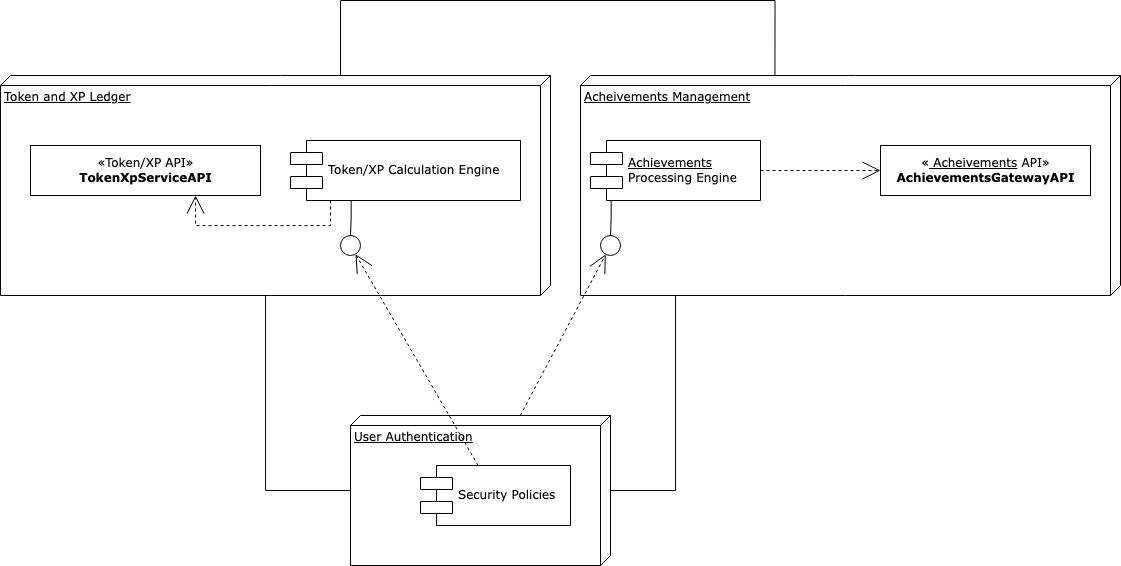
\includegraphics[width=1\textwidth]{src/assets/chapters/reward-deployement-diagram.drawio.png}
    \caption{ Reward System Architecture Overview}
    \label{fig:reward_system_architecture_overview}
\end{figure}

\section{Design}
This phase of the project builds upon our foundational work to refine and expand the architecture of our reward system. We delve into key considerations, decisions, and enhancements introduced in this release, focusing particularly on how our models support the reward functionalities.

\subsection{Static Modeling}
The static modeling phase has been pivotal in defining the core structure of our reward system. We have continued to refine our data models and database schema to align with our evolving functional requirements and business rules.

\subsubsection{Domain Model}
We have structured our reward system around three primary classes: RewardLog, UserRewards, and Achievement. These classes are designed to seamlessly interact within our system to facilitate efficient reward management and user engagement through achievements.



\subsection{Classes Description}
\begin{table}[H]
    \renewcommand{\arraystretch}{1.5} % Padding
    \centering
    \medskip
    \begin{tabularx}{1\textwidth} {
            | >{\hsize=0.4\hsize\linewidth=\hsize\raggedright\arraybackslash}X
            | >{\hsize=1.6\hsize\linewidth=\hsize\raggedright\arraybackslash}X |}
        \hline
        \rowcolor{primary} \textbf{Class Name} & \textbf{Description} \\
        \hline
        RewardLog & Models individual reward transactions, capturing details like user ID, reward type (XP, token), and the source of the reward (e.g., completing a task or manual adjustment). \\
        \hline
        UserRewards & Models the cumulative rewards and achievements for a user, providing a comprehensive overview of their progress and tokens. \\
        \hline
        Achievement & Details the achievements that users can earn, including the criteria for earning them and the rewards associated with them. \\
        \hline
        Rank & Represents the various ranks users can achieve. Each rank includes a label (e.g., 'Ground Floor'), the levels required to reach the rank, and a description that highlights the significance of the rank. This class helps track user progression and assigns appropriate ranks based on their XP levels. \\
        \hline
    \end{tabularx}
\end{table}



For these classes, we have defined the following associations:
\begin{itemize}
    \item Each UserRewards document embeds an array of Achievement subdocuments, reflecting the user's progress towards various achievements.
    \item RewardLog entries are linked to specific actions or events, such as achievement completions, which can update the UserRewards document.
\end{itemize}
 we illustrate the extension of our class diagram, highlighting newly added classes and associations for clarity.

\subsubsection{Data Dictionary}
In table IV.4, we provide a comprehensive overview of the key data elements used in our model, detailing how they interact and are structured within our database. This dictionary will cover the essential attributes for each class, such as userId, type, and source in RewardLog, and how they are indexed for performance and uniqueness.

\subsubsection{Logical Data Model}
Building on the foundation laid by the first version of our logical data model, our MVP, we now present an updated model that retains the original structure while introducing necessary expansions for this release. This updated model provides insights into the relationships and structure of our data entities, reflecting the full scope of the initial solution. Figure IV.2 illustrates the class diagram, showing how new and existing entities are interconnected within our system.


 \begin{figure}[H]
    \centering
    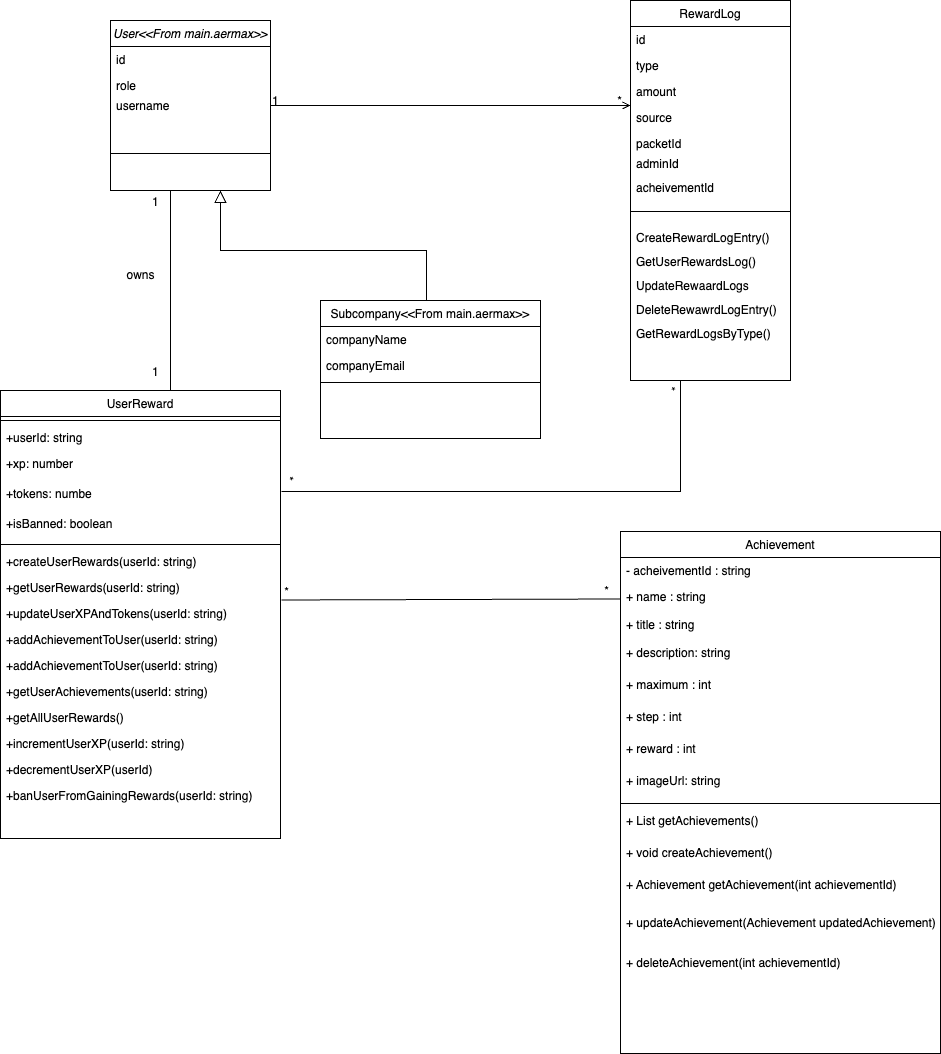
\includegraphics[width=0.9\textwidth]{src/assets/chapters/reward--system-classDiagram.drawio.png}
    \caption{ Data Model Architecture}
    \label{fig:reward_system_architecture_overview}
\end{figure}
\subsection{Data Dictionary}
\subsection{Data Dictionary for RewardLog}

\subsection{Data Dictionary for RewardLog}
\begin{table}[H]
    \renewcommand{\arraystretch}{1.5} % Padding
    \centering
    \caption{Data Dictionary for RewardLog}
    \medskip
    \begin{tabularx}{\textwidth} {
            | >{\hsize=0.8\hsize\linewidth=\hsize\raggedright\arraybackslash}X
            | >{\hsize=1.7\hsize\linewidth=\hsize\raggedright\arraybackslash}X
            | >{\hsize=0.6\hsize\linewidth=\hsize\raggedright\arraybackslash}X
            | >{\hsize=0.9\hsize\linewidth=\hsize\raggedright\arraybackslash}X |}
        \hline
        \rowcolor{primary} \textbf{Field} & \textbf{Description} & \textbf{Type} & \textbf{Constraints} \\
        \hline
        userId & User's unique identifier & string & Required \\
        \hline
        type & Type of reward (e.g., xp, token) & enum & Required \\
        \hline
        amount & Amount of reward given & number & Required \\
        \hline
        source & Source of reward (e.g., close\_packet, manual\_adjustment, achievement) & enum & Required \\
        \hline
        packetId & Identifier for the reward packet, if applicable & string & Optional \\
        \hline
        adminId & Administrator's identifier managing the reward & string & Optional \\
        \hline
        achievementId & Reference to associated achievement & ObjectId & Optional \\
        \hline
    \end{tabularx}
\end{table}

\subsection{Data Dictionary for UserRewards}
\begin{table}[H]
    \renewcommand{\arraystretch}{1.5} % Padding
    \centering
    \caption{Data Dictionary for UserRewards}
    \medskip
    \begin{tabularx}{\textwidth} {
            | >{\hsize=0.8\hsize\linewidth=\hsize\raggedright\arraybackslash}X
            | >{\hsize=1.5\hsize\linewidth=\hsize\raggedright\arraybackslash}X
            | >{\hsize=0.6\hsize\linewidth=\hsize\raggedright\arraybackslash}X
            | >{\hsize=1.1\hsize\linewidth=\hsize\raggedright\arraybackslash}X |}
        \hline
        \rowcolor{primary} \textbf{Field} & \textbf{Description} & \textbf{Type} & \textbf{Constraints} \\
        \hline
        userId & User's unique identifier & string & Required \\
        \hline
        xp & Total experience points & number & Default: 0 \\
        \hline
        tokens & Total tokens & number & Default: 0 \\
        \hline
        reason & Reason for reward adjustment & string & Optional \\
        \hline
        achievements & Array of achievements (subdocument) & subdocument & Optional \\
        \hline
        isBanned & Whether the user is banned from receiving rewards & boolean & Default: false \\
        \hline
    \end{tabularx}
\end{table}

\subsection{Data Dictionary for Achievement}
\begin{table}[H]
    \renewcommand{\arraystretch}{1.5} % Padding
    \centering
    \caption{Data Dictionary for Achievement}
    \medskip
    \begin{tabularx}{\textwidth} {
            | >{\hsize=0.8\hsize\linewidth=\hsize\raggedright\arraybackslash}X
            | >{\hsize=1.5\hsize\linewidth=\hsize\raggedright\arraybackslash}X
            | >{\hsize=0.6\hsize\linewidth=\hsize\raggedright\arraybackslash}X
            | >{\hsize=1.1\hsize\linewidth=\hsize\raggedright\arraybackslash}X |}
        \hline
        \rowcolor{primary} \textbf{Field} & \textbf{Description} & \textbf{Type} & \textbf{Constraints} \\
        \hline
        name & Name of the achievement & string & Required, Unique \\
        \hline
        reward & Reward amount for achieving this milestone & number & Default: 0 \\
        \hline
        step & Incremental steps required to achieve the milestone & number & Default: 1 \\
        \hline
        maximum & Maximum progress needed to complete the achievement & number & Default: 1 \\
        \hline
        title & Title of the achievement & string & Required \\
        \hline
        description & Description of the achievement & string & Required \\
        \hline
        imageUrl & URL of the image associated with the achievement & string & Required \\
        \hline
        createdBy & Identifier of the user who created the achievement & string & Required \\
        \hline
        updatedBy & Identifier of the user who last updated the achievement & string & Required \\
        \hline
    \end{tabularx}
\end{table}
\section{Dynamic Modeling}
In this section, we explore the dynamic aspects of our reward system, focusing on the interactions and communication behaviors between components and actors within our system. 

\subsection{User Interaction Workflow}
This flowchart illustrates the dynamic interactions users have with our system, depicting the process flow and decision points encountered during typical user sessions. Understanding these interactions helps us optimize the user experience and streamline how rewards and achievements are managed in response to user actions.

 \begin{figure}[H]
    \centering
    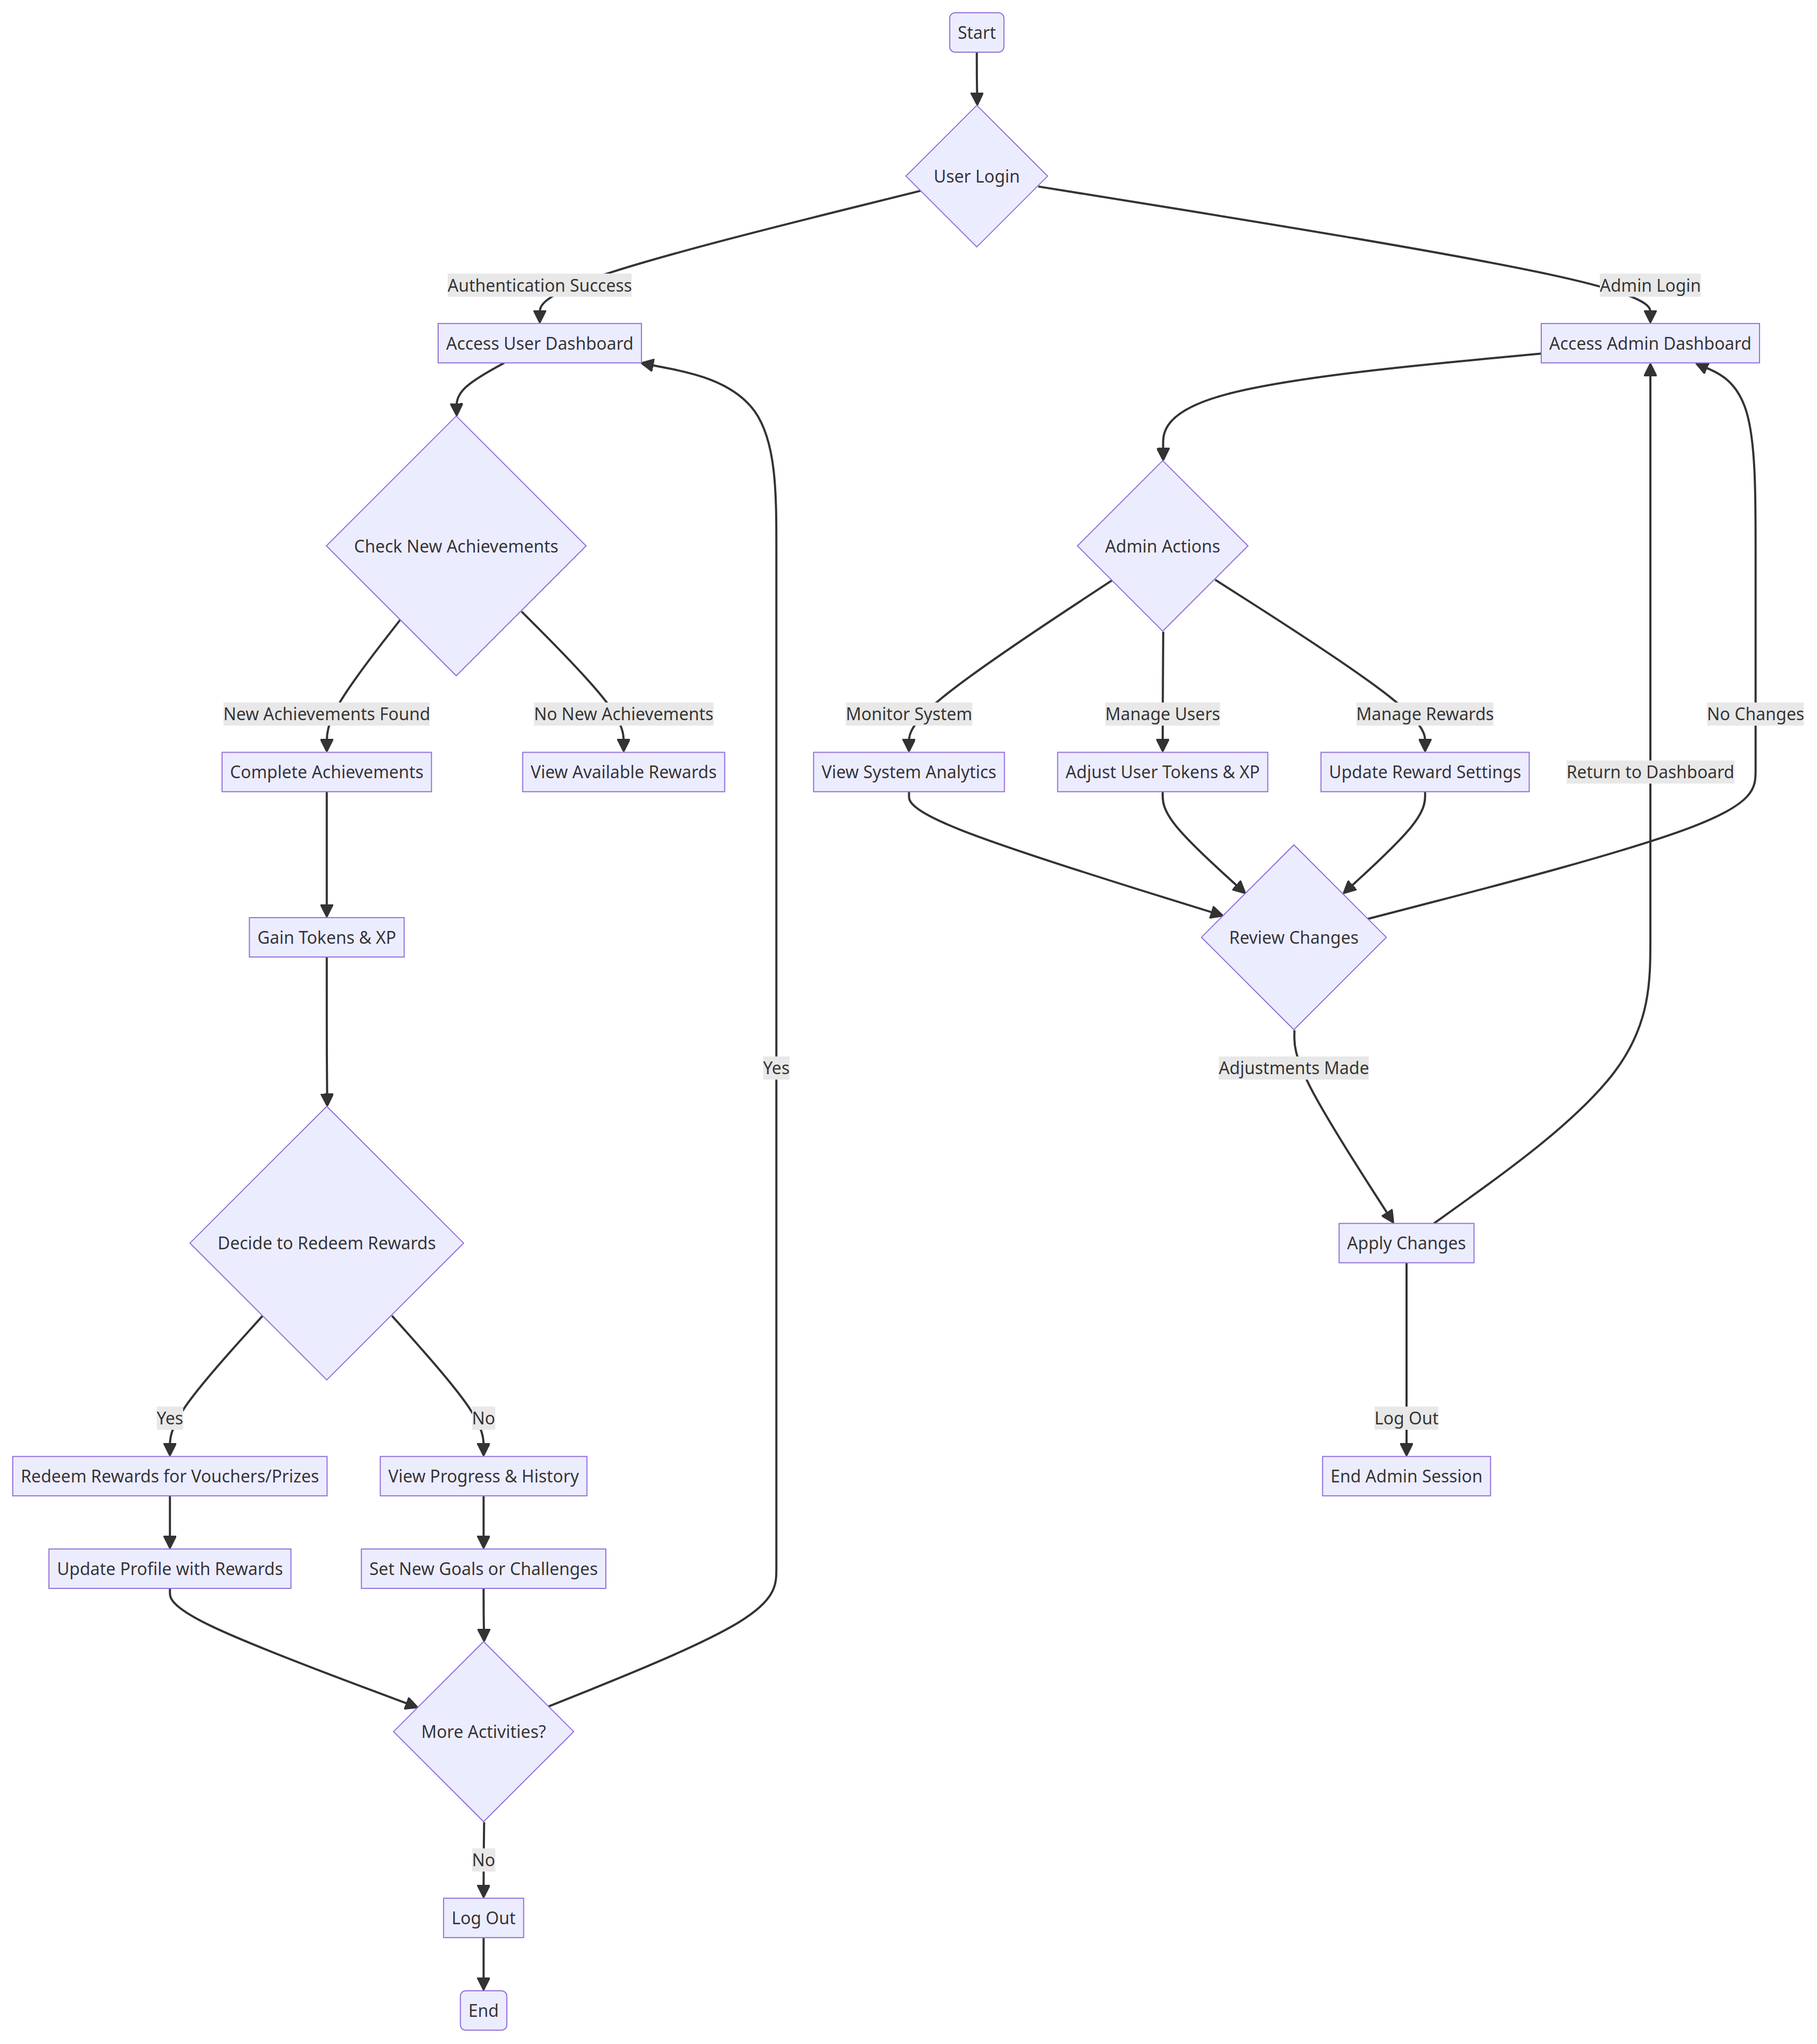
\includegraphics[width=0.9\textwidth]{src/assets/chapters/Reward-System_Activity-Flow.png}
    \caption{ Data Model Architecture}
    \label{fig:reward_system_architecture_overview}
\end{figure}

\subsection{Admin Sequence Diagram}
The admin sequence diagram concisely outlines the steps an admin takes to manage the reward system, from login through various tasks like adjusting tokens and XP. It clarifies the admin's interactions within the system and assists in streamlining administrative functions for optimal efficiency.


% Here you would include your admin sequence diagram figure
\begin{figure}[H]
    \centering
    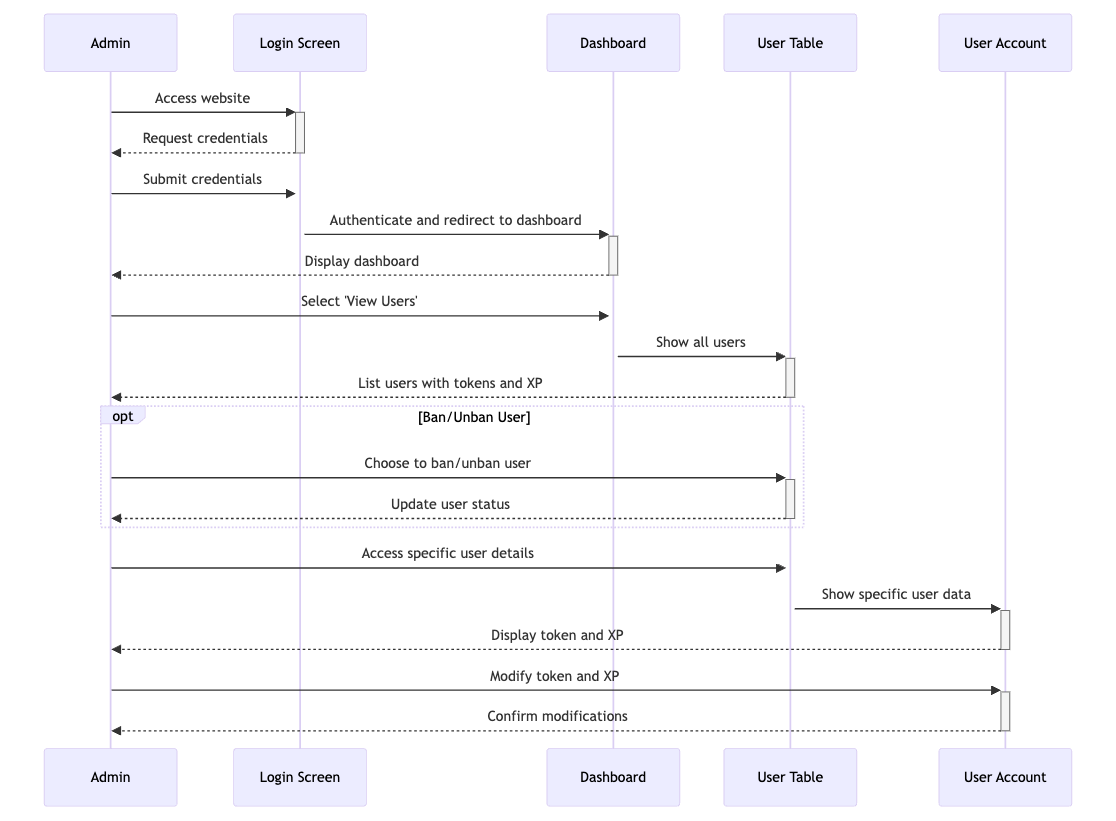
\includegraphics[width=0.9\textwidth]{src/assets/chapters/AdminSequencediagram.png}
    \caption{Admin Sequence Diagram for the Reward System}
    \label{fig:admin_sequence_diagram}
\end{figure}
\subsection{Subcompany User Sequence Diagram}
This sequence diagram depicts the key steps a subcompany user takes within the reward system, from login to earning rewards. It streamlines the user journey, highlighting how users interact with the system and the resulting workflow, thereby ensuring an experience that is both user-friendly and aligned with the system's goals.


% Include the figure for the subcompany user sequence diagram here
\begin{figure}[H]
    \centering
    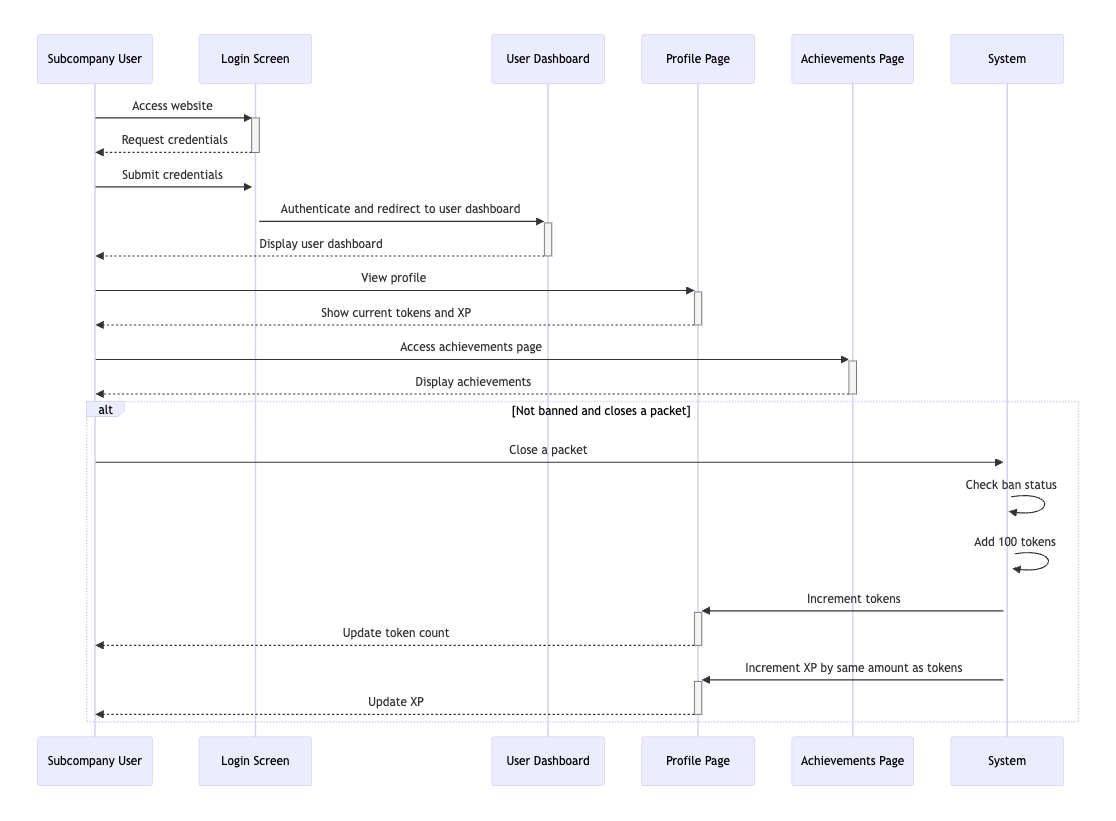
\includegraphics[width=0.9\textwidth]{src/assets/chapters/subbcomapny_user_sequence_diagram.png}
    \caption{Sequence Diagram for Subcompany User Interactions in the Reward System}
    \label{fig:subcompany_user_sequence_diagram}
\end{figure}

\section{Software Architecture}
Following the design phase, we chose to implement a separate microservice built with NestJS to enhance the scalability and maintainability of our reward system. This microservice architecture allows for isolated development and deployment, which simplifies updates and scaling operations.

\subsection{Microservice Architecture}
The new microservice integrates seamlessly with existing services such as the operation-service and user-service. It communicates via RabbitMQ, a robust message broker that ensures reliable and efficient message handling between services. This approach not only improves the system's responsiveness but also its overall resilience, allowing each component to operate independently yet cohesively.

\paragraph{Benefits of NestJS and RabbitMQ:}
\begin{itemize}
    \item \textbf{NestJS:} Provides a scalable framework for building efficient and fail-safe systems, thanks to its use of modern JavaScript features and its integration with TypeScript.
    \item \textbf{RabbitMQ:} Facilitates secure and flexible cross-service communication, enhances fault tolerance, and manages load effectively, even under high demand.
\end{itemize}

This architectural decision supports our goal of creating a dynamic, reliable, and scalable reward system, prepared to handle increasing loads and complexity as the Aermax platform grows.

\begin{figure}[H]
    \centering
    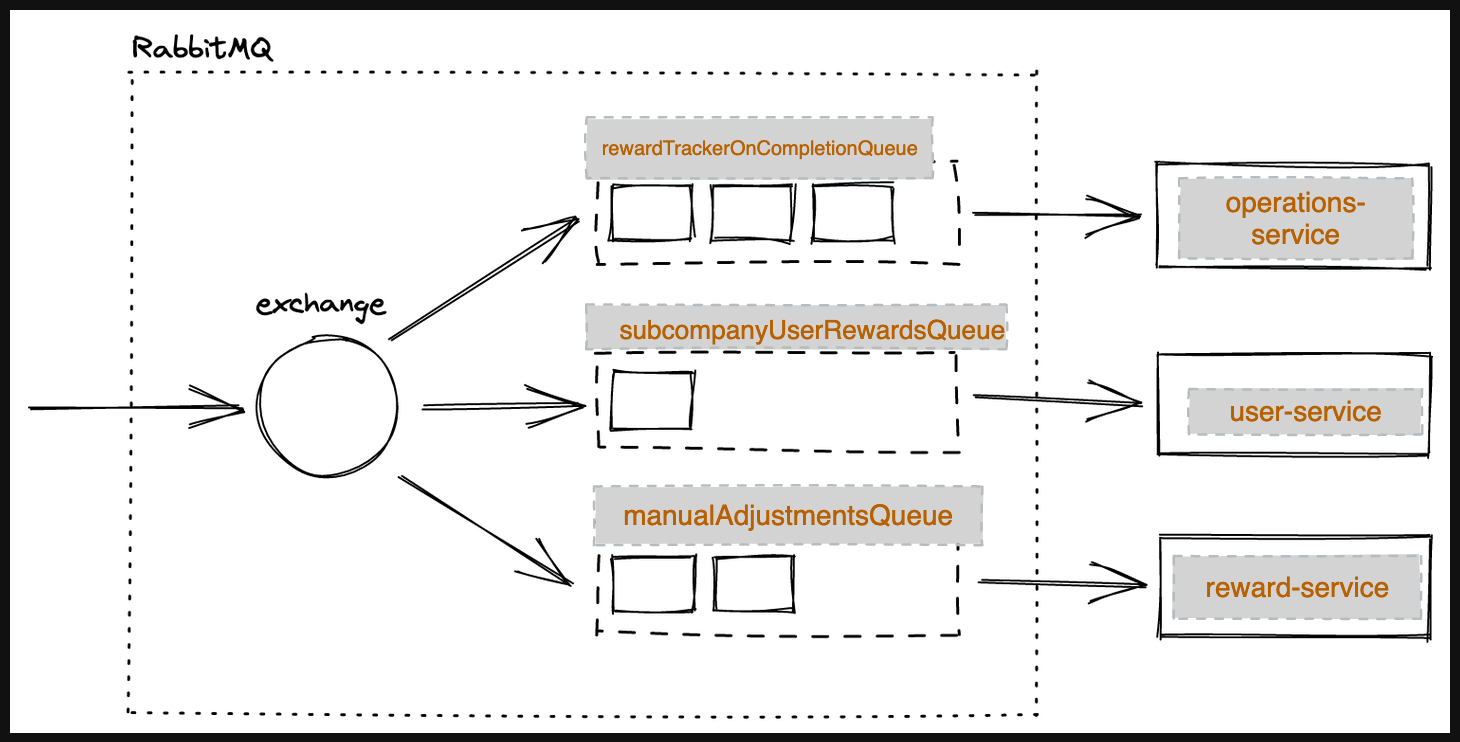
\includegraphics[width=0.9\textwidth]{src/assets/chapters/rmq.png}
    \caption{Microservice Communication Example via RabbitMQ in the Reward System}
    \label{fig:microservice_communication_rabbitmq}
\end{figure}

\section{Technology Stack and Framework Selection}

\subsection*{Why We Chose RabbitMQ}
The decision to choose RabbitMQ as our message broker was based on specific needs for our system's communication and architecture:

\begin{itemize}
    \item \textbf{Decoupling of Services:} RabbitMQ provides independence between services, facilitating a more maintainable and flexible architecture.
    \item \textbf{Asynchronous Communication:} It enables services to communicate without synchronous waits, increasing efficiency.
    \item \textbf{Scalability:} RabbitMQ supports even message distribution, which is essential for scaling services effectively.
    \item \textbf{Reliability and Fault Tolerance:} It ensures message delivery reliability, even when some services are down.
    \item \textbf{Centralized Management:} RabbitMQ offers centralized management of message flows, improving monitoring and control.
    \item \textbf{Ordering and Prioritization:} It manages the order and priority of message handling, which is crucial for process sequencing.
\end{itemize}

\paragraph*{Comparison of Message Brokers}
Below is a comparison of message brokers supported by NestJS, highlighting their main features and common use cases:
\begin{table}[H]
    \centering
    \caption{Comparison of Message Brokers}
    \label{tab:message_brokers_comparison}
    \renewcommand{\arraystretch}{1.5} % Padding
    \begin{tabularx}{\textwidth} {
            | >{\hsize=0.7\hsize\linewidth=\hsize\raggedright\arraybackslash}X
            | >{\hsize=1.2\hsize\linewidth=\hsize\raggedright\arraybackslash}X
            | >{\hsize=1.1\hsize\linewidth=\hsize\raggedright\arraybackslash}X |}
        \hline
        \rowcolor{primary} \textbf{Message Broker} & \textbf{Main Features} & \textbf{Use Case} \\
        \hline
        Kafka & High throughput, scalability, fault tolerance, and durable storage & Event streaming, log aggregation \\
        \hline
        MQTT & Lightweight, low bandwidth requirement, designed for IoT devices & IoT, real-time messaging \\
        \hline
        RabbitMQ & Flexible routing, reliable messaging, multiple protocol support & Complex routing, service decoupling \\
        \hline
        Redis & In-memory data structure, high performance, supports pub/sub & Caching, real-time analytics \\
        \hline
        NATS & At-most-once delivery, lightweight, supports queuing & Microservices communication, IoT \\
        \hline
        gRPC & High-performance RPC, supports bi-directional streaming & Inter-service communication, APIs \\
        \hline
    \end{tabularx}
    \end{table}

Our selection of RabbitMQ aligns with our system's need for a robust, reliable, and flexible communication backbone.

\section{Message Broker Operation}

\subsection*{How Does a Message Broker Work?}
A message broker like RabbitMQ plays a critical role in modern software architectures by managing communications between different parts of a system. It acts as a middleman that allows services to send and receive messages without knowing the complexities of each other’s design, location, or technology.

\paragraph*{Example: PDF Creation Process}
Consider a PDF creation process in a web application, which is a typical use case for a message broker. Here’s how it operates:

\begin{enumerate}
    \item A user initiates a PDF creation request from the website application interface.
    \item The application, acting as the \textbf{Producer}, publishes a message to the RabbitMQ \textbf{Exchange}. This message contains the user’s information and the request details.
    \item RabbitMQ routes the message to the appropriate \textbf{Queue} based on the message's content and the queue's binding rules.
    \item The \textbf{Consumer}, which could be a PDF Creator Worker, listens to the queue, consumes the message, and processes the PDF creation.
\end{enumerate}

This process showcases how RabbitMQ facilitates asynchronous communication, ensuring the application’s responsiveness and reliability. The Producer is decoupled from the Consumer, allowing for independent scaling and maintenance.

\begin{figure}[H]
    \centering
    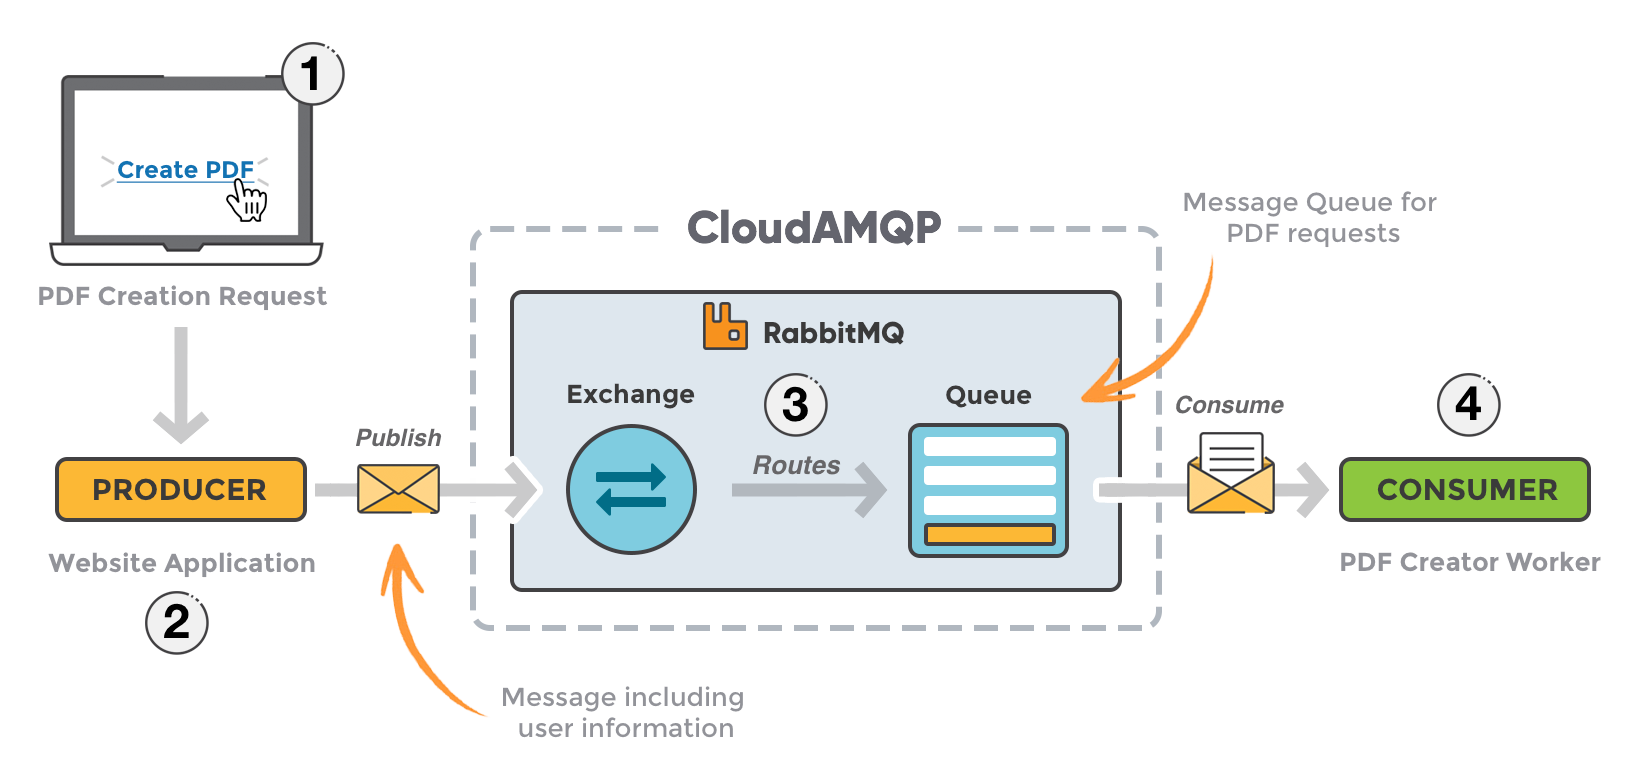
\includegraphics[width=0.9\textwidth]{src/assets/chapters/rabbitmqexample.png} % Replace with your image path
    \caption{Example of Message Broker Workflow in PDF Creation}
    \label{fig:message_broker_workflow}
\end{figure}

The diagram (Figure \ref{fig:message_broker_workflow}) visualizes this workflow, clarifying the roles of Producers, Exchanges, Queues, and Consumers within the RabbitMQ ecosystem.

\section{NestJS as the Development Framework}

NestJS was selected for its:

\begin{itemize}
    \item Strong support for TypeScript, enhancing code reliability.
    \item Modular architecture, which simplifies scalability and maintenance.
    \item Built-in support for microservices and integration with RabbitMQ.
    \item Dependency injection system, promoting code modularity and reusability.
    \item Growing community and rich ecosystem, providing extensive resources.
    \item Similarity to Angular, offering an easier learning curve for developers.
\end{itemize}

These attributes of NestJS align well with our system’s goals for robust and maintainable microservice development.


\thispagestyle{plain} % Remove header
\addcontentsline{toc}{chapter}{General Conclusion}
\section*{General Conclusion}


% Generate a webography, for more styles
% see - https://www.overleaf.com/learn/latex/Bibtex_bibliography_styles#Table_of_stylename_values
\renewcommand\bibname{Webography}
\bibliographystyle{unsrt}
\bibliography{references}
\addcontentsline{toc}{chapter}{Webography}
\clearpage


% Very big diagrams, pictures or schemas go here
% List of appendices
\begin{appendices}
    \begin{figure}[H]
        \centering
        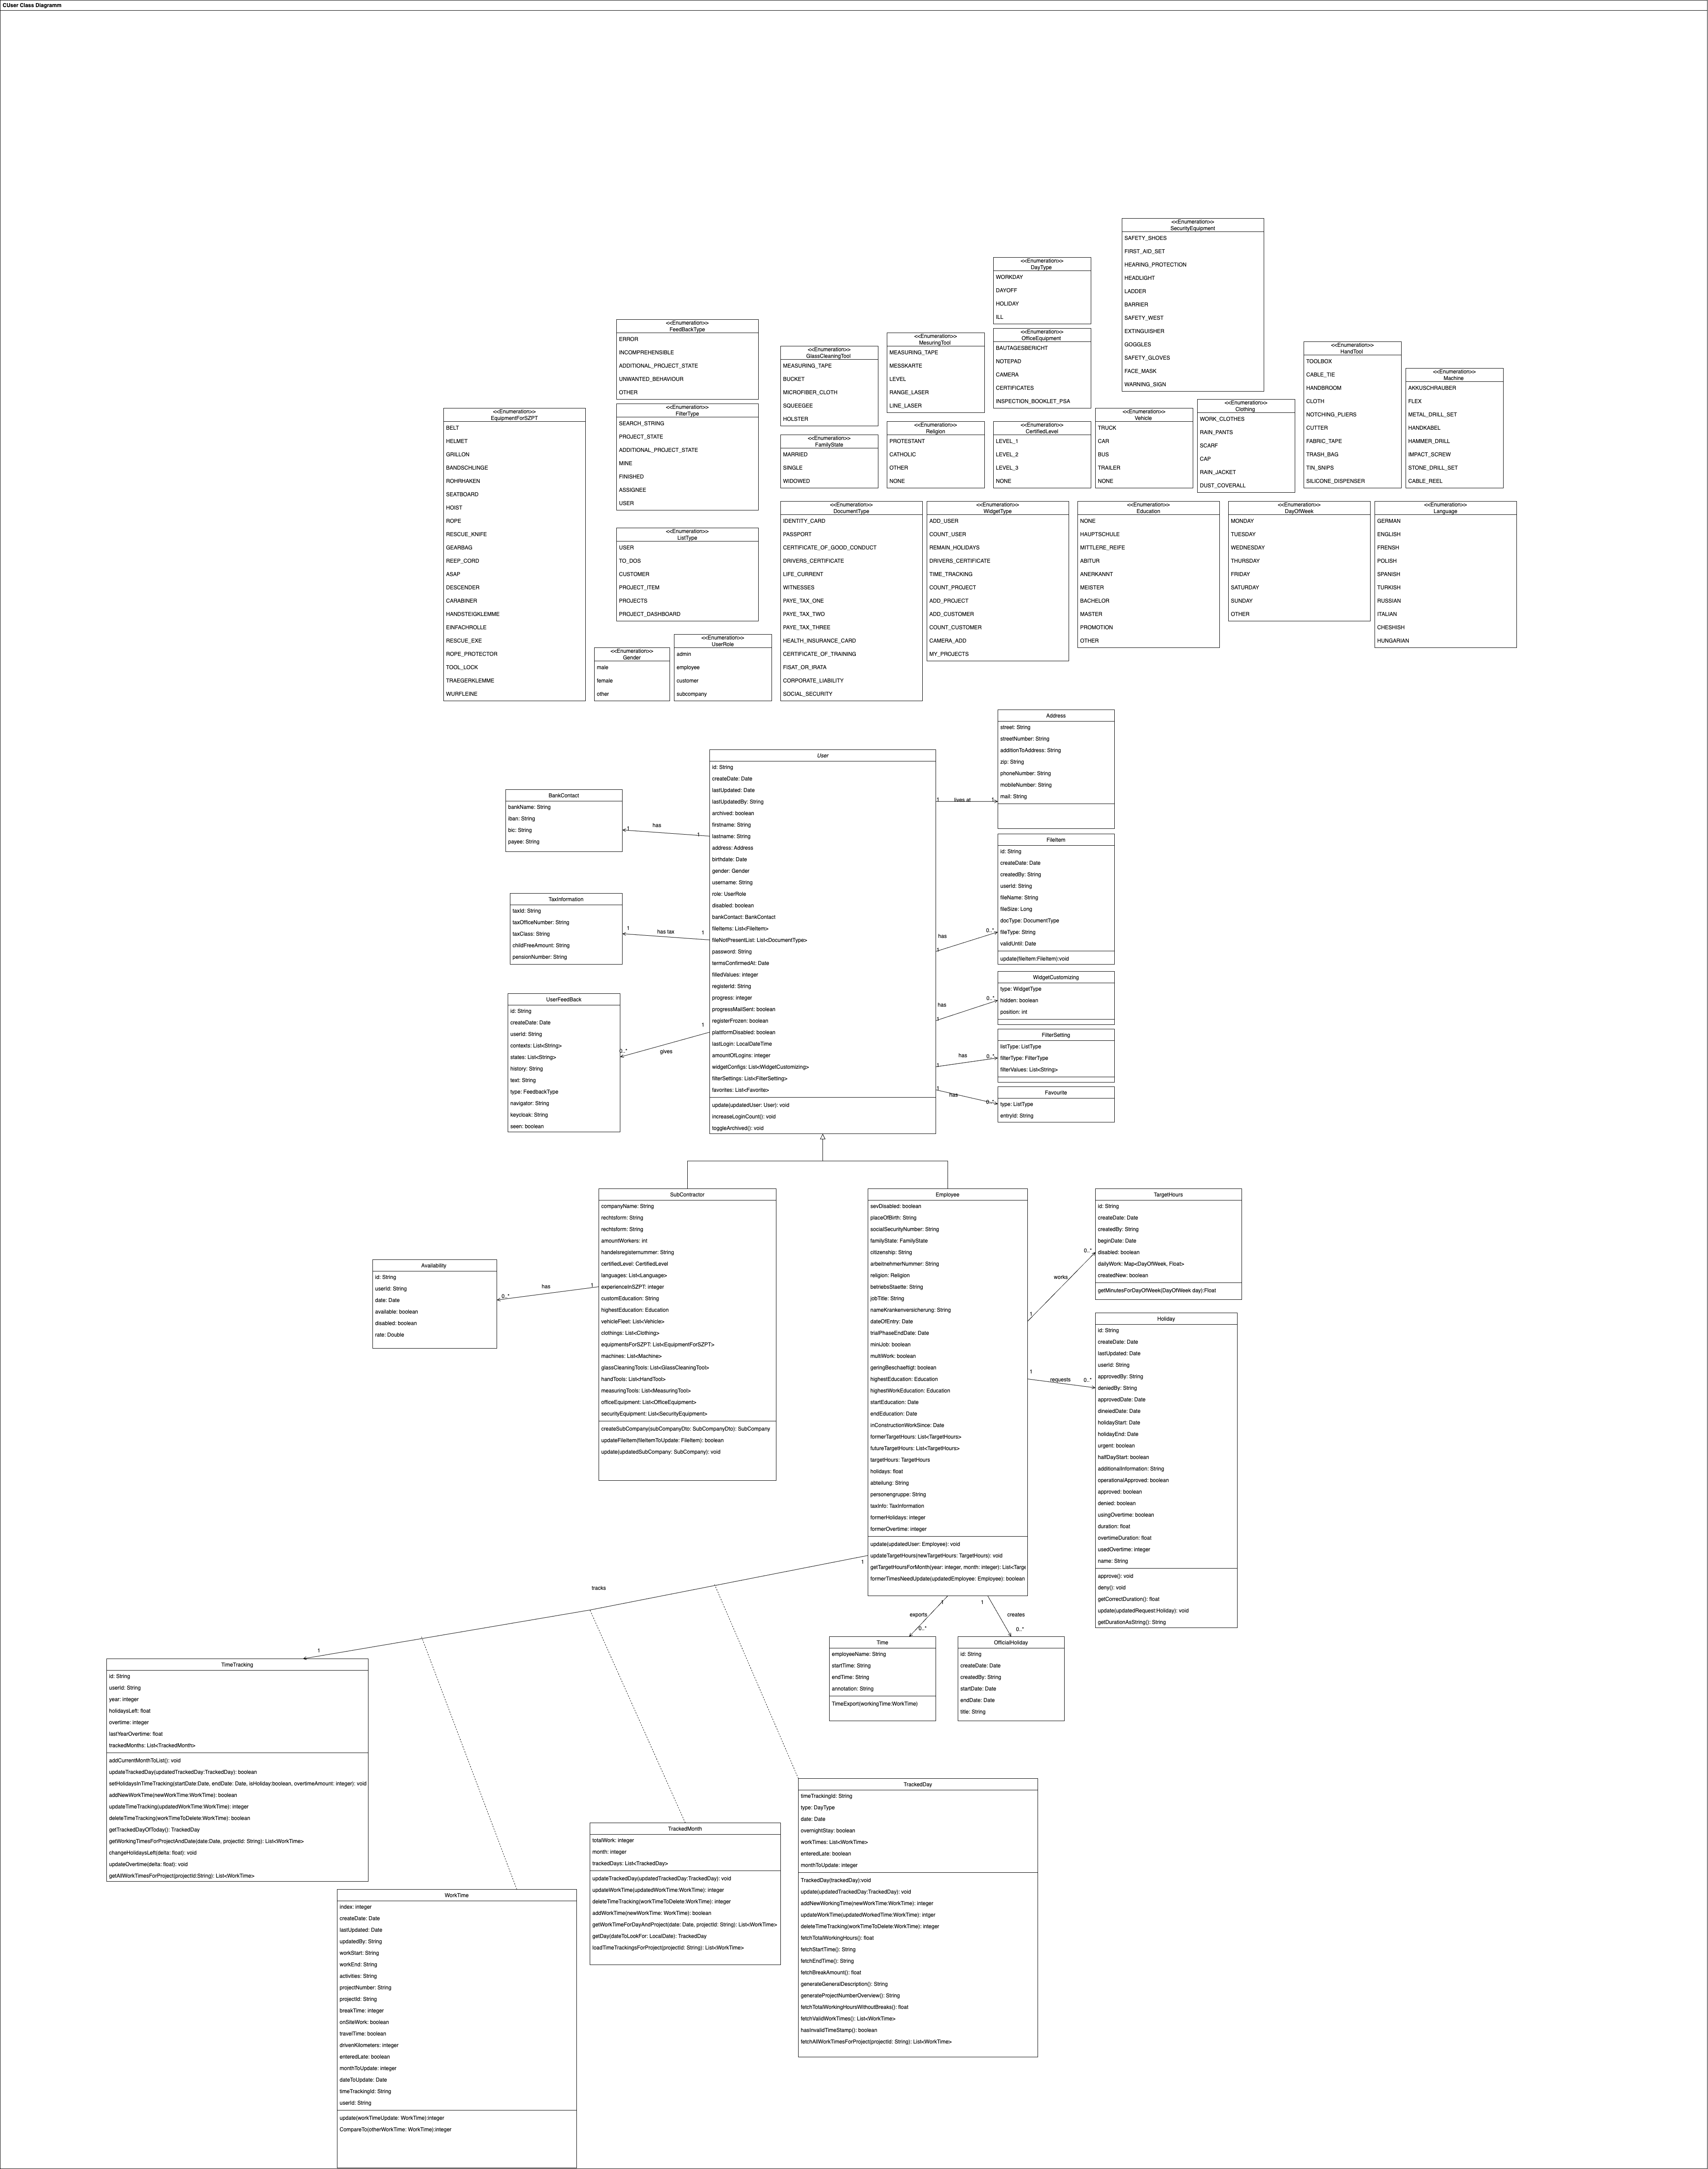
\includegraphics[width=\linewidth,height=\textheight]{src/assets/diagrams/Class_Diagram_related_to_user.png}
        \captionof{figure}{Class Diagram Related to User in main.aermax}
        \label{fig:class-diagram-related-to-user}
    \end{figure}    
\end{appendices}

\end{document}